\documentclass{book}

\usepackage{graphicx}
\usepackage{moreverb}
\usepackage{amsmath}
\usepackage{alltt}
\usepackage{rotating}
\usepackage{subfigure}
\usepackage{toc}
\usepackage{xspace}
\usepackage{makeidx}

\newcommand{\extref}[1]{$\S$\ref*{#1}}   % No hyperlink. For external refs. \extref
\newcommand{\comma}{\> ,}
\newcommand{\period}{\> .}
\newcommand{\wt}{\widetilde}
\newcommand{\grv}{\textasciigrave}
\newcommand{\hyperbf}[1]{\textbf{\hyperpage{#1}}}
\newcommand{\Ss}{\(^*\)}
\newcommand{\Dd}{\(^\dagger\)}

\newcommand{\AND}{&& \hskip -17pt\relax}
\newcommand{\CR}{\\}
\newcommand{\CRNO}{\nonumber \\}
\newcommand{\dstyle}{\displaystyle}

\newcommand{\Begineq}{\begin{equation}}
\newcommand{\Endeq}{\end{equation}}
\newcommand{\NoPrint}[1]{}

\newcommand{\pow}[1]{\cdot 10^{#1}}
\newcommand{\Bf}[1]{{\bf #1}}
\newcommand{\bfr}{\Bf r}

\newcommand{\bmad}{{\sl Bmad}\xspace}
\newcommand{\tao}{{\sl Tao}\xspace}
\newcommand{\mad}{{\sl MAD}\xspace}
\newcommand{\cesr}{{\sl CESR}\xspace}

\newcommand{\sref}[1]{\S\ref{#1}}
\newcommand{\Sref}[1]{Sec.~\sref{#1}}
\newcommand{\cref}[1]{Chapter~\ref{#1}}

\newcommand{\Newline}{\hfil \\ \relax}

\newcommand{\eq}[1]{{(\protect\ref{#1})}}
\newcommand{\Eq}[1]{{Eq.~(\protect\ref{#1})}}
\newcommand{\Eqs}[1]{{Eqs.~(\protect\ref{#1})}}

\newcommand{\vn}{\ttcmd}           % For variable names
\newcommand{\vni}{\ttcmdindx}
\newcommand{\cs}{\ttcmd}           % For code source
\newcommand{\cmd}{\ttcmd}          % For Unix commands
\newcommand{\rn}{\ttcmd}           % For Routine names
\newcommand{\tn}{\ttcmd}           % For Type (structure) names
\newcommand{\bn}[1]{{\bf #1}}       
\newcommand{\toffset}{\vskip 0.01in}
\newcommand{\rot}[1]{\begin{rotate}{-45}#1\end{rotate}}

\newcommand{\data}{{\mbox{data}}}
\newcommand{\reference}{{\mbox{ref}}}
\newcommand{\model}{{\mbox{model}}}
\newcommand{\base}{{\mbox{base}}}
\newcommand{\design}{{\mbox{design}}}
\newcommand{\meas}{{\mbox{meas}}}
\newcommand{\var}{{\mbox{var}}}

\newcommand\ttcmd{\begingroup\catcode`\_=11 \catcode`\%=11 \dottcmd}
\newcommand\dottcmd[1]{\texttt{#1}\endgroup}

\newcommand\ttcmdindx{\begingroup\catcode`\_=11 \catcode`\%=11 \dottcmdindx}
\newcommand\dottcmdindx[1]{\texttt{#1}\endgroup\index{#1}}

\newcommand{\St}{$^{st}$\xspace}
\newcommand{\Nd}{$^{nd}$\xspace}
\newcommand{\Th}{$^{th}$\xspace}
\newcommand{\B}{$\backslash$}
\newcommand{\W}{$^\wedge$}

\newcommand{\cbar}[1]{\overline C_{#1}}

\newlength{\dPar}
\setlength{\dPar}{1.5ex}

\newenvironment{example}
  {\vspace{-3.0ex} \begin{alltt}}
  {\end{alltt} \vspace{-2.5ex}}

\newcommand\Strut{\rule[-2ex]{0mm}{6ex}}

\newenvironment{Itemize}
  {\begin{list}{$\bullet$}
    {\addtolength{\topsep}{-1.5ex} 
     \addtolength{\itemsep}{-1ex}
    }
  }
  {\end{list} \vspace*{1ex}}

\newcommand{\Section}[1]{\section{#1}\indent\vspace{-3ex}}

\newcommand{\SECTION}[1]{\section*{#1}\indent\vspace{-3ex}}

% From pg 64 of The LaTex Companion.

\newenvironment{ventry}[1]
  {\begin{list}{}
    {\renewcommand{\makelabel}[1]{\textsf{##1}\hfil}
     \settowidth{\labelwidth}{\textsf{#1}}
     \addtolength{\itemsep}{-1.5ex}
     \addtolength{\topsep}{-1.0ex} 
     \setlength{\leftmargin}{5em}
    }
  }
  {\end{list}}


\setlength{\textwidth}{6.25in}
\setlength{\oddsidemargin}{0.25in}
\setlength{\evensidemargin}{0.00in}
\setlength{\textheight}{8.5in}
\setlength{\topmargin}{0in}

\makeindex

\begin{document}

\thispagestyle{empty}

\begin{flushright}
\large
  Revision: 0.3.2 \\
  April 30, 2006 \\
\end{flushright}

\vfill

{
\begin{center}
{\Huge \sf\bf The} \\
\vskip 0.1in
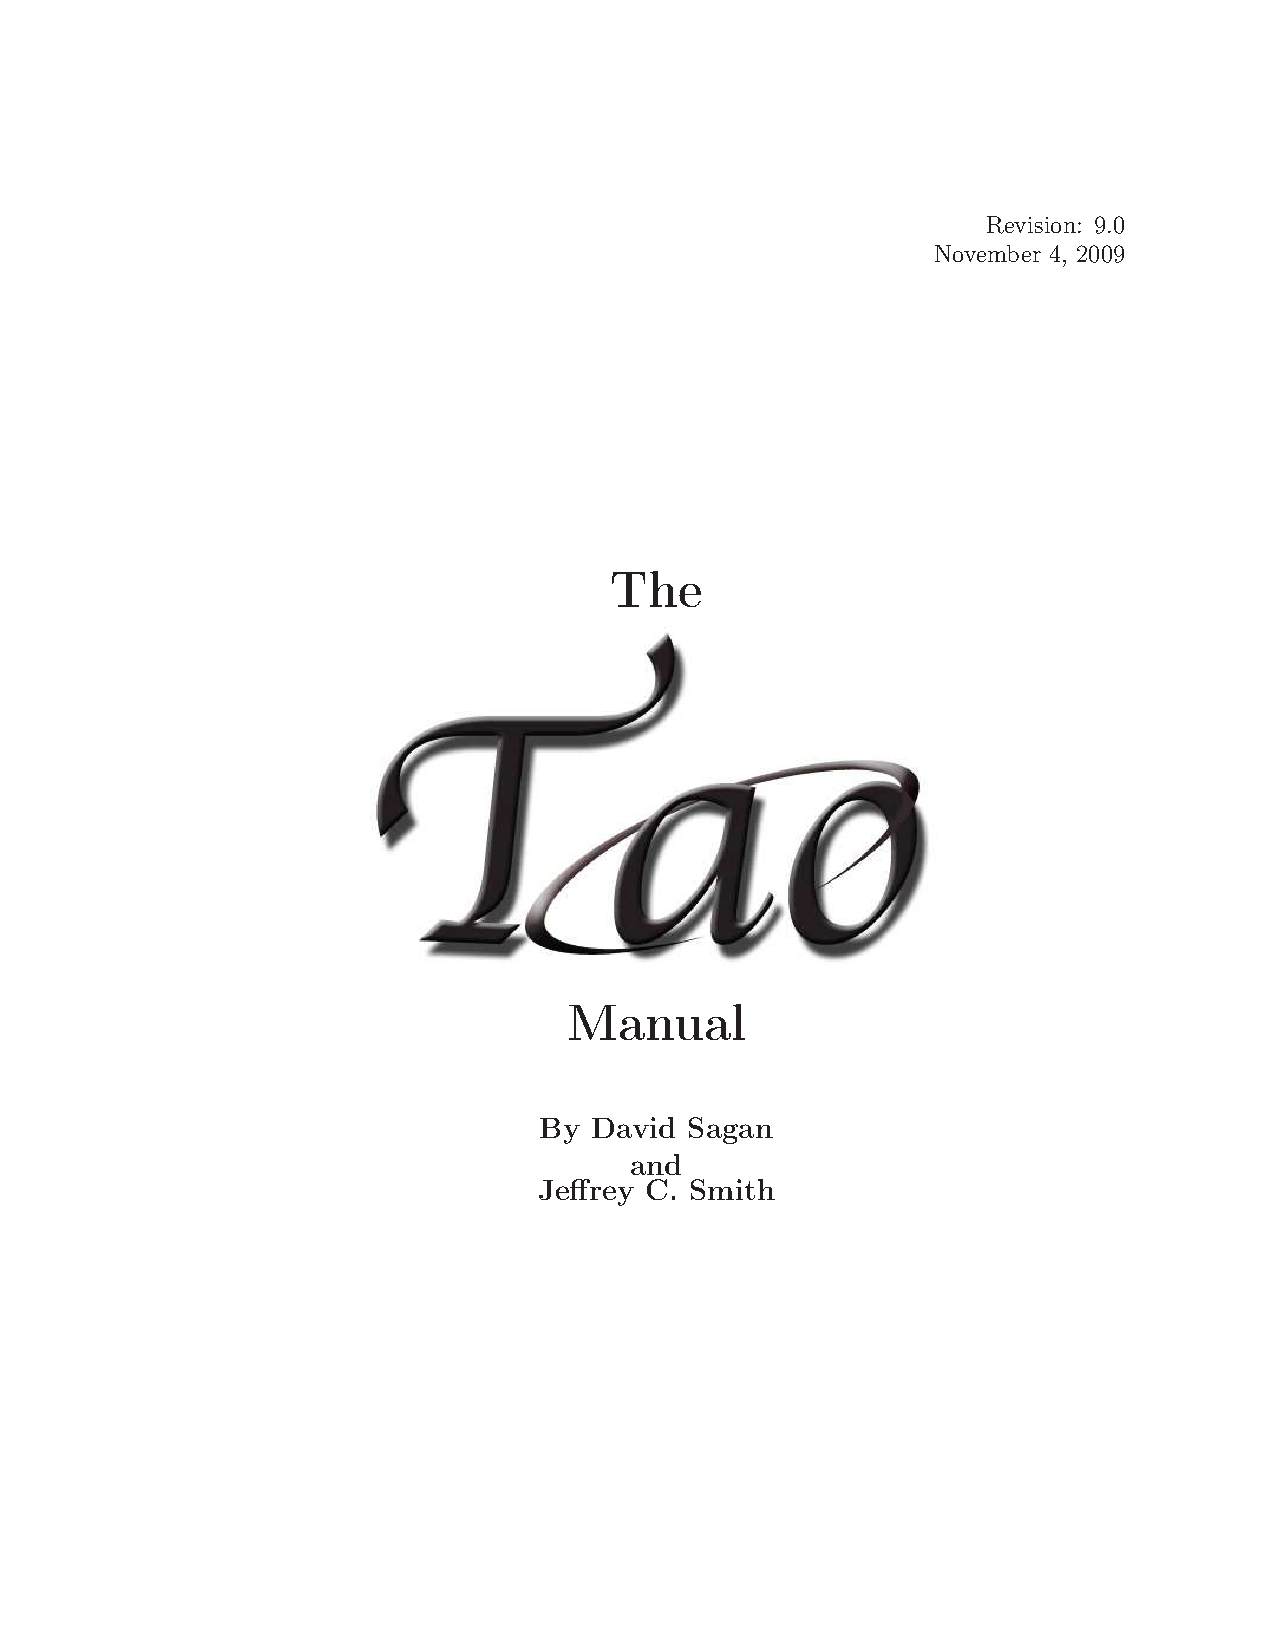
\includegraphics[width=10cm]{tao.psfig} \\
\vskip 0.1in
{\Huge \sf\bf Manual} \\
\vskip 0.4in
{\Large \sf\bf By David Sagan \\ and \\ Jeffrey C. Smith} \\
\end{center}
}

\vskip 1in
\begin{center}
{\Huge \bf *** DRAFT ***}
\end{center}
\vfill
\break


%----------------------------------------------------------------
{
\setlength{\parskip}{\dPar}
\setlength{\parindent}{0ex}

\section*{Introduction}

The strength of \bmad is that, as a subroutine library, it provides a
flexible framework from which sophisticated simulation programs may
easily be developed.  The weakness of \bmad comes from its strength:
\bmad cannot be used straight out of the box. Someone must put the
pieces together into a program. This means that \bmad is
complementary to a general purpose program like
\MAD\cite{b:maduser,b:madphysics}: If \mad can solve the problem at
hand you don't need \bmad. If there are no programs that do what you
want, or they are too slow, then \bmad is very useful.

As a consequence of \bmad being a software library this manual serves
two masters: The programmer who wants to develop applications and
needs to know about the inner workings of \bmad, and the user who
simply needs to know about the \bmad standard input format and about
the physics behind the various calculations that \bmad performs.

To this end, this manual is divided into three parts. The first two
parts are for both the user and programmer while the third part is
meant just for programmers. Part~I gives the conventions used by
\bmad --- coordinate systems, magnetic field expansions, etc. ---
along with some of the physics behind the calculations. By necessity,
the physics documentation is brief and the reader is assumed to be familiar
with high energy accelerator physics formalism. Part~II discusses the
\bmad lattice input standard.  The \bmad lattice input standard was
developed using the \mad lattice input standard as a starting
point. \mad (Methodical Accelerator Design) is a widely used
stand--alone program developed at CERN by Christoph Iselin for
charged--particle optics calculations. Since it can be convenient
to do simulations with both \mad and \bmad, differences and
similarities between the two input formats are noted. 
Finally, Part~III gives the nitty--gritty details of the \bmad
subroutines and the structures upon which they are based.

More information, including the most up--to--date version of this
manual, can be found at the \bmad web site at
\begin{example}
  http://www.lepp.cornell.edu/~dcs/bmad
\end{example}
\index{Bmad!information}

Errors and omissions are a fact of life for any reference work and
comments from you, dear reader, are therefore most welcome. Please
send any missives (or chocolates, or any other kind of sustenance) to:
\begin{example}
  David Sagan <dcs16@cornell.edu>
\end{example}
\index{Bmad!error reporting}

It is my pleasure to express appreciation to people who have
contributed to this effort: To David Rubin for his support, to Etienne
Forest for use of his remarkable PTC/FPP library not to mention his
patience in explaining everything to me, to Mark Palmer for all his
work porting \bmad to different platforms, to Hans Grote for granting
the adaptation of figures in the \mad manual for use in this one, to
Richard Helms, Kim Moore, Jeremy Urban, Jeff Smith, and Mike Forster
for their help, and last but not least to my wife Flora who put up
with me at 1am in the morning when I was working on \bmad.


}

%----------------------------------------------------------------
\tableofcontents
\listoffigures
%% \listoftables

%----------------------------------------------------------------
\setlength{\parskip}{\dPar}
\setlength{\parindent}{0ex}

\part{Concepts and Tutorial}

\chapter{Tao Concepts}
\label{c:concepts}

\tao stands for ``Tool for Accelerator Optics''. \tao is a general
purpose program for simulating high energy particle beams in
accelerators and storage rings. This tutorial assumes you are already
familiar with the basics of particle beam dynamics and its
formalism. There are several books that introduce the topics very
well. A good place to start is \textit{The Physics of Particle
Accelerators} by Klaus Wille.

\tao is based on the \bmad\cite{b:bmad} subroutine library. An
understanding of the nitty-gritty details of the routines that
comprise \bmad is not necessary, however, one should be familiar with
the conventions that \bmad uses and this is covered in the \bmad
manual.

So, what is \tao good for? A large variety of applications. It's
versatility is that it's easily expandable. Think of it as an
accelerator design and analysis environment. But even without any
customizations, \tao will do much analysis. 

This chapter discusses how \tao is organized. After you are familiar
with the basics of \tao, there is a hands-on tutorial in
Chapter~\sref{c:tutorial}. After you get more familiar with \tao, you
might be interested exploit its versatility by extending \tao to do
custom calculations. For this, see Chapter~\ref{c:custom-tao}.

%----------------------------------------------------------------
\section{The Orginization of Tao: The Super\_Universe}
\label{s:orginization}

Many simulation problems fall into one of three categories: 
\begin{itemize}
\item 
Design a lattice subject to various constraints.
\item
Simulate errors and changes in machine parameters. For example, you want to
simulate what happens to the orbit, beta function, etc., when you change
something in the machine. 
\item 
Simulate machine commissioning including simulating data measurement and
correction. For example, you want to know what steering strength changes will
make an orbit flat.
\end{itemize}
Programs that are written to solve these types of problems have common
elements: You have variables you want to vary in your model of your
machine, you have "data" that you want to view, and, in the first two
categories above, you want to match the machine model to the data (in
designing a lattice the constraints correspond to the data).

With this in mind, \tao was structured to implement the essential
ingredients needed to solve these simulation problems.  
The information that \tao knows about can be divided into five
categories:
\begin{description}
  \item[Lattice] \Newline   
Machine layout and component strengths, and the beam orbit (\sref{s:lattice}).
  \item[Data] \Newline
Anything that can be measured.
For example: The orbit of a particle or the lattice beta 
functions, etc. (\sref{c:data})
  \item[Variables] \Newline
Essentially, any lattice parameter or initial condition that can be varied.
For example: quadrupole strengths, etc. (\sref{s:variable-overview}).
  \item[Plotting]  \Newline
Information used to draw graphs, display the lattice 
floor plan, etc. (\sref{s:plotting}).
  \item[Global] \Newline
Global parameters.
\end{description}

\index{Super_universe}
\index{Structure}
The information in \tao deals is organized in a hierarchy of
\vn{``structures''}. At the top level, everything known to \tao is
placed in a structure called the \vn{super_universe}.

Within the \vn{super_universe} lies one or more \vn{universes}
(\sref{s:universe}), each \vn{universe} containing a particular
machine lattice and its associated data. This allows for the user to
do analysis on multiple machines or multiple configurations of a
single machine at the same time. The \vn{super_universe} also contains
\vn{variable}, \vn{plotting}, and \vn{global} information.

%------------------------------------------------------------------------
\section{The Universe}
\label{s:universe}
\index{Universe}

The \tao \vn{super_universe} (\sref{s:orginization}) contains one or
more \vn{universes}.  A \vn{universe} contains a \vn{lattice}
(\sref{s:lattice}) plus whatever data (\sref{c:data}) one wishes to
study within this lattice (i.e. twiss parameters, orbit, phase,
etc.). Actually, there are three lattices within each universe: the
\textbf{design} lattice, \textbf{model} lattice and \textbf{base}
lattice. Initially, when \tao is started, all three lattices are
idential and correspond to the lattice read in from the lattice
description file (\sref{s:init-lat}).

There are several situations in which multipole universes are
useful. One case is where there are multiple machines. For example, a
transfer line connected to a storage ring. In this case, one universe
will correspond to the transfer line and another universe will
correspond to the storage ring. 

Another case where multiple universes are useful is where data has
been taken under different machine conditions. For example, Suppose
that the beam orbit in a machine has been taken with a given steering
element set at some value and then the orbit is again measured but
this time with some other element set to some value. To determine what
quadrupole settings will best reprodue the data, two universes can be
setup. One universe associated with one set of data and the second
universe associated with the other set of data. Variables can be
defined to simultaneously vary the corresponding quadrupoles in each
universe and \tao's built in optimizer can vary the variables until
the data as determined from the \vn{model} lattice (\sref{s:lattice})
matches the measured data.

%------------------------------------------------------------------------
\section{Lattices}
\index{Lattice}
\label{s:lattice}

A \vn{lattice} consists of a machine description (the strength and
placement of elements such as quadrupoles and bends) along with the
beam orbit through them. There are actually three types of lattices:
  \vspace*{-3ex}
  \begin{description}
  \item[Design Lattice] \Newline 
The \vn{design} lattice corresponds to the lattice read in from the
lattice description file (\sref{s:init-lat}). In many instances this
is the particular lattice that one wants the actual physical machine
to conform to. The \vn{design} lattice is fixed. Nothing is alowed to
vary in this lattice.
  \item[Model Lattice] \Newline
Except for some commands that explicitly set the \vn{base} lattice,
all \tao commands to vary lattice variables vary quantities in the
\vn{model} lattice. In particular, things like orbit correction
involve varying \vn{model} variables until the \vn{data} as calculated
from the \vn{model} match the \vn{data} as actually measured.
  \item[Base Lattice] \Newline
It is sometimes convenient to designate a reference lattice so that
changes in the \vn{model} from the reference point can be examined.
This reference lattice is called the \vn{base} lattice. The \vn{set}
command (\sref{s:set}) is used to transfer information from the
\vn{design} or \vn{model} lattices to the base lattice.
  \end{description}

%------------------------------------------------------------------------
\section{Variables}
\label{s:variable-overview}
\index{Variables}


A variable is anything that can be varied. For example, quadrupole
strengths or the initial position of a particle in a LINAC. Any
variable can be varied using the \vn{change} command
(\sref{s:change}). However it can be convenient to set up within \tao
predefined groups of variables. For example, the optimizer
(\sref{s:optimizer}) will only work with such blocks.


Variables control attributes of elements in the model lattice of one
or more universes. They are not the same thing as attributes in
lattice elements.  Instead, they \textit{control} attributes in
lattice elements. They are more akin to \bmad \textit{overlays}. A
given variable may control a single attribute of one element in one or
more universes. If you want a variable to control a collection of
elements like a \bmad \textit{group} then you need to insert the
appropriate group in your lattice. Variables are what you vary in
order to change your model lattice. You can also change your model
lattice by directly changing and lattice element attribute. However,
if you plan on doing any optimization then you will need to use
variables.

\index{v1_var}


Blocks of variables are associated with what is called a \vn{v1_var}
structure and each of these structures has a \vn{name} with which to
refer to them in \tao commands. For example, if \vn{quad_k1} is the
name of a \vn{v1_var} then \vn{quad_k1[5]} referres to the variable 
with index 5. 

A given variable may control a single attribute of one element in a
\vn{model} lattice of a single universe or it can be configured to
simultaneously control an element attribute across multiple
universes. Any one variable cannot control more than one attribute of
one element. However, a variable may control an overlay or group
element, which in turn controls numerous elements.

Each individual variable has a number of values associated with it:
  \vspace*{-3ex}
  \index{Variable!measured}\index{Variable!reference}
  \index{Variable!model}\index{Variable!design}\index{Variable!base}
  \begin{description}
  \item[Measured Value] \Newline
The Value as obtained at the time of the \vn{data} measurement.
  \item[Reference Value] \Newline
The Value as obtained at the time of the \vn{reference} data  measurement.
  \item[Model Value] \Newline
The value as given in the \vn{model} lattice.
  \item[Design Value] \Newline
The value as given in the \vn{design} lattice.
  \item[Base Value] \Newline
The value as given in the \vn{base} lattice.
  \end{description}
These components and others can be refered to using the notaion \vn{|name} where
\vn{name} is the appropriate name for the component. The list of
components that can be set or refered to are:
\begin{example}
  quad_k1[1]|meas      ! Value at time of data measurement
  quad_k1[1]|ref       ! VAlue at time of the reference data measurement
  quad_k1[1]|model     ! Value in the model lattice
  quad_k1[1]|base      ! Value in the base lattice
  quad_k1[1]|design    ! Value in  the design lattice
  quad_k1[1]|weight    ! Weight used in the merit function.
  quad_k1[1]|old       ! Scratch value.
  quad_k1[1]|step      ! For fitting/optimization: What is considered a small change.
  quad_k1[1]|exists    ! Logical
  quad_k1[1]|good_var  ! Logical
  quad_k1[1]|good_ref  ! Logical
  quad_k1[1]|good_user ! Logical
  quad_k1[1]|good_opt  ! Logical
  quad_k1[1]|good_plot ! Logical
\end{example}

Use the \vn{show var} (\sref{s:show}) command to view variable information

%------------------------------------------------------------------------
\section{Plotting}\index{Plotting}
\label{s:plotting}

\begin{figure}
  \centering
  \includegraphics{plot.eps}
  \caption[A plot has a collection of graphs.]
{A plot has a collection of graphs and a graph has a 
collection of curves. A plot becomes visible when it is associated
with some region on the page using the \vn{place} command. Note that
on the actual page the plot/region border is not visible.}
  \label{f:plot}
\end{figure}

Some definitions:
  \vspace*{-3ex}
\begin{description}
\item[Curve] \Newline
A \vn{curve} is a set of (x,y) points to be plotted.
\item[Graph] \Newline
A \vn{graph} consists of horizontal and vertical axes along with a set
of \vn{curve}s that are plotted within the graph. 
\item[Plot] \Newline
A \vn{plot} is essentially a collection of \vn{graphs}.
\item[Page] \Newline
The \vn{page} refers to the x--window where graphics are displayed or the 
corresponding printed graphics page.
\item[Region] \Newline
The \vn{page} is divided up into a number of rectangles called
\vn{regions}. \vn{Regions} may overlap.
\end{description}

The plot initialization file (cf.~Chapter~\ref{c:init}) defines a set
of \vn{template plots}. A \vn{template} defines what type of data is
to be plotted (orbit, coupling, etc.), how many \vn{graphs} there are,
what the scales are for the \vn{graph} axes, how the \vn{graph}s are
laid out, etc.  The plot initialization file also defines a set of
\vn{region}s within the \vn{page}. Any \vn{template plot} can be
placed in any region. Using the \vn{place} command (see
Chapter~\ref{c:command} for a full descriptions of all commands) one
can assign a particular \vn{template plot} to a particular region for
plotting.  The relationship between \vn{region}, \vn{plot},
\vn{graph}, and \vn{curve} is shown graphically in
Figure~\ref{f:plot}.

Figures~\ref{f:plot-page1} and \ref{f:plot-page2} show examples of a
plot \vn{page}. Figure~\ref{f:plot-page1} was generated by defining
two regions called \vn{top} and \vn{bottom} in the plot initialization
file. The \vn{top} region was defined to cover the upper half of the
\vn{page} and the \vn{bottom} region was defined to cover the bottom
half. \vn{Template plots} were defined to plot phase and orbit data
from a defined set of detector elements in the lattice. Each
\vn{template plot} defined two graphs which in both cases where
assigned the names \vn{x} and \vn{y}. The orbit \vn{template plot} was
placed in the \vn{top} region and the phase \vn{template plot} was
placed in the \vn{bottom} region. The horizontal axis numbering is by
detector \vn{index}.  Displayed plots are referred to by the
\vn{region} name (\vn{top} and \vn{bottom} in this case). Individual
graphs and curves are referred to using the nomenclature
\vn{region.graph.curve}. Thus, in this example, the horizontal orbit graph
would be referred to as \vn{top.x}.  Using the \vn{plot} command one
can then specify \vn{who} is plotted. \vn{who} refers to
\vn{measured}, \vn{reference}, \vn{model}, \vn{base}, and/or
\vn{design} data.  Notice that the same \vn{template plot} can be
assigned to different \vn{regions} and the plots in different
\vn{regions} can have different scales for their axes or different
\vn{who}. In the example in Figure~\ref{f:plot-page1}, \vn{who} for
the \vn{top} plot is \vn{model} and for the \vn{bottom} plot it is
\vn{model - design}.

Plots may be referred to by their template name or by the name of the 
region they are placed in. For example, the orbit plot in 
Figure~\ref{f:plot-page1} may be referred to using the region name (\vn{top})
or the template name (\vn{orbit}). A template may be placed in multiple regions.
For example, you may wish to plot the \vn{model} data for the orbit in one
region and the  \vn{design} data for the orbit in another region. In this case 
the command \vn{scale orbit} would scale the plots in both regions while to scale
the plot in only one of the regions you would need to use the region name. A graph
of a plot is specified using the format \vn{plot_name.graph_name} where \vn{plot_name}
is a template or region name and \vn{graph_name} is the name of the graph. For example,
if the horizontal orbit graph of the ]\vn{orbit} plot is named \vn{x} then it would
be referred to as \vn{orbit.x} or \vn{top.x}. A curve
within a graph is specified using the format \vn{plot_name.graph_name.curve_name}.

The \vn{use}, \vn{veto}, \vn{restore}, and \vn{clip} commands are used
to control what data is used in fitting the model to the data in the
optimization process (see Chapter~\ref{c:opti}). The general rule is
that these commands only effect measured and reference data. If
plotting \vn{model}, \vn{design} and/or \vn{base} data then the data
will always been displayed. If plotting \vn{meas} and/or \vn{ref} data
then the data displayed will vary with these commands.  \vn{meas} or
\vn{ref} data vetoed for display is also vetoed for fitting.  However,
measured data that is off the vetical or horizontal scale may still be
used by the optimizer unless vetoed with the \vn{veto} or \vn{clip}
command.  If there are data points off the vertical scale then
``**Limited**'' will appear in the upper right-hand corner of the
graph. If plotting measured data then these points off scale will
still be used by the optimizer.

The \vn{x-axis} and \vn{x-scale} commands are used to set the axis
type and scale for each graph. The axis type can be either \vn{index},
\vn{ele_index} or \vn{s} which corresponds to the data index number,
element index number and longitudinal poisition in the lattice (from
element 0) respectively.

Figure~\ref{f:plot-page2} shows another example of a plot \vn{page}.
In this case the \vn{page} was generated by again defining two
vertically stacked regions but in this case the regions have different
heights.  A \vn{template plot} with a single graph was placed in the
bottom most \vn{region}.  This \vn{graph} contains a \vn{key_table}.
A \vn{key_table} is used in conjunction with \vn{single mode} and is
explained in Chapter~\ref{c:single}. A \vn{template plot} containing
five \vn{graphs} was placed in the uppermost region. The uppermost
\vn{graph} of this \vn{template plot} contains a \vn{lat_layout} which
shows the placement of lattice elements.  What elements are displayed
in a \vn{lat_layout} and what shapes they are represented by is
specified in the initialization file. The horizontal scale is
longitudinal position (\vn{s}).  The remaining four graphs show
disperion and beta data from two different universes representing the
low energy and high energy transport in an energy recovery linac. The
individual data points here (hard to see in this example) have been
slaved to the \vn{lat_layout} and represent the beta and dispersion at
the edges of the displayed elements in the \vn{lat_layout}.


\begin{figure}
  \centering
  \includegraphics[width=5in]{plot-page1.eps}
  \caption{Example of a plot page}
  \label{f:plot-page1}
\end{figure}

\begin{figure}
  \centering
  \includegraphics[width=5in]{plot-page2.eps}
  \caption{Another example of a plot page.}
  \label{f:plot-page2}
\end{figure}

\vfill
\break
%------------------------------------------------------------------------
\section{Single Character Input}
\index{Single Mode}

Sometimes it is convenient to be able to vary variables using single
key strokes without having to type a carriage return.  With \tao, this
is possible using what is called \vn{single mode}. This is distinct
from \vn{line mode} where commands to \tao are typed at the command
line with a carriage return signaling the end of the command. 

The \vn{single mode} initialization file associates variables with
certain keyboard keys so that when these keys are pressed the value of
the variable is varied. This association between variables and keys is
called a \vn{key table}. See Chapter~\sref{c:single} for more details.

%------------------------------------------------------------------------
\section{Tracking Types}
\index{Tracking!Types}

\index{track_type}
\index{tao_global_struct}
The are three types of tracking implemented in \tao: single particle
tracking, many particle multi-bunch tracking and macroparticle
multi-bunch tracking. Single particle tracking is just that, the
tracking of a single particle through the lattice. Many particle
multi-bunch tracking creates a gaussian distribution of particles at
the beginning of the lattice and tracks each particle through the
lattice, including any wakefields. Macroparticle tracking takes a beam
distribution and tracks the centroids and sigmas of the
``macro-particles'' through the lattice, including any wakefields.
Single particle tracking is used by default. The
\vn{global%track_type} parameter (\sref{s:globals}), which is set in
the initialization file, is used to set the tracking.


Particle spin tracking has also been set up for single particle and many
particle tracking. See Sections~\sref{s:globals} and \sref{s:beam-init} for
details on setting up spin tracking.

\vn{Note:} Macroparticle tracking has not been used for some time and
the underlying code used for macroparticle tracking is dormant. The
use of macroparticle tracking is thus discouraged. If you have a need
for this please contact David Sagan.

%------------------------------------------------------------------------
\section{Lattice Calculation}\index{Lattice!calculation of}
\label{s:lat-calc}

After each \tao command is processed the lattice and ``merit''
function is recalculated then the plot window is regenerated. The
merit function determines how well the \vn{model} fits the measured
data. See Chapter~\ref{c:opti} for more information on the merit
function and its use by the optimizer.

Below are the steps taken after each \tao command execution:
\begin{enumerate}
  \item 
The data and variables used by the optimizer is re-determined. This is
affected by commands such as \vn{use, veto,} and \vn{restore} and any
changes in the status of elements in the ring (e.g. if any elements
have been turned off).
  \item 
If changes have been made to the lattice (e.g. variables changed) then
the model lattice for all universes will be recalculated. The
\vn{model} orbit, linear transfer matrices and twiss parameters are
recalculated for every element. All data types will also be calculated
at each element specified in the initialiation file.  For single
particle tracking the linear transfer matrices and twiss parameters
are found about the tracked orbit. For particle bunch and
macroparticle bunch tracking the linear transfer matrices and twiss
parameters are calculated from the beam distribution.  Tracking is
performed using the tracking method defined for each element
(i.e. Bmad Standard, Symplectic Lie, etc...). See the \bmad Reference
manual for details on tracking and finding the linear transfer
matrices and twiss parameters.
  \item 
The \vn{model} data is recalculated from the \vn{model} orbit, linear
transfer matrices, twiss parameters, particle beam information and
global lattice parameters.  Any custom data type calculations are
performed \textit{before} the standard \tao data types are calculated.
  \item 
Any user specified data post-processing is performed in
\vn{tao_hook_post_process_data}.
  \item 
The contributions to the merit function from the variables and data are
computed.
  \item 
Data and variable values are transfered to the plotting structures.
  \item 
The plotting window is regenerated.
\end{enumerate}




\chapter{``Vanilla'' Tao}
\label{c:vanilla_tao}

%----------------------------------------------------------------
\section{Before we start...}
\label{s:before_beginning}

\tao is readily customizable. All the bookkeeping is taken care of
automatically and all you need to do custom analysis is write the
subroutines pertinent to your project. However beginners are advised
to start with ``out of the box'' \tao while getting to know the
program. This tutorial starts here and will then show you how to
customize \tao for your specific purposes.

\subsection{Getting and Compiling Tao}
\index{Compiling Tao}
\label{s:get_and_compile}

The following instructions are for Cornell people. If you are not at
Cornell then the source files can be obtained at:
\begin{example}
  http://www.lepp.cornell.edu/bmad
\end{example}

In any case help may be obtained by contacting David Sagan
\cmd{<dcs16@cornell.edu>} or Jeff Smith \cmd{<js344@cornell.edu>}.

Before running \tao at Cornell the appropriate environmental variables
must be set. The way \tao is developed is that the source code is kept
in a central ``repository'' which is controlled by a software package
called \vn{CVS}. Every so often (typically about once a week) a copy
of the source code in the repository is made and a version of \tao is
compiled from this copy. This is called a ``release''. There are two
major releases: One called ``devel'' is made from the very latest
code. There is also a ``current'' release which comes from older
code. The general idea is that devel should have the latest stuff but
current should be more stable (have less bugs). In practice, since
\tao is new and the bugs are still being worked out, the devel release
is typically less buggy and hence is devel is what is recommended. To
set the environmental variables to point to the devel release do the
following.  If you are using the bash shell put the following in your
\vn{.login} file:
\begin{example}
  CESRLIB=devel
  . /home/cesrulib/bin/cesrdefs
\end{example}
If you are using tcsh put in your \vn{.login} file: 
\begin{example} 
  setenv CESRLIB devel
  source /home/cesrulib/bin/cesrdef
\end{example}
This sets the appropriate environmental variables to point to the
``devel'' ``release

After setting up the environmental variables \tao is run with the command
\begin{example}
  \$CESR_EXE/tao
\end{example}
If there has been a bug fix that you need which is in the CVS
repository but not yet in the devel release, you need to create and
use a local copy of \tao. To checkout a copy of \tao from the CVS
repository use the command \cmd{'cesrcvs co tao'} in the directory
from where you want to run \tao, (hereto referred to as
\vn{ROOT}). The checked out copy of \tao will be put in a directory
\cs{ROOT/tao}. Basically the only time a local copy of \tao is needed
is when there have been changes made to CVS that are needed that
haven't found their way to the released version. Once you have created
a local copy of \tao you may need to update it from time to time when
changes to the repository have been made by the maintainers of
\tao. To do this use the command \cmd{'cesrcvs update'} in the
\cs{ROOT/tao} directory. Note: Unless you are a maintainer, you do not
have privileges to modify the repository.



If you already have a
local copy of \tao and want to update

From the newly created \cs{ROOT/tao} directory type `\cmd{gmake}' to
create the libraries and then type `\cmd{gmake -f M.tao}' to create
the ``vanilla'' \tao program. Vanilla \tao is the basic \tao program
without any user customizations. If you are using a custom version of
\tao then follow the compiling directions from the custom \tao
author. Keep in mind that command syntax and usage may vary between
custom versions of \tao (this is a \textit{feature}, \textbf{not} a
bug!).

Once \tao has compiled go to the subdirectory \cs{ROOT/tao/program}
and type \cmd{../../bin/tao} to run ``vanilla'' \tao. This directory
contains all the configuration files to get everything working. The
first time you run the program it will need to create a digested \bmad
lattice file for the included lattice. This may take a few minutes.

\subsection{Customizing Tao}
\index{customizing Tao}

After you are familiar with the basics of \tao you are ready to fully
exploit the versatility of this wonderful program. See
Chapter~\ref{c:custom_tao} to learn how to do this. But here we will
first explore the basic functionality of the program.

%----------------------------------------------------------------
%----------------------------------------------------------------
\section{In the Beginning...}
\label{s:beginning}

%----------------------------------------------------------------
\subsection{there was the user.}

This tutorial assumes you are already familiar with basic particle
beam dynamics and its formalism. There are several books that
introduce the topics very well. The best the author has found so far
is \textit{The Physics of Particle Accelerators} by Klaus Wille.

\tao is based on the \bmad subroutine library and you should have a
working knowledge of the conventions used by \bmad. \tao can be used
``out of the box'' so an understanding of the nitty-gritty details of
\bmad is not necessary, however, one should be familiar with the
material in Part I of the \bmad manual. This part will also summarize
the particle beam dynamics used by \tao.

So, what's \tao good for? A large variety of applications. It's
versatility is that it's easily expandable. Think of it as an
accelerator design and analysis environment. The entire \bmad library
is at your disposal. But even without any customizations \tao will do
much analysis. These problems fall into three main categories:

\begin{itemize}
\item 
Design a lattice subject to various constraints.
\item
Simulate errors and changes in machine parameters. For example, you want to
simulate what happens to the orbit, beta function, etc., when you change
something in the machine. 
\item 
Simulate machine commissioning including simulating data measurement and
correction. For example, you want to know what steering strength changes will
make an orbit flat.
\end{itemize}

Programs that are written to solve these types of problems have common
elements: You have variables you want to vary in your model of your
machine, you have "data" that you want to view, and, in the first two
categories above, you want to match the machine model to the data (in
designing a lattice the constraints correspond to the data).

This tutorial is designed to informally get you, the user, up and
running with \tao without needing to dredge through the entire
reference manual. Full command syntax or greater detail on any topic
can be found in Part~\ref{ref_guide} and above.

%----------------------------------------------------------------
\subsection{Then there was the Super-universe.}\index{Super-universe}

Everything known to \tao is placed in an area called the
\textit{super-universe}. Within the \textit{super-universe} lies one
or more universes each containing a particular machine lattice. This
allows for the user to do analysis on multiple machines or multiple
configurations of a single machine at the same time. A
\textit{super-universe} consists of the following parts:

\begin{enumerate}

\item \textbf{A typical universe}\index{Universe}
\Newline A universe contains a \bmad lattice plus whatever data one
wishes to study within this lattice (i.e. twiss parameters, orbit,
phase \&etc...). Actually, there are three lattices within each
universe: the \textbf{design lattice}, \textbf{model lattice} and
\textbf{base lattice}. \emph{All lattice changes specified during a
\tao session are incurred on the model lattice.} The design lattice is
set at initialization time and serves as a reference point for any
elemental changes incurred during the \tao session. The base lattice
also serves as a user specified reference point. The user can transfer
the model lattice over to the base or design lattice at any time to
create a reference lattice.

Each data point (for example, the horizontal orbit at some detector)
has 5 datum quantities associated with it: the \textbf{measured data},
\textbf{reference data}, \textbf{model data}, \textbf{design data} and
\textbf{base data}. The model, design and base data correspond to the
appropriate quantity calculated in its respective lattice above. The
measured data corresponds to data obtained during a measurement. If
doing design work then the desired or goal value would be placed
here. This data area is also referred to as the constraint during
optimization. The reference data is for observing changes in the data
with respect to a reference.

\item \textbf{Variables}\index{Variables} \Newline
Variables control attributes of elements in the model lattice of one
or more universes. They are not the same thing as attributes in
lattice elements.  Instead, they \textit{control} attributes in
lattice elements. They are more akin to \bmad \textit{overlays}. A
given variable may control a single attribute of one element in one or
more universes. If you want a variable to control a collection of
elements like a \bmad \textit{group} then you need to insert the
appropriate group in your lattice. Variables are what you vary in
order to change your model lattice. You can also change your model
lattice by directly changing and lattice element attribute. However,
if you plan on doing any optimization then you will need to use
variables.

\item \textbf{Key Bindings}\index{Key bindings} \Newline
Key bindings are used in \textit{single mode} where each key stroke is
interpreted without the user having to press the carriage control key.
Each group of keys is bound to a different variable and pressing these
keys will allow you to rapidly change your lattice optics.

\item \textbf{Other things in the Super-universe} \Newline
The super-universe also contains information pertaining to global
environment variables and plotting. No need to go into the details
here. Part III will tell you all about these other structures.
\end{enumerate}

%----------------------------------------------------------------
%----------------------------------------------------------------
\section{Initializing Tao}
\index{Initializing!Files}
\label{s:initializing}

Initialization occurs at startup. There are \emph{six} files used to
initialize \tao.
  \vspace*{-3ex}
\begin{enumerate}
  \item \textbf{\textit{your lattice file}} \Newline
    This is your lattice file. ``Vanilla'' \tao comes with its own for
demonstration purposes.
  \item \textbf{tao.init} \Newline 
    This is where global environment variables and key bindings are specified.
  \item \textbf{tao\_plot.init} \Newline
    This is where plotting is set up.
  \item \textbf{tao\_data.init} \Newline
    This is where data types are initialized.
  \item \textbf{tap\_var.init} \Newline
    This is where variables are initialized.
  \item \textbf{tao.startup (optional)} \Newline
    This is a command file that is read in after initialization. 
Any commands you
want entered in \tao every time you start up are put here.
\end{enumerate}
\textbf{tao\_plot.init}, \textbf{tao\_data.init} and \textbf{tao\_var.init} do
not need to be separate files and can all reside in \textbf{tao.init}.

There is no need to go into the details of the initialization files
here. If using Vanilla \tao these are already set up for you in
\cs{ROOT/tao/program} and will setup \tao for use with the included
\cesr lattice. If using a custom version of \tao then the customized
\tao author should have already set something up for you to use. If
not then it looks like you'll need to read Chapter~\ref{c:custom_tao}
of this tutorial and make your own initialization files.

\textbf{NOTE: the following sections will work with vanilla \tao. The commands
entered and plotting output may be different for custom versions.}

%----------------------------------------------------------------
%----------------------------------------------------------------
\section{Getting information from Tao}
\label{s:get_info}

%----------------------------------------------------------------
\subsection{The Plotting Window}\index{Plotting}

When \tao first starts up you will see a plot window and a command
prompt.  Figure~\ref{f:plot_begin} shows what you will see in the plot
window. In the top two plots you see the \vn{x} and \vn{y} model
lattice orbit data. The horizontal axis is the \cesr BPM index. The
horizontal pretzel and L03 vertical bump in CESR can be clearly
seen. The slight vertical displacement due to the solenoid
compensation can also be seen around the IP. The orbit data is for a
closed orbit electron (this being a storage ring). The bottom two
plots show the relative particle phase, that is, the difference
between the model and design phases (as documented in the plot title
as [model - design]). Two plot regions are defined in ``vanilla'' \tao
\vn{top} and \vn{bottom}.

As a first step let's view the absolute model phase. At the \cmd{TAO>}
prompt type
\index{Commands!plot}
\begin{example}
  plot bottom model
\end{example}
This will change the data plotted in the bottom two graphs to just the
model.  The plots are now way off scale. Let \tao automatically set
the scale by typing
\index{Commands!scale}
\begin{example}
  scale bottom
\end{example}
As expected, the phase increases approximately linearly as the
particle travels through the ring. Zero phase is halfway through the
ring (at L03 in \cesr lingo).  This is always true. Absolute phase is
arbitrary so \tao sets the average phase to zero when generating the
data. Lets' set this back to relative phase by typing
\begin{example}
  plot bottom model - design
\end{example}


Let's now look at the beta function by typing
\index{Commands!place}
\begin{example}
  place bottom beta
\end{example}
Again, we need to rescale the plots by typing
\index{Commands!scale}
\begin{example}
  scale bottom
\end{example}
We see the periodic FODO beta function where large horizontal beta
corresponds to small vertical beta and vice versa.

Likewise, we can look at the dispersion in the top two graphs by
typing
\index{Commands!scale}
\begin{example}
  place top eta
  scale top
\end{example}
The plot window should now look like Figure~\ref{f:plot_eta_beta}.

Now let's look at the coupling (C-matrix) by typing
\begin{example}
  place bottom coupling
  scale bottom
\end{example}
We see that there is strong coupling within the CLEO solenoid and
virtually no coupling anywhere else. To zoom in the scale so that we
can see the residual coupling outside the interaction region type
\begin{example}
  scale bottom -0.01 0.01
\end{example}
The \vn{**Limited**} displayed in red on the bottom plots tells us
that there are data points outside the plotted region.  We now see that
there is a small amount of coupling at the L03 region (BPM indexes
45-55) and a few other places along the ring. Your plot window should
now look like Figure~\ref{f:plot_coupling_no_IR}.

The x-axis is currently the BPM index number. It is sometimes
convenient to plot the data versus longitudinal position. This is done
by typing
\index{Commands!x-axis}
\begin{example}
  x-axis all s
\end{example}

The \cmd{all} will apply the change to all plot areas (both top and
bottom). In any of the above commands \cmd{top} or \cmd{bottom} could
have been replaced with \cmd{all}.

Variables can also be plotted provided the proper plot template has
been set up in the plot initialization file (See
Section~\ref{s:init_plot} for details on initializing plotting). Type
the following to view the quadrupole k1 values:
\begin{example}
  place bottom quad_k1
\end{example}
\index{Commands!plot}
\index{Commands!place}

\begin{figure}
  \centering
  \includegraphics[width=5in]{plot_page1.psfig}
  \caption{The plot window at startup}
  \label{f:plot_begin}
\end{figure}

\begin{figure}
  \centering
  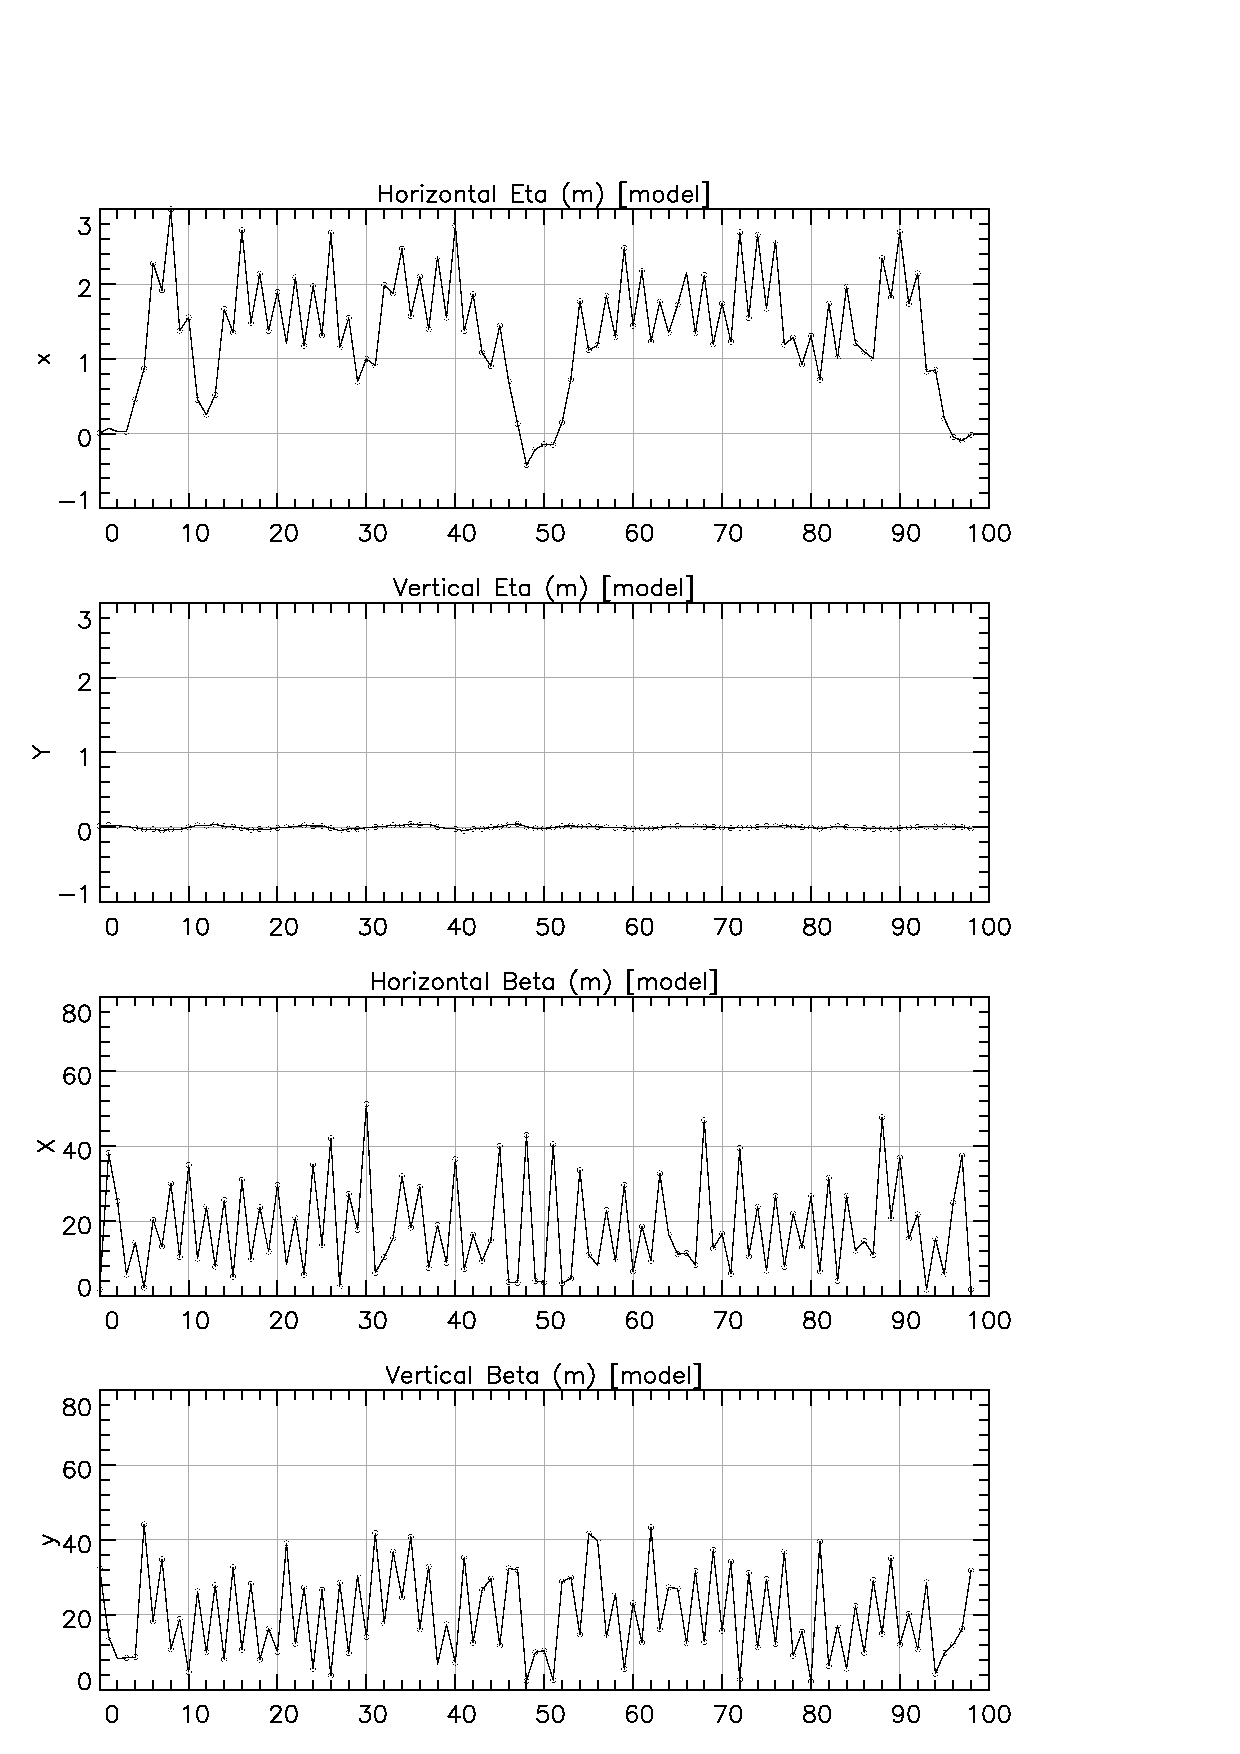
\includegraphics[width=5in]{plot_eta_beta.psfig}
  \caption{Plotting dispersion and beta function}
  \label{f:plot_eta_beta}
\end{figure}

\begin{figure}
  \centering
  \includegraphics[width=5in]{plot_coupling_no_IR.psfig}
  \caption{Zooming in on the residual coupling outside the IR.}
  \label{f:plot_coupling_no_IR}
\end{figure}

%----------------------------------------------------------------
\subsection{The \cmd{Show} Command}

Anything in the super-universe can be displayed using the \cmd{show}
command. To get a list of the data elements currently defined in \tao
type
\index{Commands!show}
\begin{example}
  show data
\end{example}
the output should look like:
\begin{example}
                                                              Bounds
     d2\_Name                       Ix  d1\_Name              Lower  Upper
     orbit
                                    1  x                      0    99
                                    2  y                      0    99
     phase
                                    1  x                      0    99
                                    2  y                      0    99
     eta
                                    1  x                      0    99
                                    2  y                      0    99
     beta
                                    1  x                      0    99
                                    2  y                      0    99
     cbar
                                    1  11                     0    99
                                    2  12                     0    99
                                    3  21                     0    99
                                    4  22                     0    99
     coupling
                                    1  11b                    0    99
                                    2  12a                    0    99
                                    3  12b                    0    99
                                    4  22a                    0    99

\end{example}
There are 6 data types defined in the initialization file. The fifth
and sixth are closely related. See Part II for an explanation of the
two coupling data types.  For the first four data types there are two
data dimensions defined corresponding to the horizontal and vertical
planes. Coupling is parameterized by a 2x2 matrix so there are four
``dimensions'' for these two data types. the ``Bounds'' columns refer
to the lower and upper indexes on the datums. there are 100 BPMs in
CESR so there are 100 data points.

To see the data values for the horizontal beta function for \cesr BPMs
1 through 50 type
\begin{example}
  show data beta.x[1:50]
\end{example}
Since we haven't changed any elements in the lattice yet the model
values equal the design values. Also note that \vn{beta.x} is actually
the a-mode betatron function. In regions with little or no coupling,
the a-mode is almost completely in the horizontal plane.

A significant point: The convention in \bmad is to label the twiss
parameters as \vn{x} and \vn{y} but they are actually the \vn{a} and
\vn{b} normal modes. So in regions of strong coupling \vn{beta.x} does
not correspond to \vn{orbit.x} which is always in the true horizontal
lab frame.  However, if you wish, you can re-label your twiss data
planes as \vn{a} and \vn{b}.  Section~\ref{c:init} shows you how to do
this. Keep in mind that lattice twiss parameters are defined
\textit{only for uncoupled betatron motion} so this is all that is
provided as data types for single particle tracking.  However, true
lab-frame \vn{x} and \vn{y} twiss parameters can be defined for a
distribution of particles so for particle or macroparticle beam
tracking true lab-frame \vn{x} and \vn{y} twiss parameters can be
calculated and are provided as data types for those tracking
types. See the \bmad manual for how to convert from normal mode
coordinates to lab-frame coordinates.

This tutorial uses single particle tracking and the twiss parameters
are found about the orbit of the tracked particle. there are two other
tracking types: particle beam and macroparticle beam tracking. these
tracking types will not be explored in this tutorial.

You can also view variables by typing
\begin{example}
  show var
\end{example}
To view the quadrupole k1 values for \cesr quadrupoles 5 and 20
through 30 type
\begin{example}
  sho var quad\_k1[5,20:30]
\end{example}
Again, since we haven't changed any quadrupoles the model values are
all at their design values.

You can also see the details of a particular lattice element. To view
the details for quadrupole Q05W type
\begin{example}
  sho ele Q05W
\end{example}

\vn{show var} and \vn{show ele} show two completely different types of
structures in \tao. Elements are the actual lattice elements as known
to \bmad.  Variables are native \tao structures that act kind of like
\bmad \textit{overlays} and only indirectly control the lattice
elements.

A list of lattice elements between two elements can be shown by typing 
\begin{example}
  sho lattice 0:20
\end{example}
This will show a list of all the lattice elements between and
including elements 0 and 20. Twiss parameters and orbit information at
each element is also provided.

Anything printed to the display using the \vn{show} command can also
be printed to a file by typing
\begin{example}
  show write <what_to_show>
\end{example}
\index{Commands!show}

A list of all intrinsic \vn{tao} commands can be found by typing
\index{Commands!help}
\begin{example}
  help
\end{example}
This will not list any custom commands. Detailed help on any
individual command can be found with
\begin{example}
  help <command\_name>
\end{example}
where \vn{<command_name>} is the command you want help with.

%----------------------------------------------------------------
%----------------------------------------------------------------
\section{Modifying the Lattice}
\label{s:modify_lattice}

\subsection{Changing a Variable}
\label{ss:change_variable}

Let's change a variable and see what happens to the lattice. We are going to
change a quadrupole strength so we should plot the change in beta and phase.
Type the following (everything after the `!' are just comments and can be
omitted):
\begin{example}
  x-axis all index        ! let the data index be the x-axis
  place top beta          ! plot Beta data on top plot
  place bottom phase      ! plot phase data on bottom plot
  plot all model - design ! plot the difference between model and design data
  scale                   ! scale all plots
\end{example}

The k1 value can be increased by 0.01 units for quadrupole Q05W by typing
\index{Commands!change}
\begin{example}
  change var quad\_k1 5 0.01
  scale
\end{example}
Note the information returned on the command line after the command
and the relative changes in beta and phase in the plot window. This is
a vertically focusing quadrupole so the vertical beta and phase is
affected more than the horizontal. The \cmd{0.01} at the end of the
command tells \tao to change this variable by 0.01 units. If you want
to set a variable to a particular value then use a ``@'' before the
value. So, to change this quadrupole k1 to -0.348 type
\begin{example}
  change var quad\_k1 5 @-0.348
\end{example}

\subsection{Putting things back where you found them}
\label{ss:put_it_back}

Let's put this quadrupole back where we found it. We can also modify
the quadrupole by modifying the lattice element directly by typing
\begin{example}
  change ele Q05W k1 d0.0
\end{example}
By modifying the element directly with the \cmd{change ele} command
you can modify almost any attribute of the element listed in the
output of \cmd{show ele Q05W}.  The ``d'' before the value is used to
set the variable relative to the design value.
\index{Commands!change}

If you've changed the lattice around a lot using variables, a great
way to set all variables back to their design values is to type
\index{Commands!set}
\begin{example}
  set var *|model = *|design
\end{example}
This only works if you just changed variables. If you changed any
elements directly with the \cmd{change ele} command then this will not
work. To set every attribute of every element back to the design type
\begin{example}
  set lattice model = design
\end{example}
Note that this will also recalculate the data and variable values
associated with the the model lattice to reflect the change so all the
bookkeeping is done for you.


%----------------------------------------------------------------
%----------------------------------------------------------------
\section{Running the Optimizer}\index{Optimization!running the optimizer}
\label{s:optimizer}

\index{lm!optimizer}\index{de!optimizer}
There are two non-linear optimizers included with \tao: Levenburg -
Marquardt, referred to as `\vn{lm}', and Differential Evolution, or
`\vn{de}'. This example will use the Levenburg - Marquardt optimizer
which first uses steepest decent to zero in on the region containing
the minimum then uses the inverse-Hessian to converge on the
minimum. See Numerical Recipes in Fortran (or C or C++) for a detailed
explanation. There's no need to know the details in order to use
either optimizer. Once you set up the problem \tao has the proper
wrapper routines to do the optimization. Of course, you are not
limited to using the included optimizers. Custom analysis can be done
using custom routines but these two optimizers have been integrated
`out of the box' with the \tao data and variable structures to make
quick optimization possible.

Basically, the `\vn{lm}' is typically faster since it uses a Jacobian
or ``dmerit'' matrix to find the data derivatives versus each variable
before starting the optimization process.  However it assumes the
second derivative is fairly smooth, so for very complex function
spaces the `\vn{de}' may work better. But because `\vn{lm}' typically
converges much faster (for functions it can handle) it is recommended
to try this one first and only use `\vn{de}' if it fails.

\subsection{Fix a Messed Up lattice}
\label{ss:fix_it}

Let's mess the lattice up a little and see if the optimizer can
``fix'' the lattice. First transfer the ``correct'' or \vn{design}
lattice to the \vn{meas} data area.
\begin{example}
  set data *.*|meas = *.*|design
\end{example}
Now mess up the lattice a bit. We'll be messing with quadrupoles so
plot beta and phase.
\begin{example}
  place top beta
  place bottom phase
  plot all meas - model
  change var quad\_k1 10 0.001
  change var quad\_k1 21 -0.001
  change var quad\_k1 67 -0.005
  scale
\end{example}
The lattice is now sufficiently screwed up.

Now specify what variables and data to use in the optimization. First type
\begin{example}
  show top10
\end{example}
to see what data is effecting the merit function the most. The merit
function is defined by
\Begineq
  {\cal M} \equiv \sum_{i} w_i \,
    \bigl[ \data_\model(i) -  \data_\meas(i) \bigr]^2 + 
  \sum_{j} w_j \,
    \bigl[ \var_\model(j) - \var_\meas(j) \bigr]^2
  \label{eq:merit}
\Endeq
where $w_{i}$ and $w_{j}$ are the weights given to each component.
The optimizer tries to minimize the merit function by changing the
model to look like the measured data. From the \vn{top10} output we
see that the beta function is effecting the merit function the
most. Since we are looking at beta and phase let's only use that data
in the optimization.
\begin{example}
  veto data *
  use  data beta
  use  data phase
\end{example}
We also know that we need to change quadrupoles to correct the lattice.
\begin{example}
  veto var *          ! veto all the data
  restore var quad\_k1 ! restore just the quad\_k1 data
\end{example}
Note that we need to specify what data and variables we will be using
beforehand in the initialization files. This is already taken care of
in the demo initialization files. You can view these files to see how
the data and variables were initialized. Raw lattice elements cannot
be used by the included optimizer but there is no such restriction on
custom optimizers.

Now let's see if we have the optimizer set up correctly.
\begin{example}
  sho optimizer
\end{example}
Whoops! we want to use the Levenburg - Marquardt optimizer so
\begin{example}
  set global optimizer = lm
  sho opt
\end{example}
The second command is short-hand. Most \tao commands can be shortened
to the least number of characters needed to distinguish the command
from all others.

Now we're ready to run the optimizer or ``fit'' the model to the
`measured' data.
\begin{example}
  run
\end{example}
You see the optimizer going through its cycles and it did it! The
model is now ``fitted.'' We can see what changes where done to the
quadrupoles by typing
\begin{example}
  sho var quad\_k1
\end{example}
The optimizer came very close to finding the ``design''
lattice. However, it changed more quadrupoles than just 10, 21 and
67. This isn't surprising. The optimizer finds the minimum of the
merit function and there are potentially many minimums, or
degeneracies.  It does it's best not to get stuck in a local minimum
and as we can see by the plotted data, the minimum found is very close
-- virtually identical -- to the design lattice optics.  A good hint
as to what variables will be adjusted is the output of \cmd{show
top10}.  The top 3 derivatives were not the quadrupoles we
adjusted. Nevertheless, the final result was a darn near perfect
match!

\subsection{Now Not Using all of the Variables}
\label{ss:fix_it_not_all}

Alternatively, we could have used only a subsection of the
quadrupoles. Say we know approximately which quadrupoles should be
adjusted. We can then specify these variables ranges.
\begin{example}
  change var quad\_k1[10]   0.001
  change var quad\_k1[21]  -0.001
  change var quad\_k1[67]  -0.005
  scale
  use var quad\_k1[8:12,20:25,65:70]
  run
  sho var quad\_k1[8:12,20:25,65:70]
\end{example}
Different quadrupoles than the ones we initially changed were still
adjusted by the optimizer. The end result is again very close to the
design lattice.

\subsection{Lattice Design}
\label{ss:lattice_design}

You may wish to constrain beam parameters instead of ``fitting'' to
data. For example, you could want the beta function not to exceed a
value in a certain part of the machine. \tao will also perform this
type of optimization.

\fbox{this subsection is yet to be completed!} 

%----------------------------------------------------------------
%----------------------------------------------------------------
\section{Single Mode}\index{Single Mode}
\label{s:single_mode}

Single mode utilizes a simple single character interface to the \tao
model lattice.  By simply typing single predefined characters the
specified element parameter will be changed by a certain amount. This
allows the user to quickly converge on a neighborhood around the
minimum of a multidimensional non-linear function space. However,
finding the exact minimum can be difficult to do by hand. Once the
neighborhood is found the optimizer can be used to narrow in on the
optimum configuration without requiring it to run all around the
parameter space, which is very inefficient and time consuming for
complex parameter spaces.

\fbox{this section is yet to be completed!} 

%----------------------------------------------------------------
%----------------------------------------------------------------
\section{Where to go from here}
\label{s:where_to_go}

You now have an understanding of the basic abilities of \tao. After
this tutorial, Part II of the \tao Manual should be legible and
useful.  The Reference Guide will provide the details of everything
mentioned in this tutorial.  It goes into detail of setting up your
own initialization files and how to use the optimizer. It also
includes a complete command reference with command syntax.

However, you're not yet ready to customize \tao, but this is where the
true versatility of \tao lies. So, onward to the next section and
learn how to write your own custom routines to perform whatever
accelerator calculations that strikes your fancy!

%----------------------------------------------------------------
%----------------------------------------------------------------
%----------------------------------------------------------------
%----------------------------------------------------------------
\chapter{Customizing Tao}\index{Customizing}
\label{c:custom_tao}

%----------------------------------------------------------------
\section{It's all a matter of Hooks}\index{Customizing!Hooks}

The golden rule when extending \tao is that you are only allowed to
replace routines or redefine structures that have the name ``hook'' in
them.  If you have the source code then it's within your power to
modify any routine in \tao as much as you like. However, as time goes
by, and revisions are made to the \tao routines to extend the
usefulness of \tao and to eliminate bugs, only modifying the ``hook''
routines will ensure that custom changes will have a minimum impact on
the specialized routines that will be written by various people.

\tao is written in Fortran 95 and a knowledge of Fortran is
required. However, if you know C then Fortran can be learned in a
coupled of days. Because of the interoperability between C and Fortran
once the wrapper routines are written to interface with \tao the rest
of your coding can, in principle all be done in C.

\tao relies on extensive use of pointers and logical flags. However,
all of the structures you will need to use are contained in the
\vn{tao_struct.f90} module. This module is heavily documented and
provides all the information needed to use the intrinsic \tao
structures on your customizations. It is also a very good idea to have
a copy of \vn{bmad_struct.f90} handy as this contains most of the
structures used by \bmad.

%----------------------------------------------------------------
\section{Compiling your custom Tao}
\index{Customizing!Compiling}

The \tao libraries can be compiled without compiling an
executable. Here is where this comes in handy. Since the standard \tao
subroutines have already been made into libraries, all you need to do
is compile and link your custom routines with the standard \tao
subroutines into an executable.

There are 11 ``hook'' files located in the \cmd{ROOT/tao/hook}
directory. These are the files you can customize. There are two
options here.
\begin{enumerate}
  \item Change the files directly in \cmd{ROOT/tao/hook}, adding any extra
    files you may need, then recompile from the \cmd{ROOT/tao} directory with
  \cmd{gmake -f M.tao}.  \label{cust_option_one}
  \item Copy the hook files to a separate directory say \cmd{ROOT/my_tao},
    adding any extra files you may need, then write a Makefile to 
    compile and link these
    routines to the main \tao library. \label{cust_option_two}
\end{enumerate}
Option~\ref{cust_option_two} is HIGHLY recommended because it keeps
the \tao distribution tree undisturbed and reserves the possibility to
create multiple custom \tao programs using the same vanilla \tao
library. This option is used in the following example.

%----------------------------------------------------------------
\section{An Example}\index{Customizing!Example}

As an example let's include a new data type called
\vn{particle_emittance}. This will be the non-normalized x and y
emittance as found from the Courant-Snyder invariant. This data type
will behave just like any other data type (i.e.  \vn{orbit},
\vn{phase} etc...). First, we should copy all the hook files to a
separate directory, call it \cmd{ROOT/my_tao}. Also include the main
program file from the \cmd{ROOT/tao/program} directory.  (replace
\vn{ROOT} with whatever top directory you placed the \vn{tao}
directory.)
\begin{example}
  mkdir ROOT/my_tao
  cp ROOT/tao/hook/*.f90 ROOT/my_tao
  cp ROOT/tao/program/tao_cl.f90 ROOT/my_tao/my_tao_cl.f90
\end{example}
Next we need a Makefile. The \cmd{ROOT/tao/M.tao} 
Makefile is a great starting point.
\begin{example}
  cp ROOT/tao/M.tao ROOT/my_tao/Makefile
\end{example}
Now change the following lines in your Makefile
\begin{example}
  LIB\_SRC\_DIRS := ./code ./hook
  OBJ\_SRC\_DIRS := ./program
\end{example}
to
\begin{example}
  LIB\_SRC\_DIRS :=
  OBJ\_SRC\_DIRS := ./
\end{example}
This Makefile will tell gmake to use the tao library that has already
been created (from \cmd{../tao/code} but the actual library is located
at \cmd{../lib/libtao.a})
 and then to compile
all of the hook files, including the main program file
(\cmd{my_tao_cl.f90}) into object files (everything in \cmd{./}, the
current directory).  Routines and declarations in object files always
override similarly named code in the \tao libraries so this allows for
your local hook files to override the dummy hook files in the \tao
library. The only downside to this method is it clutters your
\cmd{my_tao} directory with object files. You can always remove these
object files with \cmd{gmake clean}.

There are two more lines to alter. change
\begin{example}
  MAIN\_FILE :=
\end{example}
to
\begin{example}
  MAIN\_FILE := ./my\_tao_cl.f90
\end{example}
and finally,
\begin{example}
  MAKEFILE := M.tao
\end{example}
to
\begin{example}
  #MAKEFILE := M.tao !using default name for Makefile
\end{example}
Notice that this line is just being commented out with a `\#'. You are
now ready to make your customizations to the hook routines.

This example will only require the modification of one file:
\vn{tao_hook_load_data_array.f90}. The formula for single particle emittance is
\Begineq
  \epsilon = \gamma x^{2} + 2 \alpha x x' + \beta x'^{2}
  \label{e:emittance}
\Endeq
Place the following code in \vn{tao_hook_load_data_array.f90} in the
\cmd{case select} construct (also add the necessary type declarations)
\begin{verbatim}
  case ('particle_emittance:x') 

    datum_value =  ( ele%x%gamma * orb(ix1)%vec(1)**2 + &
		     2 * ele%x%alpha * orb(ix1)%vec(1) * orb(ix1)%vec(2) + &
		     ele%x%beta * orb(ix1)%vec(2)**2)
    
  case ('particle_emittance:y')

    datum_value = ( ele%y%gamma * orb(ix1)%vec(3)**2 + &
		     2 * ele%y%alpha * orb(ix1)%vec(3) * orb(ix1)%vec(4) + &
		     ele%y%beta * orb(ix1)%vec(4)**2)
\end{verbatim}
This defines what is to be calculated for each \vn{particle_emittance}
datum.  There are two transverse coordinates, so two definitions need
to be made, one for each dimension.

Now you just need to declare the data types in the \cmd{tao.init} and
\cmd{tao_plot.init} files. For the sake of this example, modify the
initialization files used for this tutorial.
\begin{example}
  cp ROOT/tao/program/*.init ROOT/my_tao
  cp ROOT/tao/program/*.lat ROOT/my_tao
\end{example}

In \cmd{ROOT/my_tao/tao.init} add the following lines to the data
declarations section
\begin{example}
  &tao_d2_data
    d2_data%name = "particle_emittance" 
    universe = 0 
    n_d1_data = 2
  /

  &tao_d1_data
    ix_d1_data = 1
    d1_data%name = "x"  
    default_weight = 1
    ix_min_data = 0 
    ix_max_data = 99  
    data(0)%name = "SAME: orbit.x"
    data(0)%ele_name = "SAME: orbit.x"
  /

  &tao_d1_data
    ix_d1_data = 2
    d1_data%name = "y"  
    default_weight = 1
    ix_min_data = 0 
    ix_max_data = 99  
    data(0)%name = "SAME: orbit.x"
    data(0)%ele_name = "SAME: orbit.x"
  /
\end{example}
and increase \vn{n_d2_data_max} to 7 in the \vn{tao_params} declaration.

In \cmd{ROOT/my_tao/tao_plot.init} add the following lines to the end
of the file
\begin{example}
  &tao_template_plot
    plot%name = 'particle_emittance'
    plot%x%min =   0
    plot%x%max = 100
    plot%x%major_div = 10
    plot%x%label = ' '
    plot%x_axis_type = 'index'
    plot%n_graph = 2
  /
  
  &tao_template_graph
    graph%name = 'x'
    graph_index = 1
    graph%box = 1, 2, 1, 2
    graph%title = 'Horizontal Emittance (microns)'
    graph%margin =  0.15, 0.06, 0.12, 0.12, '%BOX'
    graph%y%label = 'x'
    graph%y%max =  15
    graph%y%min =  0.0
    graph%y%major_div = 4
    graph%n_curve = 1
    curve(1)%data_source = 'data_array'
    curve(1)%data_type   = 'particle_emittance:x'
    curve(1)%y_axis_scale_factor = 1e6 !convert from meters to microns
  /

  &tao_template_graph
    graph%name = 'y'
    graph_index = 2
    graph%box = 1, 1, 1, 2
    graph%title = 'Vertical Emittance (microns)'
    graph%margin =  0.15, 0.06, 0.12, 0.12, '%BOX'
    graph%y%label = 'Y'
    graph%y%max =  15
    graph%y%min =  0.0
    graph%y%major_div = 4
    graph%n_curve = 1
    curve(1)%data_source = 'data_array'
    curve(1)%data_type = 'particle_emittance:y'
    curve(1)%units_factor = 1e6 !convert from meters to microns
  /
\end{example}
These namelists are described in detail in Chapter~\ref{c:init}.

We are now ready to compile and then run the program. The \tao library
should have already been created (in section~\ref{s:get_and_compile})
so all you need to do is
\begin{example}
  cd ROOT/my_tao
  gmake
  ../bin/my_tao_cl
\end{example}
Notice that the name of the custom \tao program is \cmd{my_tao_cl}. If you run 
`\cmd{../bin/tao}' then you will run ``vanilla'' \tao.

After your custom \tao initializes type
\begin{example}
  place bottom particle_emittance
  scale
\end{example}
Your plot should look like Figure~\ref{f:plot_emittance}.

The emittance (as calculated) is not constant. This is due to
dispersion and coupling throughout the ring. \bmad provides a routine
to find the particle emittance from the twiss parameters that includes
dispersion and coupling called \vn{orbit_amplitude_calc}.

\begin{figure}
  \centering
  \includegraphics[width=5in]{plot_emittance.psfig}
  \caption{Custom data type: non-normalized emittance}
  \label{f:plot_emittance}
\end{figure}

\Section{Other Customizations}

The above example just illustrates one of the customizations you can
perform on \tao.  Part III, Programmer's Guide lays out all of the
hook files and provides pointers for various customizations.



\part{Reference Guide}\label{ref_guide}

\chapter{Data types}
\label{c:data_types}

%------------------------------------------------------------------------
\section{How Tao Handles Data}\index{Data}

As explained in chapter~\ref{c:overview}, \tao has special structures to hold
data to be analyzed. Any lattice or beam parameters that are needed to be
analyzed or plotted must have a data type defined for it. In general, a data
type can be any type of parameter that is not necessarily measurable in a real
world machine. For example, there is an orbit data type and a BPM data type. The
orbit data is the real x,y,z position of a particle in the lab frame whereas the BPM
data is the x and y reading on a simulated beam position monitor that includes
any offsets, tilts and noise.

\tao includes many different data types already predefined and
these can be classified into three main catagories:
\begin{enumerate}
  \item \textbf{Lattice Parameters} \Newline
    For example lattice twiss parameters, coupling and floor position.
  \item \textbf{Single Particle Properties} \Newline
    For example particle orbit, BPM reading and phase advance.
  \item \textbf{Bunch Properties} \Newline
    For example bunch sigmas, emittance and beam twiss parameters.
\end{enumerate}
For a given data type the method used to calculate the datum can vary depending
on the tracking type. For {\it single} particle tracking all data is found from
the lattice parameters except for the orbit data. For \textit{particle bunch} or
\textit{macroparticle bunch} tracking some of the datums  are found from the
particle distribution using the appropriate \bmad routines. For example, with
single particle tracking the beta function is found from the lattice transport
matrix, however, with particle or macroparticle tracking the beta function is
found from the particle distribution using the formula
\begin{equation}
  \beta = \frac{<x^{2}>}{\sqrt{<x^{2}> <x'^{2}> - <x x'>^{2}}}.
\end{equation}
The next section will describe how each predefined data type is calculated.
Custom data types need not fall into one of the above catagories and can be any
real number as calculated in the appropriate hook routine.

Also associated with a datum are two lattice elements called
\vn{ele} and \vn{ele2}. The \vn{data_types} are divided into two
categories: Those that are \vn{relative} and those that are not.  A
\vn{relative} \vn{data_type} means that the \vn{model} value for that
datum is determined by a difference between elements. For example, for
\vn{phase:x} the \vn{model} value is
\begin{example}
  model_value = \(\phi\sb{x}\)(ele) - \(\phi\sb{x}\)(ele2)
\end{example}
If there is no \vn{ele2} associated with a datum then the model value is
\begin{example}
  model_value = \(\phi\sb{x}\)(ele) - \(\phi\sb{x}\)(0)
\end{example}
where $\phi_x(0)$ is the phase at the 0\Th element (which is always at 0 radians).
\index{Data!Relative}

For datums with \vn{non-relative} \vn{data_types} if there is also an
associated \vn{ele2} element then the \vn{model} value is dependent
upon the \vn{merit_type}. For example, with a \vn{beta:x} \vn{data_type} the
model value is determined by Table~\ref{t:eval2} where \vn{i} goes from the
\vn{ele} index to the \vn{ele2} index.
\begin{table}[ht]
\centering
{\tt
\begin{tabular}{|l|l|l|} \hline
  {\it Merit\_Type}       & {\it Model Value} \\ \hline 
  \vn{min}     & $\min \beta_x(i)$ \\ \hline 
  \vn{max}     & $\min \beta_x(i)$ \\ \hline 
  \vn{abs_min} & $\min |\beta_x(i)|$ \\ \hline 
  \vn{abs_max} & $\min |\beta_x(i)|$ \\ \hline 
  \vn{target}  & {\it Error}   \\ \hline 
\end{tabular}
}
\caption{\vn{Model} evaluation.}
\label{t:eval2}
\end{table}

%------------------------------------------------------------------------
\section{Tao Data Types}\index{Data!Data Types}
\label{s:data_types}

Table~\ref{t:data_types} lists the predefined data types in \tao.
Table~\ref{t:data_calc_method} lists how each data type is calculated depending
on the tracking type. A ``L'' means that the lattice determines the data type.
In \bmad the twiss parameters are calculated about a reference orbit so the
centroid orbit (or particle orbit for single particle tracking) is also used.
A ``B'' means the beam particle distribution determines the data type. A ``X''
means this data type is not available for this tracking type.
\index{Data!Calculation Method}

\begin{table}[ht] 
\centering 
{\tt
\begin{tabular}{|l|l|l|} \hline
  {\it Data\_Type}        & {\it Description}                 &          \\ \hline 
    beta:x, beta:y        & Projected Beta Function           &          \\ \hline 
    beta:a, beta:b        & Normal-Mode Beta Function         &          \\ \hline 
    alpha:x, alpha:y      & Projected Alpha Function          &          \\ \hline 
    alpha:a, alpha:b      & Normal-Mode Alpha Function        &          \\ \hline 
    eta:x, eta:y          & Dispersion                        &          \\ \hline 
    etap:x, etap:y        & Dispersion derivative             &          \\ \hline 
    phase:x, phase:y      & Betatron phase                    & relative \\ \hline 
    orbit:x, orbit:y      & Transverse orbit                  &          \\ \hline 
    orbit:p\_x, orbit:p\_y& Tranverse momenta                 &          \\ \hline 
    orbit:z, orbit:z\_p   & Longitudinal orbit and momenta    &          \\ \hline 
    bpm:x, bpm:y          & Transverse BPM reading            &          \\ \hline 
    \begin{tabular}{@{}l}     
      cbar:11, cbar:12, \\ 
      cbar:21, cbar:22 
    \end{tabular} 
                          & Coupling                         &          \\ \hline 
    \begin{tabular}{@{}l}   
      coupling:11b, coupling:12a, \\ 
      coupling:12b, coupling:22a 
    \end{tabular} 
                          & Coupling                         &          \\ \hline 
    floor:x, floor:y, floor:z
                          & Global (``floor'') position      & relative \\ \hline 
    floor:theta           & Global (``floor'') angle         & relative \\ \hline 
    r:$ij$                & 
                           \begin{tabular}{l}
                             Term in linear transfer map \\
                             $1 \le i,j \le 6$
                           \end{tabular}
                                                             & relative \\ \hline 
    t:$ijk$               & 
                           \begin{tabular}{l}
                             Term in 2\Nd order transfer map \\
                              $1 \le i,j,k \le 6$
                           \end{tabular} 
                                                             & relative \\ \hline 
    tt:$ijklm\ldots$      & 
                           \begin{tabular}{l}
                             Term in n\Th order transfer map \\
                              $1 \le i,j,k,\ldots \le 6$
                           \end{tabular} 
                                                              & relative \\ \hline 
    i5a\_e6, i5b\_e6      & Normalized I5 radiation integral  &          \\ \hline
    s\_position           & longitudinal length constraint    & relative \\ \hline 
    beam\_energy          & Beam energy                       &          \\ \hline
    \begin{tabular}{@{}l}  
      norm\_emittance:x \\ 
      norm\_emittance:y \\
      norm\_emittance:z \\
      norm\_emittance:a \\
      norm\_emittance:b \\
    \end{tabular} 
                          & Normalized emittance              &          \\ \hline 
    \begin{tabular}{@{}l}   
      bunch\_sigma:x, bunch\_sigma:p\_x \\ 
      bunch\_sigma:y, bunch\_sigma:p\_y \\
      bunch\_sigma:z, bunch\_sigma:p\_z \\
    \end{tabular} 
                          & Bunch size                        &          \\ \hline 
    \begin{tabular}{@{}l}  
      dpx\_dx \\ 
      dpy\_dy \\
      dpz\_dz \\
      dpa\_da \\
      dpb\_db \\
    \end{tabular} 
                          & <x p\_x> / <x\^2> \& Etc...       &          \\ \hline 
\end{tabular}
} 
\label{t:data_types}
\caption{Predefined Data Types}
\end{table}

\vfill \break
{\vfill}

\index{Element!table of data calculation methods}
\begin{table}[ht] 
\centering {
\begin{tabular}{|l|c|c|c|} \hline
\rule{0pt}{80pt} 
\vn{Data_Type}       &
\begin{sideways}\vn{Single}\end{sideways} &
\begin{sideways}\vn{Particle Beam}\end{sideways} &
\begin{sideways}\vn{Macroparticle Beam}\end{sideways} 
\\ \hline
%   data type             & Single & Beam & Macroparticle
    \vn{beta}             &   L    &   B  &   B   \\ \hline
    \vn{alpha}            &   L    &   B  &   B   \\ \hline
    \vn{eta}              &   L    &   B  &   B   \\ \hline
    \vn{etap}             &   L    &   B  &   B   \\ \hline
    \vn{phase}            &   L    &   L  &   L   \\ \hline
    \vn{orbit}            &   B    &   B  &   B   \\ \hline
    \vn{bpm}              &   B    &   B  &   B   \\ \hline
    \vn{cbar}             &   L    &   L  &   L   \\ \hline
    \vn{coupling}         &   L    &   L  &   L   \\ \hline
    \vn{floor}            &   L    &   L  &   L   \\ \hline
    \vn{r}                &   L    &   L  &   L   \\ \hline
    \vn{t}                &   L    &   L  &   L   \\ \hline
    \vn{tt}               &   L    &   L  &   L   \\ \hline
    \vn{i5a_e6, i5b_e6}   &   L    &   L  &   L   \\ \hline      
    \vn{s_position}       &   L    &   L  &   L   \\ \hline           
    \vn{beam_energy}      &   L    &   L  &   L   \\ \hline  
    \vn{norm_emittance}   &   L\footnote{Uses the Courant-Snyder Invariant}    &   B  &   B   \\ \hline
    \vn{bunch_sigma}      &   X    &   B  &   B   \\ \hline
    \vn{dpx_dx,dpy_dy,...}&   X    &   B  &   B   \\ \hline
\end{tabular}
}
\caption{Data\_type Calculation method. L means this data type uses lattice parameters, B
means this data type uses beam parameters. X mean this data is unavailable for
this tracking type.}
\label{t:data_calc_method}
\end{table}

\vfill\break


\chapter{Optimization}
\label{c:opti}

%------------------------------------------------------------------------
\section{Lattice Corrections}

Examples of lattice corrections include flattening the orbit and
adjusting quadrupoles to correct the measured betatron phase. The
general idea is to vary an appropriate set of \vn{variables} with the
aim of minimizing a merit function \vn{M} that is a measure of how
well \vn{data_model}, the data as calculated from the \vn{model} fits
\vn{data_meas}, the measured data
\Begineq
  {\cal M} \equiv \sum_{i} w_i \,
    \bigl[ \data\_\model(i) -  \data\_\meas(i) \bigr]^2 + 
  \sum_{j} w_j \,
    \bigl[ \var\_\model(j) - \var\_\meas(j) \bigr]^2
  \label{m1}
\Endeq
\vn{var_model} is the value of a variable in the \vn{model} and
\vn{var_meas} is the value as measured at the time the data was taken
and the sum \vn{j} runs over all variables that are allowed to be
varied to minimize \vn{M}. The second term in the merit function
prevents degeneracies (or near degeneracies) in the problem which
would allow \tao to find solutions where \vn{data_model} matches
\vn{data_measured} with the \vn{var_model} having ``unphysical''
values (values far from \vn{var_meas}. The weights $w_i$ and $w_j$
need to be set depending upon how accurate the measred data is
relative to how accurate the calibrations for measuring the
\vn{var_meas} values are. With the second term in the merit function
the number of constraints (number of terms in the merit function) is
always larger than the number of variables and degeneracies can never
occur. 

The algorithm used to vary the \vn{var_model} variables to minimize
\vn{M} is called an \vn{optimizer}. In \vn{command line mode} the
\vn{run} command is used to invoke an \vn{optimizer}. In \vn{single
mode} the \vn{g} key starts an optimizer and the \vn{.} key stops it.
Running an optimizer is also called ``fitting'' since one is trying to
get the \vn{data_model} to be equal to the \vn{data_meas}. With orbits
this is also called ``flattening'' since one generally wants to end up
with an orbit that is on--axis.

In a correction one wants to change the machine variables so that the
measured data corresponds to the design values \vn{data_design}. Thus
the change in the data that one wants is
\begin{example}
  data_change = data_design - data_meas
\end{example}
Once a fit has been made, and presuming that the \vn{data_model} is
resonably close to the \vn{data_meas} this data change within the
\vn{model} lattice can be accomplished by changing the variables by
\begin{example}
  var_change = var_design - var_model
\end{example}
This assumes the system is linear. For many situations this is true
since typically \vn{var_change} is ``small''. Since the variables have
a measured value of \vn{var_meas} the value that the variables should
be set to is
\begin{example}
  var_final = var_meas + (var_design - var_model)
\end{example}
Notice that the fitting process is independent of the \vn{design}
lattice. It is only when calculating the corrections to the
variables that the \vn{design} lattice plays a roll. 

Sometimes it is desired to fit to changes in data as opposed to the
absolute value of the data. For example, when closing an orbit bump
knob what is important is the difference in orbits before and after
the bump knob is varied. Designating one of these orbit the
\vn{reference}, the appropriate merit function is
\begin{alignat}{1}
  {\cal M} = &\sum_{i} w_i \,
    \Bigl[ \bigl( \data\_\model(i) - \data\_\design(i) \bigr) - 
      \bigl( \data\_\meas(i) - \data\_\reference(i) \bigr) \Bigr]^2 + \CRNO
  &\sum_{j} w_j \,
    \Bigl[ \bigl( \var\_\model(j) - \var\_\design(j) \bigr) -
     \bigl( \var\_\meas(i) - \var\_\reference(i) \bigr) \Bigr]^2 
  \label{m2}
\end{alignat}
where \vn{data_ref} and \vn{var_ref} refer to the reference
measurement.  This merit function is acceptable if the reference data
is taken with the machine reasonably near the design setup so that
nonlinearities can be ignored. If this is not the case then the
fitting becomes a two step process: The first step is to fit the
\vn{model} to the \vn{reference} data using the merit function of
\Eq{m1}. The \vn{base} lattice is then set equal to the \vn{model}
lattice. The second step is to fit the model using the merit function
\begin{alignat}{1}
  {\cal M} = &\sum_{i} w_i 
    \Bigl[ \bigl( \data\_\model(i) - \data\_\base(i) \bigr) - 
      \bigl( \data\_\meas(i) - \data\_\reference(i) \bigr) \Bigr]^2 + \CRNO
  &\sum_{j} w_j 
    \Bigl[ \bigl( \var\_\model(j) - \var\_\base(j) \bigr) -
     \bigl( \var\_\meas(i) - \var\_\reference(i) \bigr) \Bigr]^2 
  \label{m3}
\end{alignat}

Control of what data and what variables are to be used in the fitting
process is controlled by the \vn{use}, \vn{veto}, \vn{restore}, and
\vn{clip} commands.

%------------------------------------------------------------------------
\section{Lattice Design}

Lattice design is the process of calculating \vn{variable} strengths
to meet a number of criteria called constraints. For example, one
constraint could be that the beta function in some part of the lattice
not exceed a certain value. In this case we can proceed as was done
for lattice correction and define a merit function to be minimized:
\Begineq
  {\cal M} = \sum_{i} w_i \, C_i^2
\Endeq
Typically constraints are either to limit values to some range so the
constraint would be of the form
\Begineq
  C = 
    \begin{cases}
    \mbox{model} - \mbox{limit}  & \mbox{model $>$ Limit} \\
    0                            & \mbox{otherwise}
    \end{cases}
\Endeq
or a constraint is used to keep the \vn{model} at a certain value so
the form of the constraint would be
\Begineq
  C = \mbox{model} - \mbox{target}  
\Endeq
Here \vn{model} is the value as calculated from the \vn{model}
lattice. \vn{target} and \vn{limit} are given numbers. Part of the
optimization process is in deciding what the values should be for any
\vn{target} or \vn{limit}.

%------------------------------------------------------------------------
\section{Generalized Design}

Since lattice design and lattice corrections are similar, \tao
combines the two into one generalized correction process. In this
generalized process The merit function becomes
\Begineq
  {\cal M} = \sum_i w_i \, D_i^2 + \sum_j w_j \, V_j^2
\Endeq
The general form of the data merit terms $D_i$ is 
\Begineq
  D = 
    \begin{cases}
    \mbox{delta}  & \mbox{Non-zero Condition} \\
    0             & \mbox{Otherwise}
    \end{cases}
\Endeq
The \vn{Non-zero Condition} needed for a non--zero $C_i$ is dependent
upon the \vn{merit_type} of the datum. There are five constraint
types as given in Table~\ref{t:con_type}.
\begin{table}[h]
\centering
{\tt
\begin{tabular}{|l|l|l|} \hline
  {\it Merit\_Type}       & {\it Non-zero Condition} \\ \hline 
  \vn{target}            & Any \vn{delta}   \\ \hline 
  \vn{min}, \vn{abs_min} & \vn{delta} $<$ 0 \\ \hline 
  \vn{max}, \vn{abs_max} & \vn{delta} $>$ 0 \\ \hline 
\end{tabular}
}
\caption{Constraint Type List.}
\label{t:con_type}
\end{table}

The form of \vn{delta} is determined by two global logicals called
\vn{opt_with_ref} and \vn{opt_with_base} as shown in
Table~\ref{t:d_i}. 
\begin{table}[h] 
\centering 
{\tt
\begin{tabular}{|l|l|l|} \hline
  \vn{Opt_with_ref} & \vn{Opt_with_base} & \vn{delta} \\ \hline 
  F & F & Model - Meas                \\ \hline 
  T & F & Model - Meas + Ref - Design \\ \hline 
  F & T & Model - Meas - Base         \\ \hline 
  T & T & Model - Meas + Ref - Base   \\ \hline 
\end{tabular}
} 
\caption{$D_i$ Form}  
\label{t:d_i}
\end{table}

What kind of data is associated with \vn{model}, \vn{design} and
\vn{base} is determined by a datum's \vn{data_type}. Valid
\vn{data_types} are given in table~\ref{t:cons}.
\begin{table}[h] 
\centering 
{\tt
\begin{tabular}{|l|l|l|} \hline
  {\it Data\_Type} & {\it Description}        &          \\ \hline 
    beta:x, beta:y    & Twiss parameter                 &          \\ \hline 
    alpha:x, alpha:y  & Twiss parameter                 &          \\ \hline 
    eta:x, eta:y      & Dispersion                      &          \\ \hline 
    etap:x, etap:y    & Dispersion derivative           &          \\ \hline 
    phase:x, phase:y  & Betatron phase                  & relative \\ \hline 
    orbit:x, orbit:y  & Particle orbit                  &          \\ \hline 
\begin{tabular}{@{}l}     cbar:11, cbar:12, \\ cbar:21, cbar:22 \end{tabular} 
                      & Coupling                        &          \\ \hline 
\begin{tabular}{@{}l}     coupling:11b, coupling:12a, \\ 
                          coupling:12b, coupling:22a \end{tabular} 
                      & Coupling                        &          \\ \hline 
    floor:x, floor:y, floor:z
                      & Global (``floor'') position     & relative \\ \hline 
    floor:theta       & Global (``floor'') angle        & relative \\ \hline 
    r56               & Term in linear transfer map     & relative \\ \hline 
    t566              & Term in 2nd order transfer map  & relative \\ \hline 
    i5a\_e6, i5b\_e6  & Normalized I5 radiation integral &          \\ \hline
    s\_position       & longitudinal length constraint  & relative \\ \hline 
    beam\_energy      & Beam energy                     &          \\ \hline
\end{tabular}
} 
\caption{Constraint List.}
\label{t:cons}
\end{table}

Also associated with a datum are one or two lattice elements called
\vn{ele} and \vn{ele2}. The \vn{data_types} are divided into two
categories: Those that are \vn{relative} and those who are not.  A
\vn{relative} \vn{data_type} means that the \vn{model} value for that
datum is determined by a difference between elements. For example, for
\vn{phase:x} the \vn{model} value is
\begin{example}
  model_value = \(\phi\sb{x}\)(ele2) - \(\phi\sb{x}\)(ele)
\end{example}
If there is no \vn{ele2} associated with a datum then the model value is
\begin{example}
  model_value = \(\phi\sb{x}\)(ele) - \(\phi\sb{x}\)(0)
\end{example}
where $\phi_x(0)$ is the phase at the 0\Th element (which is always 0).

For datums with \vn{non-relative} \vn{data_types} If there is also an
associated \vn{ele2} element then the \vn{model} value is dependent
upon the \vn{merit_type}. For example, with a \vn{beta:x} \vn{data_type} the
model value is determined by Table~\ref{t:eval}.
\begin{table}[h]
\centering
{\tt
\begin{tabular}{|l|l|l|} \hline
  {\it Merit\_Type}       & {\it Model Value} \\ \hline 
  \vn{min}     & $\min_{\mbox{ele} \le i \le \mbox{ele2}} \beta_x(i)$ \\ \hline 
  \vn{max}     & $\min_{\mbox{ele} \le i \le \mbox{ele2}} \beta_x(i)$ \\ \hline 
  \vn{abs_min} & $\min_{\mbox{ele} \le i \le \mbox{ele2}} |\beta_x(i)|$ \\ \hline 
  \vn{abs_max} & $\min_{\mbox{ele} \le i \le \mbox{ele2}} |\beta_x(i)|$ \\ \hline 
  \vn{target}  & {\it Error}   \\ \hline 
\end{tabular}
}
\caption{\vn{Model} evaluation.}
\label{t:eval}
\end{table}

The form of the variable terms $V_i$ is determined by its \vn{merit_type}.
For variables the merit types are:
\begin{example}
  target
  limit
\end{example}
A \vn{target} \vn{merit_type} for a variable is the same as for
datum. In this case \vn{model} is just the value of the variable.
A \vn{limit} \vn{merit_type} has the form
\Begineq
  V = 
    \begin{cases}
    \mbox{model} - \mbox{high\_lim}  & \mbox{model} > \mbox{high\_lim} \\
    \mbox{model} - \mbox{low\_lim}   & \mbox{model} < \mbox{low\_lim} \\
    0                               & \mbox{Otherwise}
    \end{cases}
\Endeq

Note: when doing lattice design \vn{opt_with_ref} and
\vn{opt_with_base} are both set to \vn{False} and the \vn{target} and
\vn{limit} values are identified with \vn{Meas}.




\chapter{Tao Initialization}
\index{Initialization}
\label{c:init}

\tao is customized for specific machines and specific calculations using input files and custom
software routines. Writing custom software is covered in the programmer's guide section. This
chapter covers the input files.

In general, the input files tell \tao:
\begin{example}
  * What \bmad lattice or lattices to use (\sref{s:init.lat}).
  * What the variables and data should be when running optimizations (\sref{c:opti}).
  * What to plot and how plots should be laid out in the plotting window (\sref{s:init.plot}).
  * What kind of calculations are to be done. EG: a dynamic aperture calculation, etc.
  * Etc.
\end{example}

Example initialization files can be found in the \tao distribution in sub-directories of the
directory:
\begin{example}
  tao/examples
\end{example}

%-----------------------------------------------------------------
\section{Command Line Initialization}
\index{command line}
\label{s:command.line} 

The syntax of the command line for running \tao is:
\begin{example}
  EXE-DIRECTORY/tao \{OPTIONS\}
\end{example}
where \vn{EXE-DIRECTORY} is the directory where the tao executable lives. If this directory is
listed in your \vn{PATH} environmental variable then the directory specification may be omitted.
The optional arguments are:
\begin{description}
%
\item[\vn{-beam_file <file_name>}] \Newline
Sets the name of the file containing the \vn{tao_beam_init} namelist (\sref{s:beam.init}).
Overrides the setting of \vn{beam_file} (\sref{s:init.global}) specified in the \tao initialization
file.
%
\item[\vn{-beam_track_data_file <file_name>}] \Newline
Overrides the setting of \vn{beam_track_data_file} (\sref{s:beam.init}) specified in the \vn{tao_beam_init} namelist.
%
\item[\vn{-beam_init_position_file <file_name>}] \Newline
Specifies the file containing initial particle positions.  Overrides the setting of
\vn{beam_init%position_file} (\sref{s:beam.init}) specified in the \vn{tao_beam_init} namelist.
%
\item[\vn{-building_wall_file <file_name>}] \Newline
Overrides the \vn{building_wall_file} (\sref{s:init.global}) specified in the \tao initialization
file.
%
\item[\vn{-command <command_list>}] \Newline
List of commands to run at startup. This will be in addition to the commands run by the startup file
(\sref{s:init.global}). The startup file commands will be run before the commands specified by
\vn{-command}. Put the \vn{<command_list>} in quotes in order to embed blanks or if semicolons are
used to separate multiple commands. The \vn{-command} option is useful when running \tao from a
script. Example:
\begin{example}
  tao -command "show lat 12:14; quit"
\end{example}
In this example \tao will print some information on lattice elements 12 through 14 and then quit. The
output of the \vn{show} command can be captured by a script and processed.
%
\item[\vn{-data_file <file_name>}] \Newline
Overrides the \vn{data_file} (\sref{s:init.global}) specified in the \tao initialization file.
%
\item[\vn{-disable_smooth_line_calc}] \Newline
Disable computation of the ``smooth curves'' used in plotting.  This can be used to speed up \tao as
discussed in \sref{s:plot.data}.
%
\item[\vn{-external_plotting}] \Newline
This tells \tao that plotting is done externally to \tao. This is done, for example, when using a
Graphics User Interface (GUI) (\sref{s:gui.plot}).
%
\item[\vn{-geometry <width>x<height>}] \Newline
Overrides the plot window geometry. \vn{<width>} and \vn{<height>} are in Points. This is equivalent
to setting \vn{plot_page%size} in the \vn{tao_plot_page} namelist \sref{s:init.plot}.
%
\item[\vn{-hook_init_file}] \Newline
Specifies an input file for customized versions of Tao. Default file
name is \vn{tao_hook.init}.
%
\item[\vn{-init_file <file_name>}] \Newline
Replaces the default \tao initialization file name (\vn{tao.init}). Note: A \tao initialization file
is actually not needed. If no \tao initialization file is used, the use of the \vn{-lattice_file}
switch is mandatory and \tao will use a set of default plot templates for plotting.
%
\item[\vn{-lattice_file <file_name>}] \Newline
Overrides the \vn{design_lattice} lattice file specified in the \tao initialization file
(\sref{s:init.lat}). Example:
\begin{example}
  tao -init my.init -lat slac.bmad
\end{example}
If there is more than one universe and the universes have different lattices, separate the different
lattice names using a "|" character.  Do not put any spaces in between. Example:
\begin{example}
  tao -lat slac.bmad|cesr.bmad
\end{example}
%
\item[\vn{-log_startup}]
If there is a problem with starting \tao, \vn{-log_startup} can be used to create a log file of the
initialization process.
%
\item[\vn{-no_stopping}] \Newline
For debugging purposes. Prevents \tao from stopping where there is a fatal error.
%
\item[\vn{-noinit}] \Newline
Suppresses use of a \tao initialization file. In this case the use of the \vn{-lattice_file} switch
is mandatory and \tao will use a set of default plot templates for plotting.
%
\item[\vn{-noplot}] \Newline
Suppresses the opening of the plot window.
%
\item[\vn{-no_rad_int}] \Newline
Suppresses the radiation integrals calculation. Radiation integrals are used to calculate such
things as emittances, etc. Generally the calculation is not a problem but in some special
circumstances the calculation can take appreciable time.
%
\item[\vn{-plot_file <file_name>}] \Newline
Overrides the \vn{plot_file} (\sref{s:init.global}) specified in the \tao initialization file.
%
\item[\vn{-prompt_color}] \Newline
Sets the prompt string color to Blue. For different colors, use the \vn{set global prompt_color}
command (\sref{s:set}).
%
\item[\vn{-rf_on}]
Leaves \vn{rfcavity} elements on. Normally \tao turns off these elements since Twiss and dispersion
calculations do not make sense with them on.  Note: If you want to see orbit changes with RF
frequency changes then you will need to set \vn{parameter[absolute_time_tracking]} to True. See the
``Relative Versus Absolute Time Tracking'' section in the\bmad manual for more details.
%
\item[\vn{-slice_lattice <element_list>}]
If present, discard from the lattice all lattice elements that are not in the \vn{<element_list>}.
Overrides the setting of \vn{design_lattice(i)%slice_lattice}.
%
\item[\vn{-startup_file <file_name>}]
Overrides the \vn{startup_file} (\sref{s:init.global}) specified in the
\tao initialization file.
%
\item[\vn{-var_file <file_name>}] \Newline
Overrides the \vn{var_file} (\sref{s:init.global}) specified in the
\tao initialization file.

\end{description}

To negate an argument, use a two dash prefix instead of a single dash prefix. For example:
\begin{example}
  tao -noplot --noplot
\end{example}
The \vn{-noplot} argument turns off plotting and the following \vn{--noplot} argument negates the
effect of \vn{-noplot} and turns plotting back on. This is useful with the \vn{reinit tao} command
(\sref{s:reinit}) to negate saved command line argument settings.

%-----------------------------------------------------------------
\section{Namelist Syntax}
\label{s:format}

Parameters are read in from an initialization file using Fortran namelist input. Fortran namelist
breaks up the input file into blocks. The first line of a namelist block starts with an ampersand
``\&'' followed by the block identifying name. Variables are assigned using an equal sign ``='' and
the end of the block is denoted by a slash ``/'' For example:
\begin{example}
  &namelist_block_name
    var1 = 0.123   ! exclamation marks are used for comments
    var2 = 0.456
  /
\end{example}
Variables that have default values can be omitted from the block.  The order of the variables inside
a block is irrelevant except if the same variable appears twice in which case the last occurrence is
determinative.  In between namelist blocks all text is ignored. Inside a block comments may be
included by using an exclamation mark ``!''.

Care must be taken when setting arrays in a namelist as the following example shows:
\begin{example}
  &some_namelist_name
    var_array(8:11) = 34             ! Only sets var_array(8)
    var_array(8:11) = 34 34 81 81    ! OK. Sets all 4 values
    var_array(8:11) = 34, 34, 81, 81 ! OK. Same as above
    var_array(8:11) = 34, 34,        ! Lines may be continued ...
                      81, 81         !   ... like this.
    var_array(8:11) = 2*34 2*81      ! Equivalent to the preceding examples
    var_array(8:)   = 2*34 2*81      ! Also equivalent
    var_array(1:2) = 1 2 3           ! Error: Too many RHS values.
    string_arr = '1st' "2nd" '3rd'   ! Setting a string array.
    string_arr(1:3) = 1st 2nd 3rd    ! Same as above. [Not accepted by all compilers.]
    string_arr(1:3) = 1st,2nd,3rd    ! Same as above. [Not accepted by all compilers.]
    string_arr = 'A B' "2/" "&"      ! Quotes needed here.
  /
\end{example}
The first line to set the \vn{var_array} may look like it is setting the four values
\vn{var_array(8:11)} but the general rule is that with \vn{n} values on the RHS, only \vn{n} values
in the array are set.

{\em IMPORTANT:} The notation \vn{n*number} does not denote multiplication but instead can be used to
denote multiple values. There should be no blank spaces here. Some compilers may accept something
like ``2 * 34'' but you cannot count on it. Using ``2*34'' is safe. Also the gfortran compiler has a known
repeat count bug.

For string input it is always best to use quotes. Some compilers will accept strings without
quotes. Even those that do will generally not accept strings with special characters.  Thus the
following characters should not be used in unquoted strings:
\begin{example}
  Blank or Tab character.
  Period if it is the first character in the string.
  &   ,   /    !   %   *   (   )   =   ?   '   "
\end{example}
Note: While there are exceptions, in general \tao string variables are
case sensitive.

{\em WARNING:} Namelists cannot do expression evaluation. Thus the following will not work
\begin{example}
  &some_namelist_name
    a = 3.7/148
    b = 5
  /
\end{example}
The slash in the intended expression ``3.7/148'' will be taken as the namelist terminator. This
will result in variable \vn{a} having the value 3.7 and the value of variable \vn{b} will not
be set!

{\em WARNING:} Currently there is a bug in the gcc/gfortran compiler up to version 9 (GCC Bugzilla
\#82086) where repeat counts used with structure components cause \tao to halt with an error
message. For example:
\begin{example}
  &tao_template_graph
    curve(1:3)%y_axis_scale_factor = 3*1e3  ! Will not work with gfortran!!!
  /
\end{example}
Here \vn{curve} is a structure and \vn{y_axis_scale_factor} is a component of that structure. The
work around here is to eliminate the repeat count:
\begin{example}
  &tao_template_graph
    curve(1:3)%y_axis_scale_factor = 1e3, 1e3, 1e3
  /
\end{example}

Logical variables should be set to \vn{T} or \vn{TRUE} when true and \vn{F} or \vn{FALSE} when
false. This is case insensitive. It is possible to use the words \vn{.true.} and \vn{.false.} for
logicals, however this may not always work. The reason for this is that a variable that is
documented to be a logical may actually be a string variable! In this case a beginning period will
cause problems. Why use string variables? String variables are used in place of logical variables
when \tao needs to know if the variable has been explicitly set.

When setting an array in a namelist where the array components are a structure, the set can be
structured in several ways. To make this clear, consider the \vn{ele_shape(:)} array that can be set
in the \vn{lat_layout_drawing} namelist as explained in \sref{s:shapes}. Each component
of the \vn{ele_shape(:)} array is a structure and the elements of this structure are:
\begin{example}
  ele_shape(i) = "<ele_id>" "<shape>" "<color>" "<size>" "<label>" <draw> <multi> <line_width>
\end{example}
Setting a given \vn{ele_shape(:)} array component looks like:
\begin{example}
  &lat_layout_drawing
    !               ele_id                  Shape      Color     Size  Label  ..etc..
    ele_shape(2) = "quadrupole::*"          "xbox"     "red"     0.75  "none" 
  /
\end{example}
This sets the \vn{ele_id} component of \vn{ele_shape(2)} to \vn{"quadrupole::*"}, etc.

Alternatively, a given structure component can be set for multipole array components. Example:
\begin{example}
  &lat_layout_drawing
    ele_shape(5:6)%line_width = 5, 6
    ele_shape(3)%multi = T
  /
\end{example}
Here the \vn{line_width} structure component for \vn{ele_shape(5)} and \vn{ele_shape(6)} is set along
with the \vn{multi} structure component for \vn{ele_shape(3)}.

%-----------------------------------------------------------------
\section{Beginning Initialization}
\index{Initialization!beginning}
\label{s:init.global} 

\index{tao_start}\index{tao.init}\index{lattice_file}
\index{data_file}\index{var_file}\index{plot_file}
\index{single_mode_file}\index{startup_file}\index{startup_single_mode}
\index{beam_file}\index{hook_init_file}
The initialization starts with the \vn{root} \tao initialization file. The default name for this
file is \vn{tao.init} but this default may be overridden when \tao is started using the \vn{-init_file}
switch (\sref{s:command.line}). The first namelist block read in from the root initialization file is a
\vn{tao_start} namelist. This block is optional (in which case the defaults are used).  This
namelist contains the variables:
\begin{example}
  &tao_start
    beam_file          = "<file_name>"  ! Default = Tao root init file.
    building_wall_file = "<file_name>"  ! No Default.
    data_file          = "<file_name>"  ! Default = Tao root init file.
    var_file           = "<file_name>"  ! Default = Tao root init file.
    plot_file          = "<file_name1> \{<file_name2>\} ..."  
                                        ! Default = Tao root init file.
    single_mode_file   = "<file_name>"  ! Default = Tao root init file.
    startup_file       = "<file_name>"  ! Default = "tao.startup"
    hook_init_file     = "<file_name>"  ! Default = "tao_hook.init"
    init_name          = "<init_name>"  ! Default = "Tao"
  /
\end{example}
Rule: A file name obtained from the \tao root initialization file (as opposed to being present on
the command line) is always relative to the directory that the \tao root initialization file lives
in. Example: If \tao is started from the system command line like:
\begin{example}
    tao -data data.cl -init ../tao.init
\end{example}
And if the \vn{tao_start} namelist in \vn{../tao.init} looks like:
\begin{example}
  &tao_start
    data_file = "dat.in"
    plot_file = "plot.in"
    var_file  = "/nfs/var.in"
  /
\end{example}
Then, relative to the current working directory, the files used will be
\begin{example}
  data_file: "data.cl"      ! Command line arguments have preference
  plot_file: "../plot.in"   ! Relative to ../tao.init.
  var_file:  "/nfs/var.in"  ! Absolute paths are never modified.
\end{example}

\vn{init_name} is for naming the initialization. This is useful to distinguish between multiple
initialization files with custom versions of \tao. The other parameters specify which files to find
the other initialization namelists. The \vn{plot_file} variable can be an array of plot files.

\tao will open an execute a command file (\sref{s:command.files}) at startup if it exists.  The
default name is \vn{tao.startup} but this name can be changed by setting the \vn{startup_file}
component in the \vn{tao_start} namelist.

The following sections describe each of these initialization namelists and their locations are
listed in table~\ref{t:init.files}. Note: If \vn{plot_file} specifies multiple files, the
\vn{tao_plot_page}, \vn{lat_layout_drawing} and \vn{floor_plan_drawing} namelists are taken from the
first file on the list. All files, however, can contain \vn{tao_template_plot} and
\vn{tao_template_graph} namelists.

\index{tao_design_lattice}\index{tao_params}
\index{tao_beam_init}\index{tao_var}\index{tao_d2_data}
\index{tao_d1_data}\index{tao_plot_page}\index{tao_template_plot}
\index{tao_template_graph}\index{lat_layout_drawing}
\index{floor_plan_drawing}
\begin{table}[ht]
\centering {\tt
\begin{tabular}{llll} \toprule
  {\it Namelist}                     & {\it Type of Parameters Initialized}  & {\it Section} \\ \midrule
  \vn{lat_layout_drawing}            & Plotting           & \sref{s:shapes}            \\ 
  \vn{floor_plan_drawing}            & Plotting           & \sref{s:shapes}            \\ 
  \vn{tao_beam_init}                 & Particle beams     & \sref{s:beam.init}         \\ 
  \vn{building_wall_section}         & Building Walls     & \sref{s:building.wall}     \\ 
  \vn{symbolic_number}               & Symbolic Number    & \sref{s:init.sym}          \\
  \vn{tao_design_lattice}            & Lattice Files      & \sref{s:init.lat}          \\ 
  \vn{tao_d1_data}                   & Data               & \sref{s:init.data}         \\ 
  \vn{tao_d2_data}                   & Data               & \sref{s:init.data}         \\ 
  \vn{tao_dynamic_aperture}          & Dynamic Aperture   & \sref{s:dynamicaperture}   \\
  \vn{tao_params}                    & Global Parameters  & \sref{s:globals}           \\ 
  \vn{tao_plot_page}                 & Plotting           & \sref{s:init.plot}         \\ 
  \vn{tao_template_graph}            & Plotting           & \sref{s:init.plot}         \\ 
  \vn{tao_template_plot}             & Plotting           & \sref{s:init.plot}         \\ 
  \vn{tao_var}                       & Variables          & \sref{s:init.var}          \\ \bottomrule
\end{tabular}}
\break
\caption{Table of \vn{tao} Initialization Namelists.}
\label{t:init.files}
\end{table}

%-----------------------------------------------------------------
\section{Lattice Initialization}\index{initialization!lattice}
\label{s:init.lat} 

In the \vn{tao_start} namelist (\sref{s:init.global}), the \vn{lattice_file} variable gives the name
of the file that contains the \vn{tao_design_lattice} namelist. The default, if \vn{lattice_file} is
not present is to look in the \tao root initialization file. The \vn{tao_design_lattice} namelist
defines where the lattice input files are. The variables that are set in the \vn{tao_design_lattice}
namelist are:
\index{tao_design_lattice}\index{design_lattice}\index{design_lattice!file}
\index{design_lattice!parser}\index{n_universes}\index{common_lattice}
\begin{example}
  &tao_design_lattice
    n_universes        = <integer>      ! Number of universes. Default = 1.
    unique_name_suffix = "<string>"
    combine_consecutive_elements_of_like_name = <logical>
    common_lattice = <logical>                        ! Default = False
    design_lattice(i) = "<lattice_file>", \{"<lattice2_file>"\}
    design_lattice(i)%one_turn_map_calc = <logical>     ! Default = False
    design_lattice(i)%dynamic_aperture_calc = <logical> ! Default = False
    design_lattice(i)%reverse_lattice = <logical>      ! Default = False
    design_lattice(i)%slice_lattice = "<element_list>"             
  /
\end{example}

\vn{n_universes} is the number of universes to be created not counting the possible common universe
created when using \vn{CRL} analysis. The default is 1.  \vn{design_lattice(i)} gives the lattice
file name for universe \vn{i}.  The syntax for \vn{<lattice_file>} is:
\begin{example}
  \{<parser>::\}<lattice_file>\{@<use_line>\}
\end{example}
Possible choices for the <parser> are:
\index{bmad}\index{digested}
\begin{example}
  bmad      ! For a standard bmad lattice file. This is the default.
  digested  ! For a digested BMAD file.
\end{example}
The \vn{@<use_line>} optional suffix is used to specify what \vn{line} in the lattice file to use as
a basis for constructing the lattice. This overrides the \vn{use} statement in the lattice file.
Note: If the \vn{lattice_file} parameter is not set for the N\Th universe, the parameters for the 
previous universe are used.

If the \vn{%reverse_lattice} logical is present, the lattice will be reversed. That is, the elements
will be in reversed order. The sign of the charge of the tracked particle will be reversed for
proper tracking. This is useful for simulating beams that go in the backward direction. Note: If there
are any electric fields, the orbit in the reversed lattice will not be the reverse of the trajectory
in the unreversed lattice. Currently, lattice reversal only works if the lattice has a single branch.

The \vn{%slice_lattice} parameter specifies a list of elements to be used to pare down the lattice
so that the only elements that appear in the list are kept in the lattice.  In addition, any lord
elements that control elements in the list are also retained. This is identical to putting a
\vn{slice_lattice} command directly in the lattice file. For example:
\begin{example}
  design_lattice(1)%slice_lattice = "Q1:35"
\end{example}
In this example, everything outside of the range from element \vn{Q1} to the element with index 35
will be discarded.  See the \bmad manual for more details about the \vn{slice_lattice} command.
Note: There is also a \vn{-slice_lattice} initialization argument (\sref{s:command.line} that can be
used.

Example:
\begin{example}
  &tao_design_lattice
    n_universe = 4
    design_lattice(1) = "this.lat"              ! Default: Bmad format lattice file.
    design_lattice(1)%slice_lattice = "Q1:Q2"   ! Discard element outside range [Q1:Q2]
    design_lattice(2) = "that.lat", "floor_coords.bmad"  ! For universe \#2 
    design_lattice(3) = "third.lat@my_line"     ! Specify a different line.
    design_lattice(3)%one_turn_map_calc = True  ! Calculate higher order maps.
  /
\end{example}
In this example, the lattice of universe 1 is given by the file \vn{this.lat} and the lattice of
universe 2 is given by the file \vn{that.lat}. \vn{design_lattice(2)} in the example also specifies
a ``secondary lattice file'' called \vn{floor_coords.bmad} which will be parsed after the
``primary'' \vn{that.lat} file is read. This secondary lattice file must only have statements that
are valid post lattice expansion.  See the \bmad manual manual for a discussion of lattice
expansion. Note: If a \vn{%slice_lattice} parameter is used with a secondary lattice file then the
paring specified by \vn{%slice_lattice} is applied before the secondary lattice file is parsed.

If there is no \vn{design_lattice} specified for a given universe then the last \vn{design_lattice}
is used. Thus, in the above example, universes 4 use the same lattice as universe 3.

The \vn{design_lattice(i)%one_turn_map_calc} sets whether a one-turn-map calculation for a ring
using PTC will be done. If the calculation is made, the \vn{normal.} and \vn{chrom_ptc.} data types
are populated.  See Eq.~\ref{normalform1} and Eq.~\ref{normalform2}. After startup, the map
calculation can be toggled on/off by using the \vn{set universe one_turn_map_calc} command
(\sref{s:set}).

The \vn{design_lattice(i)%dynamic_aperture} component sets whether the dynamic aperture calculation
(\sref{s:dynamicaperture}) will be done. After startup, this calculation can be toggled on/off by
using the \vn{set universe dynamic_aperture_calc} command (\sref{s:set}).

Normally, a lattice file will specify which ``line'' will be used to specify the
lattice. Occasionally, it is convenient to override this specification and to use a different
line. To do this in \tao, the name of the line to be used to specify the lattice can be appended to
the lattice file name. Thus, in the example above, universe 3 will have the lattice specified by the
line ``my\_line'' from the lattice ``third.lat''.

\vn{global%combine_consecutive_elements_of_like_name} takes a lattice and combines all pairs of
consecutive elements that have the same name and attributes. Why is this useful? Some programs, not
based on \bmad, cannot generate the Twiss parameters inside the element. If the Twiss parameters at
the center of an element are desired, a lattice where the element has been split into two identical
pieces is needed. This, however, makes tasks like setting up lattice optimization cumbersome. Note:
The recombination of like elements happens when the lattice is read in during initialization.

\vn{unique_name_suffix} is used to append a unique character string to element names that are not
unique. \vn{unique_name_suffix} uses element list format (\sref{s:ele.list.format}). The class is
used to restrict which elements can have their names changed. The \vn{name} part is used as a
suffix. This suffix must have a single \vn{``?''}  character.  When this suffix is applied to an
element's name, a unique integer is inserted in place of the \vn{``?''}. For example, if
\vn{unique_name_suffix} is \vn{"quad::_?"}, and if the following quadrupoles are in the lattice:
\begin{example}
        QA    QB    QX    QA    QB     QB
\end{example}
then after initialization, the names will be:
\begin{example}
        QA_1  QB_1  QX    QA_2  QB_2   QB_3
\end{example}

Setting \vn{aperture_limit_on} to \vn{False} will turn off the aperture limits set in all
lattices. This overrides the setting of \vn{parameter[aperture_limit_on]} in a lattice file.

%-----------------------------------------------------------------
\section{Symbolic Numbers}
\index{initialization!symbolic numbers}
\label{s:init.sym} 

Symbolic numbers may be defined in the root initialization file using the \vn{symbolic_number}
namelist. Example:
\begin{example}
  &symbolic_number aaa = 37 /
  &symbolic_number my_const = 17 * pi /
\end{example}
There may be multiple \vn{symbolic_number} namelists and each namelist defines one and only one
symbolic number. In this example, there are two namelists defining two numbers \vn{aaa} and
\vn{my_const}. Notice that the value of a symbolic number may be an expression. This is unlike any
other namelist in \tao where expressions will generate an error. Expressions for symbolic numbers
are immediately evaluated.

Once defined, symbolic constants may be used in expressions. For example:
\begin{example}
  &tao_d1_data
    ...
    datum(1)%data_type = "expression: my_const * data::beta.a"
    ...
  /
\end{example}
Notice that here the ``value'' of \vn{datum(1)%data_type} is a string which will be evaluated after
the namelist is parsed.

Besides setting symbolic numbers in the main initialization file, symbolic numbers can be defined
using the \vn{set symbolic_number} command (\sref{s:set.symbolic}) and a list of symbolic numbers
can be printed using the \vn{show symbolic_number} command (\sref{s:show.symbolic}).

%-----------------------------------------------------------------
\section{Initializing Global Parameters}
\index{initialization!globals}
\label{s:globals} 

\index{tao_params}\index{global}\index{bmad_com}\index{csr_param}\index{opti_de_param}
Global parameters are grouped into a number of structures. Four global structures are of interest here:
\begin{center}
\tt
\begin{tabular}{llll} \toprule
  {\it Instance Name}  & {\it Structure}       & {\it Notes}              &                               \\ \midrule
  global               & tao_global_struct     & Tao global parameters    & \sref{s:tao.global.struct}    \\
  bmad_com             & bmad_common_struct    & Bmad global parameters   & \sref{s:bmad.com.struct}      \\
  csr_param            & csr_parameter_struct  & CSR global parameters    & \sref{s:csr.param.struct}     \\
  opti_de_param        & opti_de_param_struct  & DE optimizer parameters  & \sref{s:opti.de.param.struct} \\ \bottomrule
\end{tabular}
\end{center}
These instances are initialized in the root initialization file using a namelist named
\vn{tao_params}. Example:
\begin{example}
  &tao_params
    global%optimizer = "lm"               ! Set the default optimizer.
    bmad_com%radiation_damping_on = True  ! Include radiation damping when tracking.
  /
\end{example}
The \vn{show global} command (\sref{s:show.global}) can be used to show global parameter values. The
\vn{set} command (\sref{s:set}) can be used to set global parameter values. The \vn{show global} and
\vn{show optimizer} (\sref{s:show}) commands.

The \vn{tao_params} namelist is read after reading of the lattice file so settings of \vn{bmad_com}
and \vn{csr_param} structures in the lattice file will be overwritten by settings in the
\vn{tao_params} namelist. And settings in any startup command file (\sref{s:init.global}) will
supersede everything else.

%-----------------------------------------------------------------
\subsection{tao\_global\_struct Structure}
\label{s:tao.global.struct} 

\index{n_opti_cycles}\index{ix_key_bank}
\index{n_lat_layout_label_rows}\index{phase_units}
\index{bunch_to_plot}\index{random_seed}\index{concatenate_maps}
\index{beam_random_engine}\index{beam_random_gauss_converter}
\index{track_type}\index{prompt_string}\index{Optimization!setting the optimizer}
\index{write_file}\index{var_limits_on}\index{only_limit_opt_vars}
\index{plot_on}\index{opt_with_ref}\index{opt_with_base}
\index{single_mode}\index{lm_opt_deriv_reinit}
\index{label_lattice_elements}\index{label_keys}\index{derivative_recalc}
\index{lattice_calc_on}\index{print_command}\index{default_init_file}\index{derivative_uses_design}
\index{current_init_file}\index{var_out_file}\index{draw_curve_off_scale_warn}
The \vn{tao_global_struct} structure contains \tao global parameters. The components of this structure are:
\begin{example}
type tao_global_struct
  lm_opt_deriv_reinit = -1         ! Derivative matrix cutoff. -1 => ignore this.
  de_lm_step_ratio = 1             ! Step sizes between DE and LM optimizers.
  de_var_to_population_factor = 5 
  lmdif_eps = 1e-12                ! tolerance for lmdif optimizer.
  lmdif_negligible_merit = 1d-30   ! lmdif stops if merit is smaller.
  svd_cutoff = 1e-5                ! SVD singular value cutoff limit.
  unstable_penalty = 1e-3          ! Used in unstable.lattice datum merit calculation.
  merit_stop_value = -1            ! Value below which an optimizer will stop.
  dmerit_stop_value = 0            ! Fractional change below which an optimizer will stop.
  random_sigma_cutoff = -1         ! Cut-off in sigmas.
  delta_e_chrom = 0                ! delta E used from chromaticity calc.
  n_opti_cycles = 20               ! number of optimization cycles
  n_opti_loops = 1                 ! number of optimization loops
  n_lat_layout_label_rows = 1      ! How many rows with a lat_layout
  datum_err_messages_max = 10      ! Max number of error messages per cycle.
  phase_units = radians\$           ! Phase units on output.
  bunch_to_plot = 1                ! Which bunch to plot
  random_seed = 0                  ! use system clock by default
  n_top10_merit = 10               ! Number of top constraints to print.
  random_engine = "pseudo"         ! Random number engine to use
  random_gauss_converter = "exact" ! Uniform to gauss conversion method
  track_type = "single"            ! "single" or "beam" 
  prompt_string = "Tao"
  prompt_color = "DEFAULT"         ! See read_a_line routine for possible settings.
  optimizer     = "de"             ! optimizer to use.
  print_command = "lpr"
  var_out_file  = "var#.out"
  history_file = "\~/.history_tao"  ! Command history file.
  beam_timer_on = F                ! For timing the beam tracking calculation.
  concatenate_maps = F             ! False => tracking using DA.
  derivative_recalc = T            ! Recalc derivatives before each optimizer loop?
  derivative_uses_design = F       ! Derivative matrix uses the design lattice?
  disable_smooth_line_calc = F     ! Disable the plotting smooth line calc?
  draw_curve_off_scale_warn = T    ! Display warning on graphs when any part of the 
                                   !   curve is out-of-bounds
  label_lattice_elements = T       ! For lat_layout plots
  label_keys = T                   ! For lat_layout plots
  lattice_calc_on = T              ! Turn on/off beam and single particle calculations.
  only_limit_opt_vars = F          ! Apply limits only if variable is used in optimization?
  opt_with_ref = F                 ! use reference data in optimization?
  opt_with_base = F                ! use base data in optimization?
  optimizer_allow_user_abort = T   ! See below.
  optimizer_var_limit_warn = T     ! Warn when vars reach a limit when optimizing?
  plot_on = T                      ! Do plotting?
  quiet = "off"                    ! Print to the terminal when using a command file?
  rf_on = F                        ! RF cavities on?
  svd_retreat_on_merit_increase = T    
  single_step = F                  ! Single step through a command file?
  stop_on_error = T                ! For debugging: True -> Tao will not exiting on an error.
  var_limits_on = T                ! Respect the variable limits?
end type
\end{example}

In an initialization file, this structure is set in the \vn{tao_params} namelist (\sref{s:globals})
using ``\vn{global}'' as the instance name. All global parameters can be changed from their initial
value using the \vn{set} command (\sref{s:set}).

  \begin{description}
  \item{\vn{global%concatenate_maps}} \Newline
When constructing transfer Taylor maps the default method, used with \vn{global%concatenate_maps} =
False, is to use Differential Algebra (DA) to integrate the map from the starting point to the
ending point.  Alternatively, with \vn{global%concatenate_maps} = True, if an element within the
integration region has an associated map, that map is concatenated with the map under construction.
This saves time but the potential drawback is a loss of accuracy. Note that a lattice element
will only have an associate map if the \vn{tracking_method} or \vn{make_mat6_method} components
of the lattice element are such that a map is needed for tracking (see the \bmad manual for more
details).
%
  \item{\vn{datum_err_messages_max}} \Newline
Sets the maximum number of error messages per cycle generated when evaluating all datums. A
``cycle'', which generally happens after most commands or every optimization cycle, consists of the
reevaluation of lattice parameters and subsequent datum evaluations. Limiting the number of error
messages is useful when many essentially similar error messages are being generated.
%
  \item{\vn{global%derivative_recalc}} \Newline
The \vn{global%derivative_recalc} logical determines whether the derivative matrix is
recalculated every optimization loop. The \vn{global%derivative_uses_design} logical
determines if the design lattice is used in the derivative matrix calculation instead of
the model lattice.
%
  \item{\vn{global%disable_smooth_line_calc}} \Newline
The \vn{global%disable_smooth_line_calc} is used to disable computation of the ``smooth
curves'' used in plotting.  This can be used to speed up \tao as discussed in
\sref{s:plot.data}.
%
  \item{\vn{global%dmerit_stop_value}} \Newline
When optimizing, if the fractional change in the merit function over one \vn{loop} (set by
\vn{global%n_opti_loops}) is below the value of \vn{global%dmerit_stop_value}, optimization 
will stop. The default value is zero. Also see \vn{global%merit_stop_value}.
%
  \item{\vn{global%lattice_calc_on}} \Newline
\vn{global%lattice_calc_on} controls whether lattice calculations are done when there are changes in
the lattice. Lattice calculations include the calculation of orbits, Twiss parameters, beam
tracking, etc. This switch is useful in controlling unnecessary calculational overhead.  A typical
scenario where this switch is used involves first setting \vn{%lattice_calc_on} to \vn{False} (using
the \vn{set} command (\sref{s:set})), then executing a set of commands, and finally setting
\vn{%lattice_calc_on} back to \vn{True}. This saves some of the calculational overhead that each
command generates. Similarly, \vn{global%plot_on} can be toggled to save even more time. Also see
the \vn{set universe} command (\sref{s:set.universe}) for ways to suppress certain types of
calculations (for example, calculating the Twiss parameters) that are not needed.
%
  \item{\vn{global%force_plot_data_calc}} \Newline
Sometimes it is convenient to have \tao calculate plotting curve points even when \tao is not doing
any plotting (that is, \vn{global%plot_on} = F). For example, when \tao is run as a server by a client
(such as a graphic user interface) program where the client program is taking care of the plotting but
the data to be plotted is calculated by \tao. In this case by setting \vn{global%force_plot_data_calc} to
True will force \tao to always calculate curve data points even when \vn{global%plot_on} = F.
%
  \item{\vn{global%history_file}} \Newline
The commands typed in by a user are saved in a ``history file'' so that they can be recalled using
the up-arrow key and eve recalled between run sessions. The default is to save the command history
to the file \vn{\~/.history_tao}. Sometimes is is convenient to have multiple history files and
in this case the setting of \vn{global%history_file} can varied from init file to init file.
%
  \item{\vn{global%merit_stop_value}} \Newline
The \vn{global%merit_stop_value} establishes a point such that, during optimization, if
the merit function falls below that value, the optimization stops. If the value is
negative (the default), \vn{global%merit_stop_value} is ignored. Also see \vn{global%dmerit_stop_value}.
%
  \item{\vn{global%opt_with_ref}} \Newline
Use the \vn{reference} data and variable values in the calculation of the merit function
(\sref{s:opt.main})? Default is False.
%
  \item{\vn{global%opt_with_base}} \Newline
Use the \vn{base} lattice data and variable values in the calculation of the merit function
(\sref{s:opt.main})? Default is False.
%
  \item{\vn{global%optimizer_allow_user_abort}} \Newline
Normally \vn{optimizer_allow_user_abort} defaults to True which allows the optimizer, when
it is run, to look for user input from the terminal (\sref{s:tao.opti}). If the user types
a period ``.'', the optimization is aborted cleanly. However, if \tao is started with
standard input redirected from a file (using the ``<'' character) \tao will not be able to
distinguish between input meant as a \tao command and input meant for aborting the
optimization. In this case, \vn{optimizer_allow_user_abort} will default to False so that
the optimizer will not do any checking.
%
  \item{\vn{global%quiet}} \Newline
For use with command files. May be set to one of:
\begin{example}
  off     ! Normal verbose output
  all     ! Suppress command echo and other output.
  output  ! Suppress output except for command echo.
\end{example}
If set to \vn{all}, output to the terminal during command file running will be suppressed (except
for warning and error messages) until the command file (or files) returns to the command line level
at which point \vn{global%quiet} is automatically reset to \vn{off}. That is, \vn{global%silent_run}
must be set each time it is desired to run a command file(s) silently.
%
  \item{\vn{global%random_engine}} \Newline
\vn{global%random_engine} selects the algorithm used for generating the random
numbers. \vn{"pseudo"} causes \tao to use a pseudo-random number generator. \vn{"quasi"}
uses Sobel quasi-random number generator which generates a distribution that is smoother
then the pseudo-random number generator. \vn{"pseudo"} is the default.
%
  \item{\vn{global%random_gauss_converter}} \Newline
\vn{global%random_gauss_converter} selects the algorithm used in the conversion from a
uniform distribution to a Gaussian distribution.  \vn{"exact"} is an exact conversion and
\vn{"limited"} has a cut-off so that no particles are generated beyond. This cutoff is set
by \vn{global%random_sigma_cutoff}.
%
  \item{\vn{global%random_sigma_cutoff}} \Newline
See \vn{global%random_gauss_converter}.
%
  \item{\vn{global%random_seed}} \Newline
\vn{global%random_seed} sets the seed number for the pseudo-random number generator. A
value of \vn{0} (the default) causes the seed number to be picked based upon the system
clock. Use the \vn{show global} command to see what the seed number is.

  \item{\vn{global%rf_on}} \Newline
The rf cavities in circular lattices can be be toggled on or off using the \vn{global%rf_on}
switch. The default is False. Notice that with the RF off, the beam energy will be independent of
the closed orbit which is not the case when the RF is on.  Note: If you want to see orbit changes
with RF frequency changes then you will need to set \vn{parameter[absolute_time_tracking]} to
True. See the ``Relative Versus Absolute Time Tracking'' section in the\bmad manual for more
details.
%
  \item{\vn{global%single_step}} \Newline
For use with command files. If set True, this is equivalent to putting a "pause -1" after
each line in a command file. Useful for debugging or for talk demonstrations. 
%
  \item{\vn{global%track_type}} \Newline
The setting of the \vn{global%track_type} parameter can be
\begin{example}
  "single"
  "beam"
\end{example}
The \vn{"single"} setting is used when single particle tracking is desired and \vn{"beam"}
is used when tracking with a beam of particles. Note that with \vn{"single"} tracking,
synchrotron radiation fluctuations (but not damping) is always turned off.
%
  \item{\vn{global%var_limits_on}} \Newline
The \vn{global%var_limits_on} switch controls whether a variable's model value is limited
by the variable's \vn{high_lim} and \vn{low_lim} settings (\sref{s:init.var}). This is
particularly important during optimization. If a variable's model value moves outside of
the limits, the value is set at the limit and the variable's \vn{good_user} parameter is
set to \vn{False} so it will not be further varied in the optimization.
%
  \item{\vn{global%only_limit_opt_vars}} \Newline
The \vn{global%only_limit_opt_vars} switch controls whether only the variables being
optimized are limited or whether all variables are limited. The
\vn{global%optimizer_var_limit_warn} switch controls whether a warning is printed when a
variable value goes past a limit.
%
  \item{\vn{global%var_out_file}} \Newline
The \vn{global%var_out_file} sets the name of the file that is written when running an optimizer
that stores variable values. The format of the file is such that the file can be used to construct a
lattice with the optimized variables. For example, if ``\vn{lat.bmad}'' is the name of the unoptimized
lattice and the name of the variable file is ``\vn{v.out}'', the following file will can be
used for the optimized lattice
\begin{example}
  call, file = lat.bmad  ! Read in original lattice.
  call, file = v.out     ! Set optimized values.
\end{example}
The default file name is ``\vn{var\#.out}''. If the file contains a hash (``\#'') symbol, a separate
file will be generated for each universe with the universe index substituted for the hash symbol.
For example, with the default file name, the name of the file for universe 1 will be ``\vn{var1.out}''.
If the file name is blank, the results will be printed on the screen and no file will be generated.
\end{description}

Random number generation in \tao is divided into two categories: Random numbers used for
generating the initial coordinates of the particles in a beam and random numbers used for
everything else.  As explained below, there are four parameters that govern how random
numbers are generated. For beam particle generation, three of the four (everything except
the random number seed) are accessed through the \vn{beam_init} structure
(\sref{s:beam.init}). For everything else, these parameters are accessed through the
\vn{tao_global_struct}.

%-----------------------------------------------------------------
\subsection{bmad\_com\_struct Structure}
\label{s:bmad.com.struct} 

The \vn{bmad_com_struct} holds bmad global variables. 
\index{radiation_damping_on}\index{taylor_order}
\index{radiation_fluctuations_on}\index{sr_wakes_on}\index{lr_wakes_on}
\begin{example}
  type bmad_com_struct
    real(rp) max_aperture_limit = 1e3    
    real(rp) d_orb(6) = 1e-5  ! for the make_mat6_tracking routine
    real(rp) default_ds_step    = 0.2_rp    ! Integration step size.
    real(rp) significant_length = 1e-10     ! meter
    real(rp) rel_tol_tracking = 1e-8
    real(rp) abs_tol_tracking = 1e-10
    real(rp) rel_tol_adaptive_tracking = 1e-8   ! Adaptive tracking relative tolerance.
    real(rp) abs_tol_adaptive_tracking = 1e-10  ! Adaptive tracking absolute tolerance.
    real(rp) init_ds_adaptive_tracking = 1e-3   ! Initial step size
    real(rp) min_ds_adaptive_tracking = 0       ! Min step size to take.
    real(rp) fatal_ds_adaptive_tracking = 1e-8  ! particle lost if step size is below this.
    real(rp) autoscale_amp_abs_tol = 0.1_rp     ! Autoscale absolute amplitude tolerance (eV).
    real(rp) autoscale_amp_rel_tol = 1d-6       ! Autoscale relative amplitude tolerance
    real(rp) autoscale_phase_tol = 1d-5         ! Autoscale phase tolerance.
    real(rp) electric_dipole_moment = 0         ! Particle's EDM.
    real(rp) ptc_cut_factor = 0.006             ! Cut factor for PTC tracking
    real(rp) sad_eps_scale = 5.0d-3             ! Used in sad_mult step length calc.
    real(rp) sad_amp_max = 5.0d-2               ! Used in sad_mult step length calc.

    integer space_charge_mesh_size(3) = [32, 32, 64]  ! Gird size for fft_3d space charge calc.
    integer sad_n_div_max = 1000                ! Used in sad_mult step length calc.
    integer taylor_order = 3                    ! 3rd order is default
    integer runge_kutta_order = 4               ! Runge Kutta order.
    integer default_integ_order = 2             ! PTC integration order.
    integer ptc_max_fringe_order = 2            ! PTC max fringe order (2  = > Quadrupole !).
    integer max_num_runge_kutta_step = 10000    ! Maximum number of RK steps before particle is considered lost.

    logical rf_phase_below_transition_ref = F   ! Autoscale uses below transition stable point for RFCavities?
    logical sr_wakes_on = T                     ! Short range wakefields?
    logical lr_wakes_on = T                     ! Long range wakefields
    logical mat6_track_symmetric = T            ! symmetric offsets
    logical auto_bookkeeper = T                 ! Automatic bookkeeping?
    logical csr_and_space_charge_on = F         ! Space charge switch
    logical spin_tracking_on = F                ! spin tracking?
    logical backwards_time_tracking_on = F      ! Track backwards in time?
    logical spin_sokolov_ternov_flipping_on = F ! Spin flipping during synchrotron radiation emission?
    logical radiation_damping_on = F            ! Damping toggle.
    logical radiation_fluctuations_on = F       ! Fluctuations toggle.
    logical conserve_taylor_maps = T            ! Enable bookkeeper to set ele%taylor_map_includes_offsets = F?
    logical absolute_time_tracking_default = F  ! Default for lat%absolute_time_tracking
    logical convert_to_kinetic_momentum = F     ! Cancel finite vector potential edge kicks with symplectic tracking?
    logical aperture_limit_on = T               ! use apertures in tracking?
    logical ptc_print_info_messages = F         ! Allow PTC to print informational messages?
    logical debug = F                           ! Used for code debugging.
  end type
\end{example}
See the \bmad manual for more details.

%-----------------------------------------------------------------
\subsection{csr\_param\_struct Structure}
\label{s:csr.param.struct} 

The \vn{csr_parameter_struct} holds global variables for the coherent
synchrotron radiation calculations. 
\begin{example}
  type csr_parameter_struct
    real(rp) ds_track_step = 0          ! Tracking step size
    real(rp) beam_chamber_height = 0    ! Used in shielding calculation.
    real(rp) sigma_cutoff = 0.1         ! Cutoff for the lsc calc. If a bin sigma
                                        !  is < cutoff * sigma_ave then ignore.
    integer n_bin = 0                   ! Number of bins used
    integer particle_bin_span = 2       ! Longitudinal particle length / dz_bin
    integer n_shield_images = 0         ! Chamber wall shielding. 0 = no shielding.
    integer sc_min_in_bin = 10          ! Min number of particles in a bin for sigmas to be valid.
    logical print_taylor_warning = True ! Print warning if Taylor element is present?
    logical write_csr_wake = False      ! Write the CSR wake? For diagnostics.
    logical lsc_kick_transverse_dependence = F
  end type
\end{example}
See the \bmad manual on the \vn{csr_parameter_struct} for more details. In \tao,
Besides setting the \vn{csr_parameter_struct} components, the following must
be done to enable CSR computations:
\begin{Itemize}
\item 
The \vn{global%track_type} (see above this section) must be set to \vn{"beam"} and the appropriate
beam initialization parameters (\sref{s:beam.init}) must be set.
\item 
The parameter \vn{bmad_com%coherent_synch_radiation} (see above this section) must be set to \vn{True}.
\item
In the \bmad lattice file, \vn{csr_calc_on} must be set for the elements where CSR tracking is to be
done (see the \bmad manual).
\end{Itemize}

%-----------------------------------------------------------------
\subsection{opti\_de\_param\_struct Structure}
\label{s:opti.de.param.struct}

The \vn{opti_de_param_struct} holds parameters that influence the behavior
of the \vn{de} optimizer (\sref{s:tao.opti})
\begin{example}
                         Default
  real(rp) CR               0.8    ! Crossover Probability.
  real(rp) F                0.8    !
  real(rp) l_best           0.0    ! Percentage of best solution used.
  logical  binomial_cross   False  ! IE: Default = Exponential.
  logical  use_2nd_diff     False  ! use F * (x_4 - x_5) term
  logical  randomize_F      False  !
  logical  minimize_merit   True   ! F => maximize the Merit func.
\end{example}
See the \bmad manual for more details.

If \vn{ix1_ele_csr} and \vn{ix2_ele_csr} are set, The effect of coherent synchrotron radiation is
only included in tracking in the region from the exit end of the lattice element with index
\vn{ix1_ele_csr} through the exit end of the lattice element with index \vn{ix2_ele_csr}. By
restricting the CSR calculation, the calculational time to track through a lattice is reduced.

See \sref{s:lat.correction} for more details on \vn{global%n_opti_cycles} and
\vn{global%n_opti_loops}.

%-----------------------------------------------------------------
\section{Initializing Particle Beams}
\index{initialization!beams}
\label{s:beam.init}

A particle beam is initialized in the \vn{tao_beam_init} namelist block.  The file that \tao looks
in to find this namelist is set by the \vn{beam_file} component of the \vn{tao_start} namelist
(\sref{s:init.global}). The default, if \vn{beam_file} is not set, is the root initialization file.

The syntax of the \vn{tao_beam_init} namelist is:
\index{tao_beam_init}\index{ix_universe}
\index{beam_init}\index{beam_init!a_norm_emit}
\index{beam_init!b_norm_emit}
\index{beam_init!dPz_dZ}\index{beam_init!center}\index{beam_init!sig_e}
\index{beam_init!sig_z}\index{beam_init!n_bunch}\index{beam_init!dt_bunch}
\index{beam_init!n_particle}\index{beam_init!bunch_charge}
\index{beam_init!renorm_center}\index{beam_init!renorm_sigma}
\index{beam_init!center_jitter}\index{beam_init!emit_jitter}
\index{beam_init!sig_z_jitter}\index{beam_init!sig_e_jitter}
\index{beam_init!polarization}\index{beam_track_start}\index{beam_track_end}
\begin{example}
  &tao_beam_init
    ix_universe               = <integer>     ! Universe to apply to.
    beam_track_data_file      = <string>      ! File used in place of beam tracking.
    beam_saved_at             = "<ele_list>"  ! At what elements to save beam info.
    beam_dump_file            = "<file_name>" ! File for saving beam info.
    beam_dump_at              = "<ele_list>"  ! Save beam info at these elements.
    beam_track_start          = "<ele_id>"    ! Beam tracking start element.
    beam_track_end            = "<ele_id>"    ! Beam tracking end element.
    beam_init%position_file   = <string>      ! Beam position init file.
    beam_init%distribution_type(3) = "<type>" ! "ELLIPSE", "KV", "GRID", or 
                                              !   "RAN_GAUSS" (default).
    beam_init%ellipse(3)%...  = ...           ! Parameters for an ellipse type distribution.
    beam_init%KV%...          = ...           ! Parameters for a KV distribution
    beam_init%grid(i)%...     = ...           ! Parameters for a grid distribution.
    beam_init%a_norm_emit     = <real>        ! A-mode energy normalized emittance
    beam_init%b_norm_emit     = <real>        ! B-mode energy normalized emittance
    beam_init%a_emit          = <real>        ! A-mode emittance
    beam_init%b_emit          = <real>        ! B-mode emittance
    beam_init%dPz_dZ          = <real>        ! Energy-Z correlation
    beam_init%center          = <real>*6      ! Bunch center offset relative to
                                              !   reference particle (BMAD coords)
    beam_init%sig_e           = <real>        ! e_sigma in dE/E0
    beam_init%sig_z           = <real>        ! Z sigma in m
    beam_init%n_bunch         = <integer>     ! Number of bunches
    beam_init%dt_bunch        = <real>        ! Time between bunches (meters)
    beam_init%n_particle      = <real>        ! Number of particles per bunch
    beam_init%bunch_charge    = <real>        ! charge per bunch (Coulombs)
    beam_init%renorm_center   = <logical>     ! Default is T
    beam_init%renorm_sigma    = <logical>     ! Default is F
    beam_init%center_jitter   = <real>*6      ! Bunch center rms jitter (meters)
    beam_init%emit_jitter     = <real>*2      ! Emittance rms jitter (\(d\epsilon/\epsilon\)) 
    beam_init%sig_z_jitter    = <real>        ! bunch length rms jitter (dz/z)
    beam_init%sig_e_jitter    = <real>        ! bunch energy spread rms jitter (dE/E)
    beam_init%spin(3)         = <real>*3      ! (x, y, z) spin components.
    beam_init%init_spin       = <logical>     ! Initialize the spin (default: False)
    beam_init%random_engine   = "pseudo"      ! random number engine to use
    beam_init%random_gauss_converter = "exact" ! Uniform to gauss conversion method
    beam_init%random_sigma_cutoff = 4.0        ! Cut-off in sigmas.
    beam_init%use_t_coords    = <logical>     ! Use time coords (for e_guns)?
    beam_init%use_z_as_t      = <logical>     ! Use time instead of z (for e_guns)?
  /
\end{example}

\begin{description}
%
\item[\vn{ix_universe}] \Newline
Beam initialization parameters can be set on a universe-by-universe basis by having multiple
\vn{tao_beam_init} namelists. The universe that the namelist is applied to is set by the
\vn{ix_universe} component. If \vn{ix_universe} is not present, or if set to -1, the beam
initialization parameters will be applied to all universes. Universes where beam initialization
parameters are not set will not have beams tracked through them.
%
\item[\vn{beam_track_data_file}] \Newline
The \vn{beam_track_data_file} component specifies a beam tracking data file (which can be created
with the \vn{write beam} command) which contains the particle coordinates of the tracked beam at
every element where the beam distribution is saved at. This causes \tao to use the data from the
file in lieu of actual tracking. This can be helpful when to reanalyze old data if the time for \tao
to track a bunch through the lattice becomes long. The file name can be overridden by using the
\vn{-beam_track_data_file} argument on the command line (\sref{s:command.line}). Note: \tao will set
the variable \vn{use_saved_beam_in_tracking} to \vn{True} to prevent actual tracking.
%
\item[\vn{beam_track_start}, \vn{beam_track_end}] \Newline
\vn{beam_track_start} and \vn{beam_track_end} are used when it is desired to only track the beam
through part of the root lattice branch. \vn{beam_track_start} gives the starting element name or
index. Tracking will start at the exit end of this element so the beam {\em will not} be tracked
through this element. The tracking will end at the exit end of the lattice element with name or
index \vn{beam_track_end}. The default, if \vn{beam_track_start} is not given, is to start at
the beginning of the branch The default for \vn{beam_track_end} is the end of the root branch if the 
branch has an open geometry or beam tracking is beginning at the start of the branch. For a root
branch with a closed geometry and with the beam starting in the middle, the tracking will wrap 
around from the branch end to the beginning of the branch and will end up just before the starting point.

After initialization, the \vn{set beam_init} (\sref{s:set.beam.init}) command can be used to set
\vn{beam_track_start} and \vn{beam_track_end}. Note: Deprecated names for \vn{beam_track_start} and
\vn{beam_track_end} are \vn{track_start} and \vn{track_end} respectively.
%
\item[\vn{beam_init}] \Newline
The \vn{beam_init} parameter is an instance of a \vn{beam_init_struct} structure which holds
parameters (for example, the beam emittances) from which a distribution of particles can be
constructed. Documentation on this can be found in the \bmad manual in the \vn{Beam Initialization}
chapter. In particular, \vn{beam_init%position_file} if it is non-blank, specifies a file (which can
be created with the \vn{write beam -at <ele_name>} command) which contains a beam's particle
coordinates which are to be used at the start of the lattice.  Note: The file name can be overridden
by using the \vn{-beam_init_position_file} argument on the command line (\sref{s:command.line}). The
file can either be in binary format (binary files can be created by the \vn{write beam} command), or
written in ASCII.  Note: When the particle coordinates are read in from the
\vn{beam_init%position_file} file, the centroid will be shifted by the setting of
\vn{beam_init%center}.  To vary the centroid of the beam on the \tao command line, the \vn{set
beam_init center} command (\sref{s:set}) can be used.

The emittances used construct to the beam's particle distribution can be set using the energy
normalized emittances \vn{%a_norm_emit} and \vn{%b_norm_emit} or the unnormalized (``geometric'')
\vn{%a_emit} and \vn{%b_emit}. If not set, the emittances set in the lattice file are used. These
emittances are also used as the initial emittance in a linear lattice for the emittance calculation
using the radiation integrals.

When \vn{beam_init%position_file} is blank, the Twiss parameters at the beginning of the lattice are used in
initializing the beam distribution.  For circular lattices the Twiss parameters will be found from
the closed orbit, and the emittance will be calculated using the \bmad routine
\vn{radiation_integrals}.

The charge per particle is
set to $\vn{bunch_charge} / \vn{n_particle}$ and is used when calculating wakefield effects.

If spin tracking is desired then \vn{beam_init%init_spin} must be set to true.  

The three random number generator parameters (\vn{%random_engine}, \vn{%random_gauss_converter}, and
\vn{%random_sigma_cutoff}) used for initializing the beam are set in the \vn{tao_global_struct}
(\sref{s:globals}). They may, however, be overridden for beam particle generation by setting the
corresponding parameters in the \vn{beam_init} structure. That is, separate parameters may be setup
for beam particle generation verses everything else.  These parameters are explained in
Section~\sref{s:globals}.

\end{description}

\tao retracks the beam through the lattice every time a lattice parameter is changed. For example,
during optimizations or when the \vn{set} command (\sref{s:set}) is used. For the retracking, the
particle distribution at the beginning of the lattice is fixed. That is, the a new random
distribution is {\emph not} generated. This can be important during optimizations since variations of
the initial distribution may hinder finding the merit function minimum.

To force a new distribution, use the \vn{reinitialize beam} command (\sref{s:reinit}). The exception
here is that if the Twiss parameters at the place where the beam is started changes, \tao will
reinitialize the beam. For example, in a lattice branch with a closed geometry, any changes to
magnet strengths will result in Twiss parameters changing everywhere. One trick to keep the initial
distribution constant here is to change the geometry from closed to open. Another possibility is to
specify the initial distribution using a beam position initialization file by setting
\vn[beam_init%position_file}.

The default is single particle tracking. To turn on particle tracking the \vn{global%track_type}
parameter must be set to \vn{"beam"}. This can be placed in the \vn{tao_params} namelist above, for
example,
\begin{example}
  &tao_params
    global%optimizer = "lm"  ! Set the default optimizer.
    global%track_type = "beam"
  /
\end{example}

\vn{beam_saved_at} is used to specify at what elements the beam particle positions are saved
at. Note that, independent of the setting of \vn{beam_saved_at}, beam statistics (like the beam
sigma matrix) are always saved at each lattice element. Element list format, as explained in
\sref{s:ele.list.format}, is used to specify a list of elements for \vn{beam_saved_at}. The beam is
automatically saved at the beginning position and end position of beam tracking and at \vn{fork} and
\vn{photon_fork} elements.
\begin{example}
  &tao_beam_init
    beam_saved_at = "marker::m* *34w*" ! Save beam at all markers starting with "m"
                                       !   and all elements that have "34w" in their name. 
  /
\end{example}
The elements where the beam is saved may be modified while \tao is running by using the \vn{set beam
saved_at}, \vn{set beam add_saved_at}, and \vn{set beam subtract_saved_at} commands
(\sref{s:set.beam}). To write the beam particle positions use the \vn{write beam} command (\sref{s:write.beam}).

If the beam size is large or the number of elements at which the beam is to be saved at is large, it
may be problematic to store all the beam particle position information in memory until the end of
tracking. If this is the case, the beam particle position information can be written directly to a
file during tracking (and not saved in memory) by setting \vn{beam_dump_at} to a list of elements at
which the position information is to be saved and setting \vn{beam_dump_file} to the name of the
data file. The data file should have an ".h5" or ".hdf5" suffix to save the data in HDF5
format. Otherwise, an ASCII file will be produced. The syntax for \vn{beam_dump_at} is the same at
\vn{beam_saved_at}. Saving directly to a file using \vn{beam_dump_at} is separate from saving to
memory using \vn{beam_saved_at}. Example
\begin{example}
  &tao_beam_init
    beam_dump_at = "marker::m* *34w*" ! Save beam at all markers starting with "m"
                                      !   and all elements that have "34w" in their name. 
    beam_dump_file = "beam_dump.h5"
  /
\end{example}

%-----------------------------------------------------------------
\section{Initializing Variables}\index{initialization!variables}
\label{s:init.var} 

\tao \vn{variable}s (\sref{c:var} are used in lattice correction or design (\sref{c:opti}). 

The file that \tao looks in to find information on \tao variables is set by the \vn{var_file} component of
the \vn{tao_start} namelist (\sref{s:init.global}). The default, if \vn{data_file} is not set, is
the root initialization file.

Variables are initialized using the \vn{tao_var} namelist. The format for this is
\index{tao_var}\index{v1_var!name}\index{default_universe}
\index{default_attribute}\index{default_weight}\index{default_step}
\index{default_merit_type}\index{default_low_lim}\index{default_high_lim}
\index{ix_min_var}\index{ix_max_var}\index{var!name}
\index{var!ele_name}\index{var!attribute}\index{var!universe}
\index{var!weight}\index{var!step}\index{var!low_lim}
\index{var!high_lim}\index{var!merit_type}\index{var!good_user}
\index{use_same_lat_eles_as}\index{search_for_lat_eles}
\begin{example}
  &tao_var
    v1_var%name          = "<array_name>"  ! Variable array name.
    use_same_lat_eles_as = "<d1_name>"     ! Reuse a previous element list.
    search_for_lat_eles  = "<ele_list>"    ! Find elements by name.
    default_universe     = "<integer>"     ! Universe variables belong in.
    default_attribute    = "<attrib_name>" ! Attribute to control.
    default_weight       = <real>          ! Merit_function weight. Default: 0.
    default_step         = <real>          ! Small step value. Default: 0.
    default_merit_type   = "<merit_type>"  ! Sets how the merit is calculated.
                                           !   Default = "limit"
    default_low_lim      = <real>          ! Lower var value limit. Default: -1e30
    default_high_lim     = <real>          ! Upper var value limit. Default 1e30
    default_key_bound    = <logical>       ! Variables to be bound?
    default_key_delta    = <real>          ! Change when key is pressed.
    ix_min_var           = <integer>       ! Minimum array index.
    ix_max_var           = <integer>       ! Maximum array index.
    var(i)%ele_name      = "<ele_name>"    ! Name or index of element to be controlled.
    var(i)%attribute     = "<attrib_name>" ! Attribute to be controlled.
    var(i)%universe      = "<uni_list>"    ! Universe containing parameter to 
                                           !    be controlled. "*" => All.
    var(i)%weight        = <real>          ! Merit function weight.
    var(i)%step          = <real>          ! Small step size.
    var(i)%low_lim       = <real>          ! Lower variable value limit
    var(i)%high_lim      = <real>          ! Upper variable value limit
    var(i)%merit_type    = "<merit_type>"  ! Sets how the merit is calculated.
    var(i)%good_user     = <logical>       ! Good optimization variable?
    var(i)%key_bound     = <logical>       ! Variable bound to a key
    var(i)%key_delta     = <real>          ! Change when key is pressed.
  /
\end{example}
Example:
\begin{example}
  &tao_var
    v1_var%name      = "v_steer"   ! vertical steerings
    default_universe  = "clone 2,3"
    default_attribute = "vkick"     ! vertical kick attribute
    default_weight    = 1e3
    default_step      = 1e-5
    ix_min_var        = 0
    ix_max_var        = 99
    var(0:99)%ele_name  = "v00w", "v01w", "v02w", "    ", "v04w", ...
  /
\end{example}

A \vn{tao_var} block is needed for each variable array to be defined.
\vn{v1_var%name} is the name of the array to be used with \tao
commands. The \vn{var(i)} array of variables has an index \vn{i} that
runs from \vni{ix_min_var} to \vni{ix_max_var}. A lattice element name
\vn{var(i)%ele_name} and the element's attribute to vary
\vn{var(i)%attribute} needs to specified. Not all elements need to
\vn{exist} and the element names of non--existent elements should be
undefined or set to a name with only spaces in it. For those variables
where \vn{var(i)%attribute} is not specified in the namelist the
\vn{default_attribute} will be used.

\vn{var(i)%key_bound} and \vn{var(i)%key_delta} are used to bind
variables to keys on the keyboard. The default values for these
parameters are set by \vn{default_key_bound} and
\vn{default_key_delta}. If not set, \vn{default_key_bound} is set to
\vn{False} and \vn{default_key_delta} is set to \vn{0}.
See~\sref{s:key.bind} for more details.

\vn{var(i)%step} establishes what a ``small'' variation of the
variable is. This is used, for example, by some optimizers when
varying variables. If \vn{var%step(i)} is not given for a
particular variable then the default \vn{default_step} is
used. 

\vn{var(i)%good_user} is a logical that the user can toggle when
running \tao (\sref{c:var}). The initial default value of
\vn{%good_user} is True.

\vn{var(i)%universe} gives the universe that the lattice element lives
in. Multiple universes can be specified using a comma delimited list.
For example:
\begin{example}
  var(10)%universe = "2, 3"
\end{example}
If \vn{var(i)%universe} is not present, or is blank, the value of
\vn{default_universe} is used instead. If both \vn{var(i)%universe} and
\vn{default_universe} are not present or blank then all universes are assumed.
In addition to a number (or numbers), 
\vn{default_universe} can have values:
\index{gang}\index{clone}
\begin{example}
  "gang"     -- Multiple universe control (default).
  "clone"    -- Make a var array block for each universe.
\end{example}
\vn{"gang"} means that each variable will control the given attribute
in each universe simultaneously. \vn{"clone"} means that the array of
variables will be duplicated, one for each universe.  To differentiate
variables from different universes, \vn{_u<n>} will be appended to each
\vn{v1_var%name} where \vn{<n>} is the universe number.  For example,
if \vn{v1_var%name} is \vn{quad_k1} then the variable block name for
the first universe will be \vn{quad_k1_u1}, 
second universe will be \vn{quad_k1_u2}, etc. With \vn{"clone"},
individual \vn{var(i)%universe} may not be set in the namelist. The
default if both \vn{default_universe} and all \vn{var(i)%universe} are
not given is for \vn{default_universe} to be \vn{"gang"}. Examples:
\begin{example}
  default_universe = "gang"        ! Gang all universes together.
  default_universe = "gang 2, 3"   ! Gang universes 2 and 3 together.
  default_universe = "2, 3"        ! Same as "gang 2, 3".
  default_universe = "clone 2, 3"  ! Make two var arrays. 
                                   !   One for universe 2 and one for universe 3. 
\end{example}

\vn{var(i)%weight} gives the weight coefficient for the contribution
of a variable to the merit function.  If not present then the default
weight of \vn{default_weight} is used.  \vn{var(i)%low_lim} and
\vn{var(i)%high_lim} give the lower and upper bounds outside of which
the value of a variable should not go. If not present
\vn{default_low_lim} and \vn{default_high_lim} are used. If these are
not present as well then by default
\begin{example}
  low_lim  = -1e30
  high_lim =  1e30
\end{example}
\vn{var(i)%merit_type} determines how the merit contribution is calculated.
Possible values are:
\index{limit}\index{target}
\begin{example}
  "limit"       ! Default
  "target"      
\end{example}
For details on \vn{limit} and \vn{target} constraints see Chapter~\ref{c:opti}
on Optimization.

If elements in the \vn{var} array do not exist the corresponding
\vn{var%ele_name} should be left blank. Lists of names can be reused
using the syntax:
\index{use_same_lat_eles_as}
\begin{example}
  use_same_lat_eles_as = "<d1_name>"     ! Reuse a previous element list.
\end{example}
For example:
\begin{example}
  &tao_var
    v1_var%name     = "quad_tilt"  
    default_attribute = "tilt"
    ...
    use_same_lat_eles_as = "quad_k1"
  /
\end{example}

\index{search_for_lat_eles}
Instead of specifying a list of lattice element names for \vn{var(:)%ele_name}, 
\tao can be told to search for the elements by name using the syntax:
\begin{example}
   search_for_lat_eles = "{-no_grouping} <element_list>"  
\end{example}
Where \vn{<element_list>} is a list of elements using the element list format
(\sref{s:ele.list.format}). The searching will
automatically exclude any superposition and multipass slaves elements.
If the \vn{-no_grouping} flag is not present, the default behavior
is that all matched elements with the same name are grouped under a single
variable. That is, a single variable can control multiple elements.
On the other hand, if the \vn{-no_grouping} flag is present, each
element will be assigned an individual variable.  For example:
\begin{example}
  search_for_lat_eles = "sbend::b*"
\end{example}
will search for all non-lord bend lattice elements whose names begins
with \vn{"B"} followed by any set of characters. In this example, if,
for example, two bends have the name, say "bend0", then a single variable will be
set up to control these two bends.

\vn{Warning}: Generally \vn{-no_grouping} should be used with \vn{unique_name_suffix}
(\sref{s:init.lat}) to avoid the problem that if different lattice elements have the same name but
differing parameter values, the \vn{write bmad_lattice} command (\sref{s:write}) will not produce
a valid lattice.

Note: \vn{search_for_lat_eles} and \vn{use_same_lat_eles_as} cannot be
used together.

%-----------------------------------------------------------------
\section{Initializing Data and Constraints}
\index{initialization!data}\index{initialization!constants}
\label{s:init.data} 

Tao \vn{data} (\sref{c:data}) is used with lattice correction or design (\sref{c:opti}). A set of
data is initialized using a \vn{tao_d2_data} namelist block and one or more \vn{tao_d1_data}
namelist blocks.

The file that \tao looks in to find these two namelists is set by the \vn{data_file} component of
the \vn{tao_start} namelist (\sref{s:init.global}). The default, if \vn{data_file} is not set, is
the root initialization file.

The format of the \vn{tao_d2_data} namelist is
\index{tao_d2_data}
\index{d2_data!name}
\index{Universe}
\index{default_merit_type}
\index{n_d1_data}
\begin{example}
  &tao_d2_data
    d2_data%name = "<d2_name>"          ! d2_data name.
    universe     = "<list>"             ! Universes data belong in.
                                        !   "*" => all universes (default).
    default_merit_type = "<merit_type>" ! Sets how the merit is calculated.
    n_d1_data          = <integer>      ! Number associated d1_data arrays.
  /
\end{example}
For example:
For example:
\begin{example}
  &tao_d2_data
    d2_data%name = "orbit"
    universe     = "1,3:5"  ! Apply to universes 1, 3, 4, and 5
    n_d1_data    = 2
  /
\end{example}
A \vn{tao_d2_data} block is needed for each \vn{d2_data} structure defined. The \vn{d2_data%name}
component gives the name of the structure. The \vn{universe} component gives a list of the universes
that the data is associated with. A value of \vn{"*"} means that a \vn{d2_data} structure is set up
in each universe. Ranges of universes can be specified in the list using a \vn{:}.

The \vn{default_merit_type} component determines how the merit function terms are calculated for the
individual datum points. Possibilities are:
\index{target}\index{max}\index{min}
\index{abs_max}\index{abs_min}
\begin{example}
  "target"
  "max",     "min"
  "abs_max", "abs_min"
  "max-min"                  ! Only used when datum specifies a range of elements.
  "average", "integral"      ! Only used when datum specifies a range of elements.
\end{example}
The \vn{average} and \vn{max-min} merit types are used when there is a range of elements associated
the the datum. That is, \vn{ele_start} is specified (see below). For the \vn{average} data type, the
datum value is the average of the values computed for all lattice elements in the specified
range. With \vn{max-min}, the value of the datum is the difference between the maximum value in the
range minus the minimum in the range. See Chapter~\ref{c:opti} on optimization for more details.

The associated \vn{tao_d1_data} namelists must come directly after their associated \vn{tao_d2_data}
namelist.  The \vn{n_d1_data} parameter in the \vn{tao_d2_data} namelist defines how many
\vn{d1_data} structures are associated with the \vn{d2_data} structure. For each \vn{n_d1_data}
structure there must be a \vn{tao_d1_data} namelist which has the form:
\index{tao_d1_data}\index{ix_d1_data}\index{d1_data!name}
\index{default_data_type}\index{default_weight}\index{ix_min_data}
\index{ix_max_data}\index{data!name}\index{data!data_type}
\index{data!ele_name}\index{data!ele_ref_name}\index{data!ele_start_name}\index{data!merit_type}
\index{data!meas}\index{data!weight}\index{data!good_user}
\index{data!ix_bunch}\index{use_same_lat_eles_as}\index{search_for_lat_eles}
\begin{example}
  &tao_d1_data
    ix_d1_data             = <integer>           ! d1_data index
    use_same_lat_eles_as   = "<d1_name>"         ! Reuse previous element list.
    search_for_lat_eles    = "<element_list>"    ! Find elements by name.
    d1_data%name           = "<d1_name>"         ! d1_data name.
    default_data_type      = <type_name>         ! Eg: orbit.x, e_tot, etc...
    default_weight         = <real>              ! Merit function weight. Dflt: 0.0
    default_data_source    = "<source>"          ! "lat" (dflt), "data", "var", or "beam". 
    ix_min_data            = <integer>           ! Minimum array index.
    ix_max_data            = <integer>           ! Maximum array index.
    datum(j)%data_source    = "<source>"         ! "lat" (dflt), "data", "var", or "beam". 
    datum(j)%data_type      = "<type_name>"      ! Eg: "orbit.x", etc.
    datum(j)%ele_name       = "<ele_name>"       ! Evaluation lattice element name.
    datum(j)%ele_start_name = "<ele_start_name>" ! Start lattice element name.
    datum(j)%ele_ref_name   = "<ele_ref_name>"   ! Reference lattice element name.
    datum(j)%merit_type     = "<merit_type>"     ! Sets how the merit is calculated.
    datum(j)%meas           = <real>             ! Datum "measured" value
    datum(j)%weight         = <weight>           ! Merit function weight.
    datum(j)%good_user      = <logical>          ! Use for optimization and plotting?
    datum(j)%ix_bunch       = <integer>          ! Bunch index. Dflt: 0 = all bunches.
    datum(j)%eval_point     = "<where>"          ! "beginning", "center", or "end" (dflt).
    datum(j)%s_offset       = <real>             ! Default: 0.
    datum(j)%spin_axis      = <struct>           ! For spin G-matix calculations.
  /
\end{example}
For example:
\begin{example}
  &tao_d1_data
    ix_d1_data        = 1 
    d1_data%name      = "x"  
    default_weight    = 1e6
    ix_min_data       = 0
    ix_max_data       = 99
    datum(0:)%ele_name = "DET_00W", " ", "DET_02W", ...
    datum(0:)%weight   = 0.23,      0,   0.45, ...
    ... etc ...
  /
\end{example}
This format is called ``component-by-component'' since different datum components (\vn{ele_name},
\vn{weight}, etc.) are specified together on one line.  See \sref{s:data.anatomy} for a list of
components that are user settable. Alternatively, one can use ``datum-by-datum'' format to specify
individual datums in a single line. For example
\begin{example}
  &tao_d1_data
    ix_d1_data        = 1 
    d1_data%name      = "t"  
    !           data_      ele_ref  ele_start ele     merit    meas   weight good
    !           type       name     name      name    type     value         user ..
    datum( 1) = "beta.a"   "S:2.3"  ""       "Q16_1"  "max"     30    0.1     T  ...
    datum( 2) = "phase.b"  "Q09_1"  "B22"    "Q16##2" "max"     30    0.1     T  ...
    datum( 3) = "floor.x"  ""        ""      "end"    "target"   3    0.01    T  ...     
    datum( 4) = "floor.x"  "B1"      ""      "1>>32"  "target"   3    0.01    T  ...     
    ... etc. ...
  /
\end{example}
When using the datum-by-datum format, the columns are:
\begin{example}
  data_type
  ele_ref_name
  ele_start_name
  ele_name
  merit_type
  meas_value
  weight
  good_user
  data_source
  eval_point
  s_offset
  ix_bunch
\end{example}
Default values will be used if an individual line does not include all columns.

A given \vn{tao_d1_data} namelist may mix both component-by-component and datum-by-datum formats. In
particular, component-by-component format must be used for components that cannot be set by the
datum-by-datum format.

\vn{ix_min_data} and \vn{ix_max_data} give the bounds for the \vn{datum(i)} structure array that is
associated with the \vn{d1_data} structure. 

The \vn{datum(j)%ele_name} name may be set to the appropriate element name or may be specified using element
branch/element index notation (EG: "456", "1>>22", etc.). On input, the datum's \vn{ele_name}
component (\sref{s:data.anatomy}) will be set to the element name irregardless of the setting in the
\vn{tao_d1_data} namelist and the \vn{ix_ele} datum component will be set to the element index.

Like \vn{datum(j)%ele_name}, the \vn{%ele_start_name}, and \vn{%ele_ref_name} names may be specifed
using branch/element index notation and on input the datum's \vn{ele_start_name} and
\vn{ele_ref_name} will be set to the actual element names with the datum's \vn{ix_ele_start} and
\vn{ix_ele_ref} set to the appropriate element indexes.

\vn{datum(i)%good_user} is a logical that the user can toggle when running \tao
(\sref{s:data.anatomy}). The initial default value of \vn{%good_user} is True.

A range of elements can be specified by giving an \vn{ele_start_name} that is not a blank string.
Thus, in the above example, the value of \vn{datum(2)} is the maximum horizontal beta in the range
between the end of element \vn{B22} to the end of element \vn{Q16_1}. Elements can be specified by
name (Eg: \vn{Q16_1}) or by longitudinal position using the notation \vn{"S:<s_distance>"}. This
will match to the element whose longitudinal position at the exit end is closest to
\vn{<s_distance>}.

\index{data_source}
\index{default_data_source}
The \vn{datum(:)%data_source} component specifies where the data is 
coming from. Possible values are:
\begin{example}
  "beam"        ! Value is from multiparticle beam tracking.
  "data"        ! Used with expressions.
  "lat"         ! Value is from the lattice.
  "var"         ! Used with expressions.
\end{example}
With \vn{%data_source} set to \vn{"beam"}, the particular bunch that the data is extracted from can
be specified via \vn{datum(:)%ix_bunch}.  The default is \vn{0} which combines all the bunches for
the datum calculation. If the \vn{%data_source} is not set, the value of the
\vn{default_data_source} is used. If both \vn{%data_source} and \vn{default_data_source} are not
specified, \vn{"lat"} is the default. A \vn{%data_source} of \vn{"data"} or \vn{"var"} establishes
the default data source for evaluating expressions (see \vn{"expression:"} in \sref{s:data.types}).

If elements in the \vn{data} array do not exist the corresponding \vn{data%ele_name} should be left
blank. Lists of names can be reused using the syntax:
\index{use_same_lat_eles_as}
\begin{example}
  use_same_lat_eles_as = "<d1_name>"     ! Reuse previous element list.
\end{example}
For example:
\begin{example}
  &tao_d1_data
    ix_d1_data       = 2
    d1_data%name     = "y"  
    ...
    use_same_lat_eles_as = "orbit.x"
  /
\end{example}

\index{search_for_lat_eles}
\tao can search for the elements in the lattice to be associated with each data type by using the
syntax:
\begin{example}
   search_for_lat_eles = "\{-no_lords\} \{-no_slaves\} <element_list>"
\end{example}
\vn{<element_list>} specifies elements using the standard element list format
(\sref{s:ele.list.format}). The \vn{-no_lords} and \vn{-no_slaves} switches, if present, are used to
restrict the counting of lord or slave elements. The \vn{-no_lords} switch excludes all group,
overlay, and girder elements. The \vn{-no_slaves} switch vetoes superposition or multipass slave
elements. For example:
\begin{example}
  search_for_lat_eles = "-no_lords sbend::b*
\end{example}
This will search for all non-lord bend lattice elements whose names begins with \vn{"B"} followed by
any set of characters.  \vn{search_for_lat_eles} and \vn{use_same_lat_eles_as} cannot be used
together.

\index{data!data_type}
If \vn{datum(j)%data_type} is not given, and \vni{default_data_type} is not specified, then the
\vni{d2_data} name and the \vni{d1_data} name are combined for each datum to form the datum's
\vn{type}. For example, if the \vn{d2_data} name is \vn{orbit}, and the \vn{d1_data} name is \vn{x},
then the \vn{data_type} is \vn{orbit.x}. The \vn{data_type}s recognized by \tao. are given by
Table~\ref{t:delta.d}. Custom data types not specified in this table must have a corresponding
definition in \vn{tao_hook_load_data_array.f90}. See Chapter~\ref{c:custom.tao} for details.

\index{datum%weight}
\vn{datum(:)%weight} gives the weight coefficient for a datum in the merit function. If not present
then the default weight of \vni{default_weight} is used.

\index{datum%spin_axis}
The \vn{datum(j)%spin_axis} structure defines the coordinate axes at the reference element about
which the spin $G$-matrix is computed (when the \vn{datum(j)%data_type} is set to
\vn{spin_g_matrix.$ij$} (\sref{s:data.types})). The \vn{%spin_axis} structure has three components
\begin{example}
  spin_axis%l(3)
  spin_axis%n0(3)
  spin_axis%m(3) 
\end{example}
The chapter on spin in the \bmad manual has information on how these axes are defined. With one
exception (\sref{s:data.types}) The \vn{n0} axis must be specified. If \vn{l} is also specified,
\vn{m} will be appropriately calculated such that the axes form a right handed coordinate system. If
\vn{m} is also specified, \vn{l} will be appropriately calculated. If neither \vn{l} nor \vn{m} is
specified, \vn{l} and \vn{m} will be calculated somewhat arbitrarily to form a right handed
coordinate system.

%-----------------------------------------------------------------
\subsection{Old Data Format}

In the present data format there are three elements that are associated with a given datum:
\vn{ele_ref}, \vn{ele_start}, and \vn{ele}. There exists an old, deprecated, data format where only
two elements are given for a given datum. These elements are called \vn{ele0} and \vn{ele}. In this
old format, \vn{data} is used in place of \vn{datum}. For example:
\begin{example}
  &tao_d1_data
    ! OLD SYNTAX. DO NOT USE!
    !          data_      ele0_     ele_     merit_   meas_    weight good_
    !            type       name      name     type     value           user
    data( 1) = "beta.a"   "S:12.3"  "Q16_1"  "max"      30      0.1     T
    data( 2) = "phase.b"  "Q09_1"   "Q16_1"  "max"      30      0.1     T
    data( 3) = "floor.x"  " "       "end"    "target"    3      0.01    T       
    data( 4) = "floor.x"  "B1"      "B2"     "target"    3      0.01    T       
    ... etc. ...
  /
\end{example}
The interpretation of \vn{ele0} was dependent upon the data type. With
data types denoted as ``\vn{relative}'', \vn{ele0} was interpreted as
\vn{ele_ref}. For non-relative data types, \vn{ele0} was interpreted
as being equivalent to \vn{ele_start}. The relative data types where:
\begin{example}
  floor.x, floor.y, floor.z, floor.theta
  momentum_compaction         
  periodic.tt.\(ijklm\ldots\)    
  phase.a, phase.b             
  phase_frac.a, phase_frac.b            
  phase_frac_diff            
  r.\(ij\)                       
  rel_floor.x, rel_floor.y,
  rel_floor.z, rel_floor.theta
  s_position                  
  t.\(ijk\)                      
  tt.\(ijklm\ldots\)
\end{example}

%-----------------------------------------------------------------
\section{Initializing a Building Wall}
\index{building walls}
\label{s:building.wall}

\begin{figure}
  \centering
  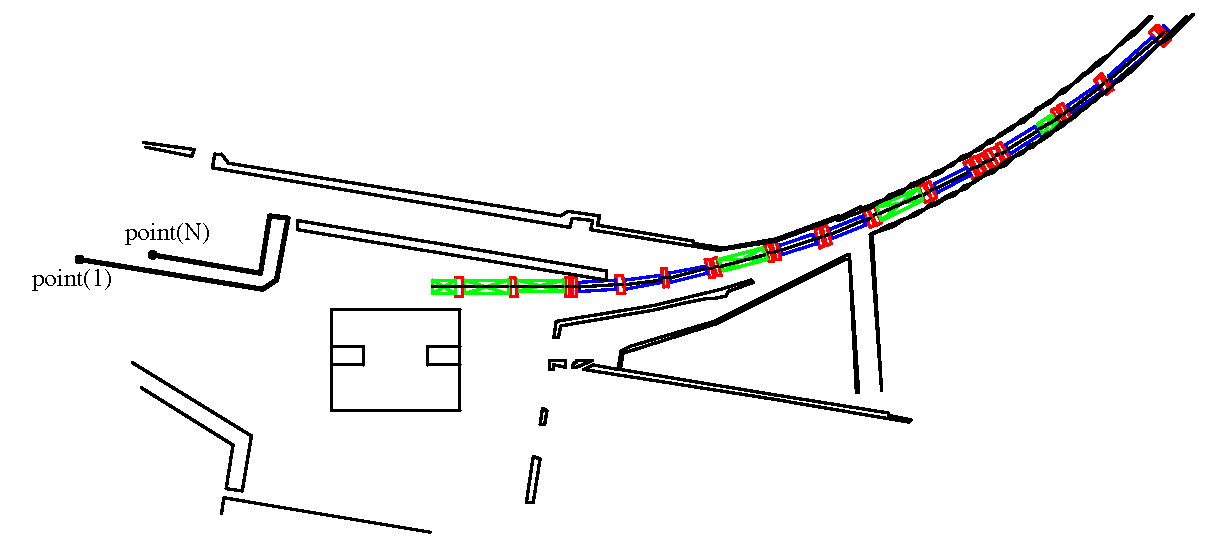
\includegraphics[width=5in]{building-wall.pdf}
  \caption[Floor_plan drawing showing the walls of the building]
{Floor_plan drawing showing the walls of the building (along with a section of a recirculation
arc). Defining building walls can be useful for such things as floor plots and designing a machine
to fit in an existing building.}
  \label{f:building.wall}
\end{figure}

A two dimensional cross-section of the building containing the machine under simulation may be defined in
\tao. This can be useful when drawing \vn{floor_plan} plots of the machine (\sref{s:floor.plan}) or
to design a machine to fit within an existing building by using optimization (\sref{c:opti}).

The wall cross-sections are defined by a set of ``\vn{sections}''. A section is a curve in the
horizontal $Z$-$X$ plane that defines where the face of a wall is. One such section is highlighted in
Figure~\ref{f:building.wall} starting at the point marked ``point(1)'' and ending at the point
marked ``point(N)''. Each section is defined by a set of points which are connected together using
straight lines or circular arcs.

The name of the file containing the building wall definition is given by the \vn{building_wall_file}
variable in the \vn{tao_start} namelist (\sref{s:init.global}). In general, this file will contain a
number of \vn{building_wall_section} namelists. Each \vn{building_wall_section} namelist defines a
single wall section. The syntax of this namelist is
\begin{example}
  &building_wall_section
    \{name = <string>\}
    \{constraint = <type>\}
    point(1) = <z1>, <x1>
    point(2) = <z2>, <x2>, \{<r2>\}
    point(3) = <z3>, <x3>, \{<r3>\}
    ... etc ...
    point(N) = <zN>, <xN>, \{<rN>\}
  /
\end{example}
The optional \vn{name} component allows for matching wall sections to \vn{floor_plan} shapes
(\sref{s:shapes}) when drawing a \vn{floor_plan} so that different portions of the wall can be drawn
in different colors.

The global coordinate system in \bmad (see the \bmad manual) defines the $(Z, X)$ plane as being
horizontal.  [Note: $(Z, X)$ is used instead of $(X, Z)$ since $(Z, X, Y)$ forms a right handed
coordinate system.] The points that define a wall section are specified in this coordinate system.
In the \vn{building_wall_section} namelist, the $(Z, X)$ position of each point defining a wall
section is given along with an optional radius $r$. If a non-zero radius is given for point $j$,
then the segment between point $j-1$ and $j$ is a circular arc of the given radius. If no radius is
given, or if it is zero, the segment is a straight line. A radius for the first point, number 1,
cannot be specified since this does not make sense. Additionally, a radius must be at least half the
distance between the two points that define the end points of the arc.

In general, given two end points and a radius, there are four possible arcs that can be drawn. The
arc chosen follows the following convention:
\begin{enumerate}
\item
The angle subtended by the arc is 180 degrees or less.
\item
If the radius for the arc from $j-1$ to $j$ is positive, the arc curves in a clockwise manner. If
the radius is negative, the arc curves counterclockwise. This convention mimics the convention used
for \vn{rbend} and \vn{sbend} elements.
\end{enumerate}
To define a wall that is circular, use three points with two 180
degree arcs in between.

When designing a machine to fit within the walls of a building, the \vn{constraint} variable of the
namelist is used to designate whether the given wall section is on the $+x$ (left) side of the
machine or the $-x$ (right) side. Here $x$ is the local reference frame transverse coordinate. See
the write up of the \vn{wall.right_side} and \vn{wall.left_side} constraints in \sref{s:data.types}
for more details. Possible values for \vn{constraint} are:
\begin{example}
  "right_side"  ! Section is to be used with wall.right_side constraints
  "left_side"   ! Section is to be used with wall.left_side constraints
  "none"        ! Default. Section is ignored in any constraint calculation.
\end{example}
Using \vn{"none"} for \vn{constraint} is convenient for drawing building components on a
\vn{floor_plan} that are not used as an optimization constraint.

Example:
\begin{example}
  &building_wall_section
    constraint = "left_side"   
    point(1) =  23.2837,    8.2842
    point(2) = -10.9703,   13.8712,   107.345
    point(3) = -10.8229,   14.7737
  /
\end{example}
In this example, point 1 is at $(Z, X) = (23.2837, 8.2842)$, the segment between points 1 and 2 is
an arc with a radius of 107.345 meters, and the segment between points 2 and 3 is a straight
line. Also this wall section is to be used when evaluating any \vn{wall.x+} constraint.

If the machine varies vertically ($y$-direction), vertical constraints may be imposed using the
\vn{floor.y} data type (\sref{s:data.types}).

To see a list of the building wall points when running \tao, use the \vn{show building_wall}
(\sref{s:show.building}) command .

Note: To position a machine in the global coordinate system, the starting point and starting
orientation can be adjusted using \vn{beginning[...]} statements as explained in the \bmad manual.

%-----------------------------------------------------------------
\subsection{Building Orientation}
\label{s:building.orient}

It may be convenient to use a different two-dimensional coordinate system for the horizontal plane
than the global coordinate system used by \bmad and \tao. For example, if the building wall coordinates are
obtained from a blueprint. To help with this, an overall position and angle
shift may be specified by a \vn{building_wall_orientation} namelist in the same file with the
\vn{building_wall_section} namelists. The syntax of the \vn{building_wall_orientation} namelist is:
\begin{example}
  theta = <Real>      ! Angle rotation in radians. Default is 0.
  z_offset = <Real>   ! Z-offset. Default is 0.
  x_offset = <Real>   ! X-offset. Default is 0.
\end{example}
The transformation from the input coordinates of a wall point specified in a \vn{build_wall_section} namelist
to the global coordinate system is
\begin{equation}
  \begin{pmatrix} z \\ x \end{pmatrix}_{global} = 
  \begin{pmatrix} \text{z_offset} \\ \text{x_offset} \end{pmatrix} +
  \begin{pmatrix} \cos(\text{theta}) & -\sin(\text{theta}) \\
                   \sin(\text{theta}) & \cos(\text{theta}) \end{pmatrix} \,
  \begin{pmatrix} z \\ x \end{pmatrix}_{input} 
\end{equation}

%-----------------------------------------------------------------
\section{Dynamic Aperture Calculation Initialization}
\index{dynamic aperture}
\label{s:dynamicaperture}

\begin{figure}
  \centering
  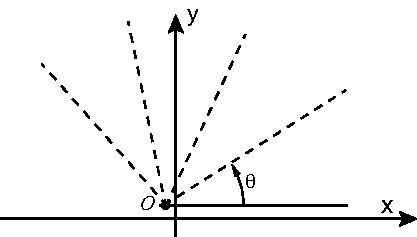
\includegraphics[width=5in]{dynamic-aperture-rays.pdf}
  \caption{
The calculation of a dynamic aperture curve in the $x$-$y$ plane at a given \vn{pz} offset involves
calculating aperture curve points (blue dots) along a set of ``rays'' (dashed lines) having a common
origin point ($\cal O$). The aperture curve is then constructed using linear interpolation between
points. The calculation of an aperture curve point along a given ray involves iteratively tracking
particles with different starting $(x, y)$ position values to find the boundary between stable
(green dots) and unstable (red dots) motion.
  }
  \label{f:da-rays}
\end{figure}

For rings, the dynamic aperture can be calculated and plotted. To calculate the dynamic aperture for
the $i$\Th universe, the \vn{design(i)%dynamic_aperture_calc} parameter must be set True in the
\vn{tao_design_lattice} namelist (\sref{s:init.lat}. Example:
\begin{example}
  &tao_design_lattice
    design_lattice(1)%file = "lat.bmad"
    design_lattice(1)%dynamic_aperture_calc = T
  /
\end{example}
Alternatively, the aperture calculation can be turned on during running using the \vn{set} command
(\sref{s:set.universe}):
\begin{example}
  set universe 1 dynamic_aperture_calc on
\end{example}
Since aperture calculations take time, once an aperture calculation is done, the calculation is
turned off so to perform multiple scans within a given session, the \vn{set universe} command must
be repeatedly done.

The \vn{show dynamic_aperture} command (\sref{s:show.da}) shows parameter values and the
\vn{set dynamic_aperture} command (\sref{s:set.da}) can be used to change parameter values.

If Tao is compiled with the appropriate OpenMP flags, the dynamic aperture calculation will be done
in parallel.

To plot the results, an appropriate plot must be defined (\sref{s:dynamic.ap.plot}) and
\vn{placed} in the plotting window (\sref{s:init.plot}. An example dynamic aperture plot is
shown in Fig.~\ref{f:da-plot}.

Example input files for calculating and plotting the dynamic aperture are at (\sref{s:examples}):
\begin{example}
  \$ACC_ROOT_DIR/tao/examples/dynamic_aperture
\end{example}

Parameters for the dynamic aperture simulation are set in the \vn{tao_dynamic_aperture}
namelist (\sref{s:init.global} in the \tao root initialization file. Example:
\begin{example}
  ! This defines parameters for universe 1.
  &tao_dynamic_aperture
   da_init(1)%ix_branch = 0         ! Lattice branch to use. 0 = default value.
   da_init(1)%pz = 0, 0.01, 0.15    ! List of particle phase space pz.
   da_init(1)%n_angle = 64          ! Number of angles in scan of each energy
   da_init(1)%min_angle = 0         ! Starting scan angle (rad).
   da_init(1)%max_angle = 3.14159   ! Ending scan angle (rad).
   da_init(1)%n_turn = 2000         ! Number of turns a particle must survive
   da_init(1)%x_init = 1e-3         ! initial estimate for horizontal aperture (meters).
   da_init(1)%y_init = 1e-3         ! initial estimate for vertical aperture (meters).
   da_init(1)%accuracy = 1e-5       ! resolution of bracketed aperture (meters)
  /
\end{example}
Dynamic aperture parameters can be defined for each universe. In the above example, parameters are
defined for universe 1. The \vn{pz} parameter array is a list of relative momenta to calculate the
aperture for. One dynamic aperture curve will be produced for each value of \vn{pz}. A dynamic
aperture curve represents the boundary in the $x$-$y$ plane such that if a particle is started with
$p_z$ equal to the given \vn{pz}, and with starting $p_x$, $p_y$, and $z$ set as
described below, then starting the particle with $(x, y)$ coordinates outside of the aperture curve
will result in particle loss and starting the particle with $(x, y)$ coordinates inside the curve
will result in particle survival. Here loss (``unstable motion'') and survival (``stable motion'')
is defined by whether the particle hits an aperture or not over the number of turns set by
\vn{%n_turn} (which is set to 2000 in the above example). The \vn{%ix_branch} parameter sets 
which branch in the lattice is used for tracking.

The calculation of an aperture curve is illustrated in Fig.~\ref{f:da-plot}. To calculate an
aperture curve, a set of ``rays" (dashed lines) having a common origin point ($\cal O$) are
constructed. On each ray, the boundary point between stable and unstable motion (blue points in the
figure) is found by iteratively tracking particles with initial $(x, y)$ points on the ray. The
aperture curve is then constructed using linear interpolation between points. The accuracy with
which the boundary points are calculated is set by the \vn{%accuracy} parameter. The \vn{%x_init}
and \vn{%y_init} values are used as a staring point for the boundary point search. The computed
boundary curve will not depend upon these parameters but having initial values close to the boundary
will same some computation time.

If the RF is off, the origin point of the rays is taken to be the closed orbit at the given
$p_z$. In this case, initial $p_x$ and $p_y$ are set to the closed orbit values, and $z$ is set to
zero (the motion is independent of $z$ so this set does not matter). If the RF is on, the origin
point, along with initial $p_x$, $p_y$, and $z$, are taken equal to the closed orbit (which is not
affected by the initial $p_z$).

The number of rays used is set by the \vn{%n_angle} parameter. In the above example, \vn{n_angle} is
set to 64. The angle of the rays with respect to the $x$-axis ($\theta$ in the figure) will range
from \vn{%min_angle} to \vn{%max_angle}. In the example above the angle ranges from 0 to $pi$.  That
is, the upper half-plane. These are typical settings since typically storage rings are vertically
symmetric so the aperture curves should vertically symmetric as well. The angle between rays is not
uniform but is adjusted to give roughly equally spaced points (this is done by looking at the aperture
points on a horizontal and a vertical ray and then scaling the ray angles appropriately).

%-----------------------------------------------------------------
\section{Initializing Plotting}
\index{plotting initializing}
\label{s:init.plot} 

\subsection{Plot Window}
\label{s:plot.page}
\index{initialization!plotting!plot window}

Plotting is defined by an initialization file whose name is defined by the \vn{plot_file} component
of the \vn{tao_start} namelist (\sref{s:init.global}).  The first namelist block in the file has a
block name of \vn{tao_plot_page}. This block sets the size of the plot window (also called the plot
page) and defines the ``regions'' where plots go. The syntax of this block is:
\index{tao_plot_page}\index{plot_page!n_curve_pts}
\index{plot_page!size}\index{plot_page!border}
\index{plot_page!text_height}\index{plot_page!title}
\index{region!name}\index{region!location}\index{place}
\begin{example}
  &tao_plot_page
    plot_page%plot_display_type        = <string>  ! Display type: "X" or "TK"
    plot_page%size                     = <x_size>, <y_size>         ! size in POINTS 
    plot_page%border                   = <x1\(_{\dstyle{b}}\)>, <x2\(_{\dstyle{b}}\)>, <y1\(_{\dstyle{b}}\)>, <y2\(_{\dstyle{b}}\)>, "<units>"
    plot_page%text_height              = <real>   ! height in POINTS. Def = 12
    plot_page%main_title_text_scale    = <real>   ! Relative to text_height. Def = 1.3
    plot_page%graph_title_text_scale   = <real>   ! Relative to text_height. Def = 1.1
    plot_page%axis_number_text_scale   = <real>   ! Relative to text_height. Def = 0.9
    plot_page%axis_label_text_scale    = <real>   ! Relative to text_height. Def = 1.0
    plot_page%legend_text_scale        = <real>   ! Relative to text_height. Def = 0.8
    plot_page%key_table_text_scale     = <real>   ! Relative to text_height. Def = 0.9
    plot_page%floor_plan_shape_scale   = <real>   ! Floor_plan shape size scaling.
    plot_page%lat_layout_shape_scale   = <real>   ! Lat_layout shape size scaling.
    plot_page%title(i)                 = <string>, {<x>, <y>, "<units>", "<justify>"}
    plot_page%n_curve_pts              = <int>    ! Num points used to construct a 
                                                  !   smooth curve. Default = 401
    plot_page%box_plots                = <T/F>    ! For debugging. Default = F.
    plot_page%delete_overlapping_plots = <T/F>    ! Default = T.
    plot_page%draw_graph_title_suffix  = <T/F>    ! Default = T.
    include_default_plots              = <T/F>    ! Include default templates? Def = T.
    region(i) = "<region_name>" <x1\(_{\dstyle{r}}\)>, <x2\(_{\dstyle{r}}\)>, <y1\(_{\dstyle{r}}\)>, <y2\(_{\dstyle{r}}\)>  
    place(i)  = "<region_name>", "<template_name>"
    default_plot%...                            ! See below.
    default_graph%...                           ! See below. 
  /
\end{example}

%-----------------------

\begin{figure}[bt]
  \centering
  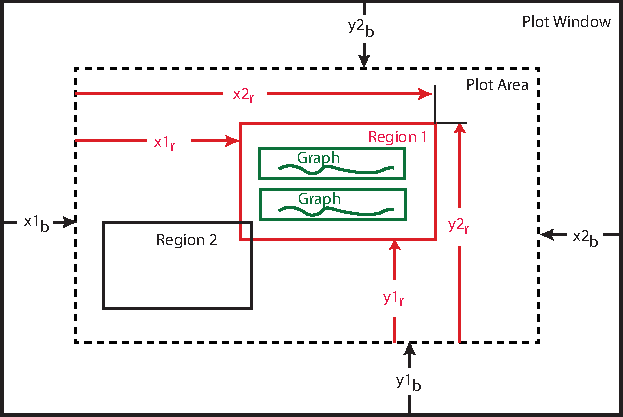
\includegraphics{plot-page.pdf}
  \caption[The plot window.]{The plot window has a boarder whose position is determined by 
the \vn{plot_page\%border} parameter in the tao_plot_page namelist.  Plots are placed
in ``\vn{regions}'' whose location is determined by the setting of the \vn{region(i)} parameters in
the same namelist. Regions may overlap.} 
  \label{f:plot.page}
\end{figure}

%-----------------------

For example:
\begin{example}
  &tao_plot_page
    plot_page%plot_display_type = "X"        ! X11 window.  "TK" is alternative.
    plot_page%size        = 700, 800         ! Points
    plot_page%border      = 0, 0, 0, 50, "POINTS"  
    plot_page%text_height = 12.0
    plot_page%title(1)    = "CESR Lattice", 0.5, 0.996, "%PAGE", "CC"
    region(1) = "top"    0.0, 1.0, 0.5, 1.0
    region(2) = "bottom" 0.0, 1.0, 0.0, 0.5
    place(1)  = "top",    "orbit"
    place(2)  = "bottom", "phase"
    default_plot%x%min = 100
    default_plot%x%max = 200
  /
\end{example}

\vn{plot_page%size} sets the horizontal and vertical size of the plot
window in \vn{points} units (72 points = 1 inch. Roughly 1 point = 1
pixel). 

\vn{plot_page%text_height} sets the overall height of the text that is
drawn. Relative to this, various parameters can be used to scale
individual types of text:
\begin{example}
  plot_page%main_title_text_scale  = 1.3 ! Main title height. 
  plot_page%graph_title_text_scale = 1.1 ! Graph title height.
  plot_page%axis_number_text_scale = 0.9 ! Axis number height
  plot_page%axis_label_text_scale  = 1.0 ! Axis label height.
  plot_page%key_table_text_scale   = 0.8 ! Key Table text (\sref{s:key.table}).
  plot_page%legend_text_scale      = 0.9 ! Lat Layout or floor plan text.
\end{example}
The default values for these scales are given above.

The \vn{plot_page%plot_display_type} component sets the type of plot display
window used. possibilities are:
\begin{example}
  "X"      X11 window
  "TK"     tk window
  "QT"     Available only when using PLPLOT (and not the default PGPLOT)
\end{example}
Note: The environmental variable \vn{ACC_PLOT_DISPLAY_TYPE} sets the default display
type. You can set this variable in your login file to avoid having to setup a \tao
init file to set this.

\vn{plot_page%border} sets a border around the edges of the window. As shown in
Figure~\ref{f:plot.page} x1$_{\dstyle{b}}$, x2$_{\dstyle{b}}$ are the right and left border widths
and y1$_{\dstyle{b}}$ and y2$_{\dstyle{b}}$ are the bottom and top border widths respectively.  The
rectangle within this border is called the plot area.

\vn{plot_page%title(i)} set the page title. There are two title areas (i = 1,2). If only the title
string is given then the other variables are set to the defaults \vn{x} = 0.5, \vn{y} = 0.995,
\vn{justify} = "CC" and \vn{units} = "\vn{%PAGE}". See the QuickPlot documentation
(\sref{s:line.symb}) for more details.

The plot area is divided up into rectangular regions where plots may be placed (what defines a plot
is discussed below).  \vn{region(i)} in the \vn{tao_plot_page} namelist is an array of five elements
that defines the i\Th region. The first element of this array is the name of the region. This name
may not contain a dot ``.''.  The last four elements of the \vn{retion(i)} array, x1$_{\dstyle{r}}$,
x2$_{\dstyle{r}}$, y1$_{\dstyle{r}}$ and y2$_{\dstyle{r}}$ define the location of the region as
illustrated in Figure~\ref{f:plot.page}.  x1$_{\dstyle{r}}$ and x2$_{\dstyle{r}}$ are normalized to
the width of the plot area and y1$_{\dstyle{r}}$ and y2$_{\dstyle{r}}$ are normalized to the height
of the plot area. That is, these four number should be in the range $[0, 1]$.  Regions may overlap
any one can define as many regions as one likes.

Besides the regions that the user sets up in the \vn{tao_plot_page} namelist, \tao defines a number
of default regions whose names begin with the letter ``\vn{r}''. Use the \vn{show plot} command
(\sref{s:plot}) to view a list of these plots.

When \vn{plot_page%delete_overlapping_plots} is True (the default), Placing a plot (using
the \vn{place} command \sref{s:place}) causes any existing plots that overlap the
placed plot to become invisible. 

The \vn{plot_page%draw_graph_title_suffix} is used to suppress the drawing of the string that
is printed to the right of a graph title (set by \vn{graph%title}). This string is set by \tao
and has information on what is being plotted (typically the \vn{curve%component}). To suppress
the suffix, set \vn{plot_page%draw_graph_title_suffix} to False.

The \vn{plot_page%n_curve_pts} parameter sets the default number of points to use for drawing
``smooth'' curves. The default is 401. This default may be overridden for individual plots by
setting the \vn{plot%n_curve_pts} component of a plot (\sref{s:template}). If \vn{plot%n_curve_pts}
is set for an individual plot, that value overrides the value of
\vn{plot_page%n_curve_pts}. Warning: \tao will cache intermediate calculations used to compute a
smooth curve to use in the computation of other smooth curves. \tao will only do this for curves
that have \vn{plot_page%n_curve_pts} number of points. Depending upon the circumstances, setting
\vn{plot%n_curve_pts} for individual plots may slow down plotting calculations significantly.

The \vn{place(i)} commands, $i = 1,2,3,\ldots$ determine the initial placement of plots. The initial
placement can be modified while \tao is running using the \vn{place} command (\sref{s:place}).

\vn{default_plot} sets the defaults for any \vn{plot}s defined in the \vn{tao_template_plot}
namelists (\sref{s:template}). Similarly, \vn{default_graph} sets defaults for the \vn{graph}
structure defined in the \vn{tao_template_graph} namelist (\sref{s:template}). In the example above,
the default x-axis min and max are set to 100 and 200 respectively.

If \vn{include_default_plots} is set to \vn{False}, the collection of default template
plots (\sref{s:template}) that \tao uses by default are not used along with the template
plots defined in the plotting file.

%-----------------------------------------------------------------
\subsection{Plot Templates}
\label{s:template}
\index{plot templates}

As shown in Figure~\ref{f:plot}, a ``plot'' is made up of a collection of ``graphs'' and a graph
consists of axes plus a set of ``curves''. To define custom plots, there needs to be defined
a set of ``template plots''. A template plot specifies the layout of a plot: How the graphs are
placed within a plot, what curves are associated with what graphs, etc. When running \tao, the
information in a template plot may then be transferred to a region using the \vn{place} command and
this will produce a visible plot.

The file that \tao looks in to find plotting information is set by the \vn{plot_file} component of
the \vn{tao_start} namelist (\sref{s:init.global}). The default, if \vn{plot_file} is not set, is
the root initialization file.

Template plots are defined using namelists with a name of \vn{tao_template_graph}. The general
syntax is:
\index{tao_template_plot}
\index{plot!name}
\index{plot!x}
\index{plot!x_axis_type}
\index{plot!n_graph}
\index{plot!autoscale_gang_x}
\index{plot!autoscale_gang_y}
\index{plot!autoscale_x}
\index{plot!autoscale_y}
\begin{example}
  &tao_template_plot
    plot%name        = "<plot_name>"
    plot%x           = <qp_axis_struct>
    plot%x_axis_type = "<x_axis_type>"   ! "index", "ele_index" "s", "lat", "var", etc. 
    plot%n_graph     = <n_graphs>
    plot%autoscale_gang_x = <logical>    ! Default: True.
    plot%autoscale_gang_y = <logical>    ! Default: True.
    plot%autoscale_x = <logical>         ! Default: False.
    plot%autoscale_y = <logical>         ! Default: False.
    plot%n_curve_pts = <integer>         ! Used to override plot_page%n_curve_pts.
    default_graph%...                    ! See below
  /
\end{example}
For example:
\begin{example}
  &tao_template_plot
    plot%name                = "orbit"
    plot%x%min               =   0
    plot%x%max               = 100
    plot%x%major_div_nominal = 10
    plot%x%label             = "Index"
    plot%n_graph             = 2
    default_graph%y%max      = 10
  /
\end{example}

\vn{default_graph} sets defaults for the \vn{graph} structure defined in the \vn{tao_template_graph}
namelist (\sref{s:template}). This overrides \vn{default_graph} settings made in the
\vn{tao_template_plot} namelist (\sref{s:init.plot}) but only for graphs associated with the
\vn{tao_template_plot} the \vn{default_graph} is defined in.

\vn{plot%x} sets the properties of the horizontal axis. For more information see the \vn{QuickPlot}
documentation (\sref{s:line.symb}) on the \vn{qp_axis_struct}.  If \vn{min} and \vn{max} are absent,
then \tao will autoscale the axis.  If it is desired to have differing scales for different graphs,
the \vn{graph%x} component can be used (see below).

Both \vn{major_div} and \vn{major_div_nominal} set the number of major divisions in the plot. The
difference between the two is that with \vn{major_div} the number of major divisions is fixed at the
set value and with \vn{major_div_nominal} the number of major divisions can vary from the set value
when \tao scales a graph. If \vn{major_div_nominal} is set, this will override any setting of
\vn{major_div}. If neither \vn{major_div} nor \vn{major_div_nominal} is set, a value will be chosen
for \vn{major_div_nominal} by \tao. If you are unsure which to set, it is recommended that
\vn{major_div_nominal} be used.

Plots with \vn{plot%autoscale_x} and/or \vn{plot%autoscale_y} logicals, set to true will
automatically rescale after any calculation. The \vn{plot%autoscale_gang_x} and
\vn{plot%autoscale_gang_y} components set how the \vn{x_scale} (\sref{s:x.scale}) and \vn{scale}
(\sref{s:scale}) commands behave when autoscaling entire plots. See these individual commands for
more details.

The \vn{plot%n_plot_pts} parameter sets the number of points to use for drawing ``smooth''
curves. This overrides the setting of \vn{plot_page%n_plot_pts} (\sref{s:init.plot}). Warning: \tao
will cache intermediate calculations used to compute a smooth curve to use in the computation of
other smooth curves. \tao will only do this for curves that have \vn{plot_page%n_curve_pts} number
of points. Depending upon the circumstances, setting \vn{plot%n_curve_pts} for individual plots may
slow down plotting calculations significantly.

\vn{plot%name} is the name that is used with \tao commands to identify the plot. It is important
that this name not contain any blank spaces since \tao uses this fact in parsing the command line.

\vn{plot%x_axis_type} sets what is plotted along the
\vn{x_axis}. Possibilities are:
\index{index}
\index{ele_index}
\index{s}
\begin{example}
    "index"         ! Data Index.
    "ele_index"     ! Element lattice number index.
    "s"             ! Longitudinal position in the lattice.
    "s_expression"  ! s-dependent expression involving lattice parameters.
    "data"          ! From a data array.
    "lat"           ! Lattice variable. See \sref{s:plot.var}.
    "var"           ! Tao variable value. See \sref{s:plot.var}.
    "phase_space"   ! Set by \tao if graph%type = "phase_space".
    "none"          ! Set by \tao if graph%type = "key_table".
    "floor"         ! Set by \tao if graph%type = "floor_plan".
\end{example}

The \vn{ele_index} switch is used when plotting data arrays. In this
case the \vn{index} switch refers to the index of the data array and
\vn{ele_index} refers to the index of the lattice element that the
datum was evaluated at.

\vn{n_graph} sets the number of graphs associated with the plot and
each one needs a \vn{tao_template_graph} namelist to define it. These
namelists should be placed directly after their respective
\vn{tao_template_graph} namelists. The general format of the
\vn{tao_template_graph} namelist is:
\index{tao_template_graph}\index{graph!y}\index{curve!name}
\index{graph_index}\index{graph}\index{graph!name}\index{curve}
\index{graph!type}\index{graph!box}\index{graph!title}\index{graph!margin}
\index{graph!y2}\index{graph!n_curve}\index{graph!clip}\index{graph!component}
\index{graph!symbol_size_scale}
\index{curve!data_type}\index{curve!data_source}
\index{curve!x_axis_units_factor}\index{curve!y_axis_units_factor}
\index{curve!use_y2}\index{curve!line}\index{curve!ele_ref_name}
\index{curve!draw_line}\index{curve!draw_symbols}\index{curve!ix_universe}
\index{curve!symbol}\index{curve!symbol_every}\index{curve!convert}
\index{curve!ix_bunch}\index{curve!data_type_x}
\begin{example}
  &tao_template_graph
    graph_index             = <integer>
    graph%name              = "<string>"       ! Default is  "g<n>" <n> = graph_index. 
    graph%type              = "<string>"       ! "data", "floor_plan", etc.
    graph%box               = <ix>, <iy>, <ix_tot>, <iy_tot>
    graph%title             = "<string>"       ! Title above the graph.
    graph%title_suffix                         ! Not user settable.
    graph%margin            =  <ix1>, <ix2>, <iy1>, <iy2>, "<Units>"
    graph%scale_margin      =  <ix1>, <ix2>, <iy1>, <iy2>, "<Units>"
    graph%x                 = <qp_axis_struct> ! Horizontal axis.
    graph%y                 = <qp_axis_struct> ! Left axis.
    graph%x2                = <qp_axis_struct> ! Top axis (only used for floor_plan plots).
    graph%y2                = <qp_axis_struct> ! Right axis.
    graph%y2_mirrors_y      = <logical>        ! y2 min/max the same as y-axis? Default = T
    graph%clip              = <logical>        ! Clip curves at boundary? Default = T
    graph%draw_axes         = <logical>        ! Default = T
    graph%draw_grid         = <logical>        ! Default = T
    graph%allow_wrap_around = <logical>        ! Wrap curves around lattice ends?
    graph%component         = "<string>"       ! Eg: "model - design"
    graph%symbol_size_scale = <real>                  ! Phase_space plots symbol scale factor
    graph%ix_universe       = <integer>               ! Default = -1 => Use default universe
    graph%floor_plan        =  <floor_plan_struct>    ! Floor_plan parameters (\sref{s:floor.plan}).
    graph%draw_only_good_user_data_or_vars     ! Veto data or variables with good_user = F?
                                 = <logical>   !   Default = T.
    graph%x_axis_scale_factor    = <factor>    ! Scale the x-axis by this.
    graph%n_curve                = <integer>   ! number of curves
    curve(i)%name                = "<string>"  ! Default is "c<i>", <i> = curve num.
    curve(i)%data_source         = "<string>"  ! Source for the data curve points
    curve(i)%data_type_x         = "<string>"  ! Used with plot%x_axis_type = "data" or "var".
    curve(i)%data_type           = "<string>"  ! EG: "orbit.x"
    curve(i)%component           = "<string>"  ! Eg: "model - design". Overrides graph%component.
    curve(i)%data_index          = "<string>"  ! Index number for data points.
    curve(i)%legend_text         = "<string>"  ! Text for curve legend. 
                                               !   Default is the data_type.
    curve(i)%y_axis_scale_factor = <factor>    ! Scale the y-axis by this.
    curve(i)%use_y2              = <logical>   ! Use left-axis scale?
    curve(i)%draw_line           = <logical>   ! Connect data with lines?
    curve(i)%draw_symbols        = <logical>   ! Draw data symbols?
    curve(i)%draw_symbol_index   = <logical>   ! Print index number next to the data symbol?
    curve(i)%draw_error_bars     = <logical>   ! Draw error bars with data?
    curve(i)%ix_universe         = <integer>   ! Default = -1 => Use graph%ix_universe.
    curve(i)%ix_branch           = <integer>   ! Default = 0  => Use main lattice.  
    curve(i)%ix_bunch            = <integer>   ! Bunch index. Default = 0 (all bunches).
    curve(i)%line        = <qp_line_struct>    ! Line spec (color, width, etc.)
    curve(i)%symbol      = <qp_symbol_struct>  ! Symbol spec (color size, etc.)
    curve(i)%symbol_every     = <integer>      ! Plot symbol every # datums
    curve(i)%ele_ref_name     = "<string>"     ! Name of reference element.
    curve(i)%smooth_line_calc = <Logical>      ! Calc data between symbol points? 
    curve(i)%units            = "<string>"     ! Data units
  /
\end{example}
For example:
\begin{example}
  &tao_template_graph
    graph_index               = 1
    graph%name                = "x"
    graph%type                = "data"
    graph%box                 = 1, 1, 1, 2
    graph%title               = "Horizontal Orbit (mm)"
    graph%margin              =  60, 200, 30, 30, "POINTS"
    graph%y%label             = "X"
    graph%y%max               =  4
    graph%y%min               = -4
    graph%y%major_div_nominal = 4
    graph%n_curve             = 1
    graph%component           = "model - design"
    curve(1)%data_source      = "data"
    curve(1)%data_type        = "orbit.x"
    curve(1)%units_factor     = 1000
    curve(1)%use_y2           = F
  /
\end{example}
See the QuickPlot documentation (\sref{s:line.symb}) description of the \vn{qp_symbol_struct} and the
\vn{qp_line_struct}.

\vn{graph%title} is the string just above the graph. The full string will also include information
about what is being plotted and the horizontal axis type. To fully suppress the title leave it
blank. Note: A graph also has a \vn{graph%title_suffix} which \tao uses to hold the string which is
printed to the right of the \vn{graph%title}. This string contains information like what
\vn{curve%component} is being plotted. The \vn{graph%title_suffix} cannot be set by the user.

If there are multiple curves drawn with a graph then a curve legend showing what lines are
associated with what data will be drawn. The default is to draw this legend in the upper left hand
corner of the graph. By default, the \vn{data_type} of each curve will be used as the text for that
curve's line in the legend.  This default can be changed by setting a curve's \vn{curve%legend_tex}.

\vn{graph%name} and \vn{curve%name} define names to be used with commands. The default names are
just the letter \vn{g} or \vn{c} with the index of the graph or curve. Thus, in the example above,
the name of the curve defaults to \vn{c1} and it would be referred to as \vn{orbit.x.c1}.  It is
important that these names do not contain any blank spaces since \tao uses this fact in parsing the
command line.

\vn{graph%box} sets the layout of the box which the \vn{graph} is placed in. For a definition of
what a box is see the QuickPlot documentation (\sref{s:line.symb}). In the above example the graph
divides the region into two vertically stacked boxes and places itself into the bottom one.

\vn{graph%allow_wrap_around} sets if, for a lattice with closed geometry, the curves contained in
the graph are ``wrapped'' around the end of the lattice if \vn{graph%x%min} is negative. The default
is \vn{True}. This only applies if \vn{plot%x_axis_type} is set to \vn{"s"}.

\vn{graph%margin} sets the margin between the \vn{graph} and the \vn{box}
it is drawn in.

\vn{graph%scale_margin} is used to set the minimum space between what is being drawn and the edges
of the \vn{graph} when a \vn{scale}, \vn{x_scale}, or a \vn{xy_scale} command is issued. Normally
this is zero but is useful for \vn{floor plan} drawings.

\vn{graph%type} is the type of graph. \tao knows about the
following types:
\index{data}\index{lat_layout}\index{key_table}\index{phase_space}
\index{floor_plan}\index{beam_chamber_wall}
\begin{example}
  "data"               ! Lattice parameters, data and/or variable plots (default) (\sref{s:plot.data}).
  "dynamic_aperture"   ! Dynamic aperture plot (\sref{s:dynamic.ap.plot}
  "floor_plan"         ! A 2-dimensional birds-eye view of the machine (\sref{s:floor.plan}).
  "histogram"          ! Histogram of plot (\sref{s:histogram}).
  "key_table"          ! Key binding table for single mode (\sref{s:key.table}).
  "lat_layout"         ! Schematic showing placement of the lattice elements (\sref{s:lat.layout}).
  "phase_space"        ! Phase space plots (\sref{s:phase.space}).
\end{example}

With \vn{graph%type} set to \vn{"beam_chamber_wall"} (\sref{s:beam.wall.draw}), the beam chamber
wall is drawn if it has been defined in the \bmad lattice file.

With \vn{graph%type} set to \vn{"data"} (\sref{s:plot.data}), data such as orbits and/or variable
values such as quadrupole strengths are plotted. Here ``data'' can be data from a defined data
structure (\sref{c:data}) or computed directly from the lattice, beam tracking, etc. A \vn{"data"}
graph type will contain a number of \vn{curves} and multiple data and variable curves can be drawn
in one graph.

With \vn{graph%type} set to \vn{floor_plan} (\sref{s:floor.plan}), the two dimensional layout of the
machine is drawn.

With \vn{graph%type} set to \vn{histogram} (\sref{s:histogram}), such things such as beam densities
can be histogrammed.

With \vn{graph%type} set to \vn{"key_table"} (\sref{s:key.table}), the key bindings for use in
single mode (\sref{s:key.bind}) are displayed.  Note: The \vn{"key_table"} graph type does not have
any associated \vn{curve}s.

With \vn{graph%type} set to \vn{lat_layout} (\sref{s:lat.layout}), the elements of the lattice are
symbolical drawn in a one dimensional line as a function of the longitudinal distance along the
machine centerline.

With \vn{graph%type} set to \vn{phase_space} (\sref{s:phase.space}), phase space plots are produced.

%-----------------------------------------------------------------
\subsection{Lattice Parameters, Data and Variable plotting}
\label{s:plot.data}

A \vn{graph} (\sref{s:template}), with \vn{graph%type} equal to \vn{"data"}, is used to draw lattice
parameters such as orbits, or \tao data (\sref{c:data}), or variable values such as quadrupole
strengths. A data \vn{graph} will have a number of associated \vn{curve}s with each curve defining a
particular data type to plot.

The data values will depend upon where the data comes from. This is determined, in part, by the
setting of \vn{graph%component} and \vn{curve%component}. \vn{graph%component} and
\vn{curve%component} may be one of:
\index{model}\index{design}\index{base}\index{meas}\index{ref}
\begin{example}
  "model"             ! model values. Default.
  "design"            ! design values.
  "base"              ! Base values
  "meas"              ! data values.
  "ref"               ! reference data values.
  "beam_chamber_wall" ! Beam chamber wall
\end{example}
Additionally, \vn{graph%component} may be set to plot a linear combination of the above. For
example:
\begin{example}
  graph%component = "model - design"
\end{example}
This will plot the difference between the \vn{model} and \vn{design} values.

If \vn{curve%component} is set, it will override \vn{graph%component}. If \vn{graph%component} is
not set in the initialization file, and if there are curves of the graph that have not been set,
\vn{graph%component} will be given a default setting of \vn{model}.

\index{data}\index{var}\index{calculation}
\index{curve!data_source}
The \vn{curve} structure is used to define the data that is plotted in each graph.
\vn{curve%data_source} is the type of information for the source of the data points.
\vn{curve%data_source} must be one of:
\begin{example}
  "data"              ! A d1_data array is the source of the curve points.
  "var"               ! A v1_var array is the source of the curve points.
  "lat" (Default)     ! The curve points are computed directly from the lattice.
  "beam"              ! The curve points are computed tracking a beam of particles.
  "multi_turn_orbit"  ! Computation is from multi-turn tracking. 
\end{example}
The default for \vn{curve%data_source} is \vn{"lat"}. With \vn{curve%data_source} set to \vn{data},
the values of the curve points come from the \vn{d1_data} array structure named by
\vn{curve%data_type}. Thus in the above example the curve point values are obtained from
\vn{orbit.x} data. To be valid the data structure named by \vn{curve%data_type} must be set up in an
initialization file. If not given, the default \vn{curve%data_type} is
\begin{example}
  <plot%name>.<graph%name>
\end{example}
If \vn{curve%data_source} is set to \vn{var}, the values of the curve points come from a \vn{v1_var}
array structure. If it is set to \vn{lat} the curve data points are calculated from the lattice
without regard to any data structures. \vn{curve%data_source} can be set to \vn{beam} when tracking
beams of particles. In this case, the curve points are calculated from the tracking. With \vn{beam},
the particular bunch that the data is extracted from can be specified via \vn{curve%ix_bunch}. The
default is \vn{0} which combines all the bunches of the beam for the calculation.

Example: With \vn{curve%data_type} set to \vn{beta.x}, the setting of \vn{curve%data_source} to
\vn{lat} gives the beta as calculated from the lattice and \vn{beam} gives the beta as calculated
from the shape of the beam.

\vn{curve%draw_symbols} determines whether a symbol is drawn at the data points. The size, shape and
color of the symbols is determined by \vn{curve%symbol}. A given symbol point that is drawn has
three numbers attached to it: The $(x, y)$ position on the graph and an index number to help
identify it. The index number of a particular symbol is the index of the datum or variable
corresponding the symbol in the \vn{d1_data} or \vn{v1_var} array. These three numbers can be
printed using the \vn{show curve -symbol} command (\sref{s:show}).  \vn{curve%draw_symbol_index}
determines whether the index number is printed besides the symbol. Use the \vn{set curve} command
(\sref{s:set}) to toggle the drawing of symbols. The default value for \vn{curve%draw_symbol} is
False if \vn{plot%x_axis_type} is \vn{"s"}, \vn{"curve"}, \vn{"lat"}, or \vn{"var"} and True
otherwise. The default \vn{curve%draw_symbol_index} is always False.

\vn{curve%draw_line} determines whether a curve is drawn through the data point symbols. The
thickness, style (solid, dashed, etc.), and color of the line can be controlled by setting
\vn{curve%line}. If \vn{plot%x_axis_type} is \vn{"s"}, and \vn{graph%component} does not contain
\vn{"meas"} or \vn{"ref"}, \tao will attempt to calculate intermediate values in order to draw a
smooth, accurate curve is drawn. Occasionally, this process is too slow or not desired for other
reasons so setting \vn{curve%smooth_line_calc} to False will prevent this calculation and the curve
will be drawn as a series of lines connecting the symbols. The default of
\vn{curve%smooth_line_calc} is True. Use the \vn{set curve} command (\sref{s:set}) to toggle the
drawing of lines. Alternatively, the \vn{-disable_smooth_line_calc} switch can be used on the
command line (\sref{s:command.line}) or the global variable \vn{global%disable_smooth_line_calc} can
be set in the \tao initialization file (\sref{s:globals}).

The \vn{graph%draw_only_good_user_data_or_vars} logical determines whether datums
(\sref{s:init.data}) or variables (\sref{s:init.var}) with a \vn{good_user} component set to
\vn{False} are drawn. The default is to not draw them which means that data or variables not used in
an optimization are not drawn.

A graph has two vertical axes. The one on the left is called \vn{"y"} and the one on the right is
called \vn{"y2"}. For example, \vn{graph%y%label} sets the axis label for the \vn{y} axis and
\vn{graph%y2%label} sets the axis label for the \vn{y2} axis. Normally there is only one vertical
scale for a graph and this is associated with the \vn{y} axis. However, if any curve of a given
graph has \vn{curve%use_y2} set to \vn{True} then the \vn{y2} axis will have an independent second
scale. In this case, the \vn{y2} axis numbers will be drawn. Notice that simply giving the \vn{y2}
axis a label does {\em not} make the \vn{y2} axis scale independent of the \vn{y} axis scale.

Typically, a graph's horizontal scale is set by the \vn{plot%x} component. If it is desired to have
differing scales for different graphs, the \vn{graph%x} component can be used.

The \vn{curve%draw_error_bars} logical determines whether error bars are drawn when plotting data
(\vn{curve%data_source} set to \vn{data}). The half height of the error bars is determined by the
\vn{error_rms} values of the data associated with the curve (\sref{s:data.anatomy}).  To keep things
simple, \tao ignores the setting of \vn{curve%component} when drawing error bars. This must be kept
in mind since for example, the measurement error associated with a difference plot of measured data
- reference data (when \vn{curve%component} is set to \vn{meas-ref}) is different from just plotting
measured data, which in turn is different from a plot of the data as calculated from the \vn{model}
(the measurement error associated with this is zero).

The \vn{curve%ele_ref_name} component is only used if \vn{curve%data_source} is set to \vn{"lat"}.
If \vn{curve%ele_ref_name} is set, the curve will be shifted by subtracting the value of the
parameter being plotted evaluated at the reference element. For example, if \vn{orbit.x} is being
plotted, and \vn{curve%ele_ref_name} is set to "\vn{Q10W}", the plotted curve will be shifted by
subtracting the value of the horizontal orbit at Q10W. Notice that the shifting is done for each
graph component. For example, if \vn{graph%component} is set to "\vn{model - design}", the curve
will be shifted by subtracting the difference between the \vn{model} and \vn{design} values
evaluated at the reference element.

%-----------------------------------------------------------------
\subsection{Graphing a Data Slice}\index{plot!data slice}
\label{s:graph.data.slice}

Note: Data slicing is a type of parametric plotting. For parametric plotting using curve data see
section~\sref{s:param.plot}.

The standard data graph, as presented in the previous subsection, plots data from a given
\vn{d1_data} array. It is also possible to graph data that has been ``sliced'' in other ways. For
example, suppose a number of universes have been established, with each universe representing the
same machine but with different steerings powered. If in each universe an \vn{orbit} \vn{d2_data}
structure has been defined, an example of a data slice is the collection of points (x, y) where:
\begin{example}
  (x, y) = (<n>@orbit.x[23], <n>@orbit.y[23]),   <n> = 1, ..., n_universe
\end{example}
When defining a template for graphing a data slice, the plot%x_axis_type is set to \vn{"data"}, and
the \vn{graph%type} must be set to \vn{"data"}, the \vn{curve(:)%data_source} must be set to
\vn{"data"} and the \vn{curve(:)%data_type_x} and \vn{curve%data_type} are used to define the x and
y axes respectively.  In the strings given by \vn{<curve%data_type_x} or \vn{<curve%data_type}, all
substrings that look like \vn{\#ref} are eliminated and the string given by \vn{curve%ele_ref_name}
is substituted in its place.  Similarly, a \vn{\#comp} string is used as a place holder for the
\vn{graph%component} Example:
\begin{example}
  &tao_template_plot
    plot%name = "at_bpm"
    plot%x%label = "x"
    plot%x_axis_type = "data"
    plot%n_graph = 1
  /

  &tao_template_graph
    graph_index = 1
    graph%title = "Orbit at BPM"
    graph%y%label = "y"
    graph%component = "meas - ref"
    graph%type = "data"
    graph%n_curve = 1
    graph%x_axis_scale_factor = 1000
    curve(1)%data_source = "data"
    curve(1)%data_type_x = "[2:57]@orbit.x[#ref]|#comp"
    curve(1)%data_type   = "[2:57]@orbit.y[#ref]|#comp"
    curve(1)%data_index  = "[2:57]@orbit.y[#ref]|ix_uni"
    curve(1)%y_axis_scale_factor = 1000
    curve(1)%ele_ref_name = "23"
    curve(1)%draw_line = F
  /
\end{example}
In this example, \vn{curve(1)%data_type_x} expands to \vn{"[2:57]@orbit.x[23]|meas-ref"}. That is,
the \vn{meas - ref} values of \vn{orbit.x[23]} from universes 2 through 57 is used for the x-axis.
Similarly, \vn{orbit.y[23]} is used for the y-axis. The \vn{set} command (\sref{s:set}) can be used
to change \vn{curve%ele_ref_name} and \vn{graph%component} strings.

\vn{curve%data_index} sets the index number for the symbol points (\sref{s:template}). In the above
example, \vn{curve%data_index} is set to \vn{"[2:57]@orbit.y[\#ref]|ix_uni"}. The \vn{|ix_uni}
component will result in the symbol index number being the universe number.  Additionally, the
component \vn{|ix_d1} can be used to specify the index in the \vn{d1_data} array, and the component
\vn{|ix_ele} can be used to specify the lattice element index. Setting the symbol index number is
important when \vn{curve%draw_symbol_index} is set to True so that the symbol index is drawn with
the curve. Additionally, the command \vn{show curve -symbol} (\sref{s:show}) will print the symbol
index number along with the $(x, y)$ coordinates of the symbols.

Arithmetic expressions (\sref{s:arithmetic.exp}) may be mixed with explicit datum components in the
specification of \vn{curve(:)%data_type_x} and \vn{curve(:)%data_type}. Example:
\begin{example}
  curve(1)%data_type_x = "[#ref]@orbit.x|model"
  curve(1)%data_type   = "[#ref]@orbit.x|meas-ref"
  curve(1)%ele_ref_name = "3"
\end{example}
The plots the \vn{model} values of \vn{orbit.x} verses \vn{meas - ref} of \vn{orbit.x} for the data
in universe 3. Note: Whenever explicit components are specified, the \vn{graph%component} settings
are ignored for that expression.

%-----------------------------------------------------------------
\subsection{Plotting With a Variable Parameter on the X-Axis}
\index{plot!plotting as a function of a variable}
\label{s:plot.var}

Data can be plotted as a function of a lattice parameter by setting \vn{plot%x_axis_type} to
\vn{"lat"} (for lattice variables) or \vn{"var"} (for \tao variables) and setting
\vn{curve(:)%data_type_x} to the name of the variable. In this case, the \vn{curve(:)%data_type}
must evaluate to a single number.

Example:
\begin{example}
  &tao_template_plot
    plot%x_axis_type = "lat"
    plot%n_curve_pts = 50
    ...
  /

  &tao_template_graph
    ...
    curve(1)%data_type_x = "particle_start[x]"  ! X-axis values.
    curve(1)%data_type   = "orbit.x[10]"        ! Y-axis values.
    ...
  /
\end{example}
Here the number of curve points has been set to 50 to reduce the evaluation overhead.

Note: \tao treats the \vn{design} and \vn{base} lattices as static so that varying a variable will
not affect these lattices. Thus, constructing a plot with \vn{graph%component} set to, for example,
\vn{"model - design"} will {\em not} produce a plot that is the difference between varying a
variable in both \vn{model} and \vn{design} lattices. In the case where such a plot is desired, a
second universe needs to be established. In this case, one would set \vn{curve(:)%data_type} to
something like
\begin{example}
    curve(1)%data_type   = "1@orbit.x[10] - 2@orbit.x[10]"    
\end{example}
where the universe \#2 \vn{model} lattice would be setup to be equal to the universe \#1 \vn{design}
lattice.

%-----------------------------------------------------------------
\subsection{Drawing a Lattice Layout}
\index{lattice layout}
\label{s:lat.layout}

\begin{figure}
  \centering
  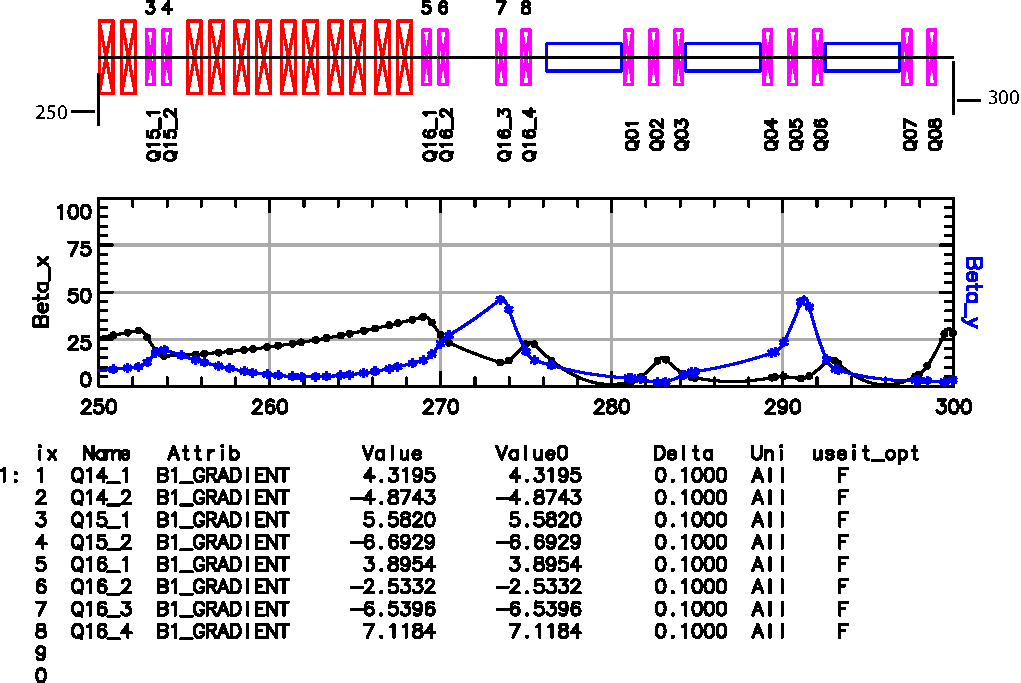
\includegraphics[width=5in]{layout-graph-table.pdf}
  \caption[Example lattice layout and data plots]
{A lattice layout plot (top) above a data plot (middle) which in turn is above a key table plot
(bottom). The points on the curves in the data plot mark the edges of the elements displayed in the
lattice layout. Elements that have attributes that are varied as shown in the key table have the
corresponding key table number printed above the element's glyph in the lattice layout.}
  \label{f:layout.table}
\end{figure}

A lattice layout plot draws the lattice along a straight line with colored rectangles representing
the various elements.  An example is shown in Figure~\ref{f:layout.table}.  The
\vn{tao_template_plot} needed to define a lattice layout looks like:
\index{tao_template_plot}\index{plot!name}
\index{plot!x!min}\index{plot!x!max}\index{plot!n_graph}
\index{tao_template_graph}\index{graph_index}\index{graph!name}
\index{graph!type}\index{graph!title}\index{graph!box}
\index{graph!ix_universe}\index{graph!margin}\index{graph!n_curve}
\begin{example}
  &tao_template_plot
    plot%name        = "<plot_name>"
    plot%x%min       = <real>  
    plot%x%max       = <real>  
    plot%n_graph     = <integer>
    plot%x_axis_type = "s"
  /
  &tao_template_graph
    graph_index       = <integer>
    graph%name        = <name>
    graph%type        = "lat_layout"
    graph%title       = "Layout Title"
    plot%box          = <ix>, <iy>, <ix_tot>, <iy_tot>
    graph%ix_universe = <integer> ! -1 => use current default universe
    graph%ix_branch   = <integer> !  0 => use main lattice.
    graph%margin      = <ix1>, <ix2>, <iy1>, <iy2>, "<Units>"
    graph%y%min       = <real>    ! Default: -100
    graph%y%max       = <real>    ! Default:  100
  /
\end{example}
Example:
\begin{example}
  &tao_template_plot
    plot%name        = "layout"
    plot%x%min       =   0
    plot%x%max       = 100
    plot%n_graph     = 1
    plot%x_axis_type = "s"
  /

  &tao_template_graph
    graph_index       = 1
    graph%name        = "u1"
    graph%type        = "lat_layout"
    graph%box         = 1, 1, 1, 1
    graph%ix_universe = -1  ! Use default universe
    graph%margin      = 0.12, 0.12, 0.30, 0.06, "%BOX"
  /
\end{example}

Which elements are drawn is under user control and is defined using an \vn{lat_layout_drawing}
namelist. See Section~\sref{s:shapes} for more details.

Setting \vn{graph%ix_universe} to -1 means the current default universe will be drawn. Normally, if
there are element shapes that are associated with data or variable shapes (\sref{s:shapes}), these
shapes will be drawn if there are lattice elements associated with the data or variables that live
in the universe with index \vn{graph%ix_universe} and if the associated elements fall within the
range of elements plotted. The exception is that if \vn{graph%ix_universe} is set to -2, the universe
of the associated lattice elements is ignored. Using a value of -2 here only makes sense if the design
lattices of all the universes is the same.

The longitudinal distance markers at either end of the lattice layout can be suppressed by setting
\begin{example}
  graph%x%draw_numbers = F
\end{example}

%-----------------------------------------------------------------
\subsection{Drawing a Floor Plan}
\index{floor plan drawing}
\label{s:floor.plan}

\begin{figure}[b]
  \centering
  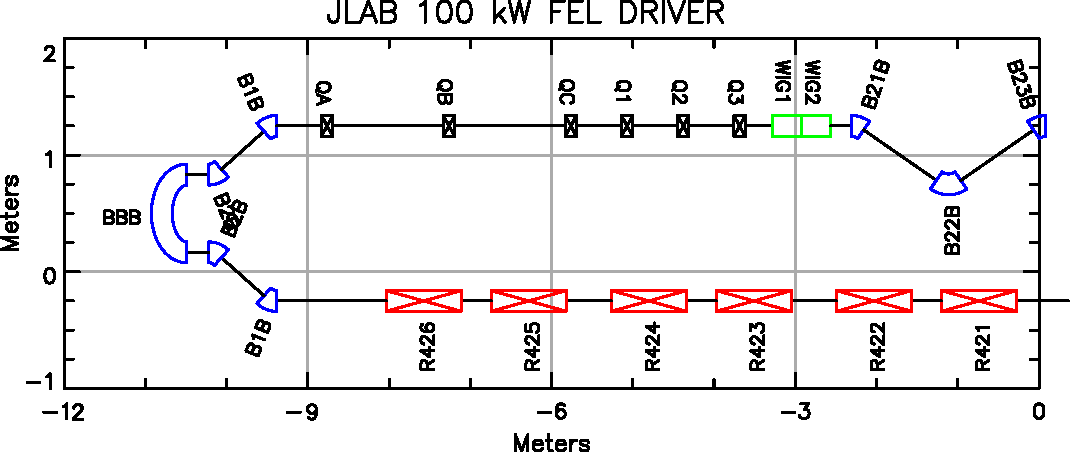
\includegraphics[width=5in]{floor-plan.pdf}
  \caption{Example Floor Plan drawing.}
  \label{f:floor.plan}
\end{figure}

A \vn{floor plan} drawing gives a display of the machine projected onto the horizontal plane.  An
example is shown in Figure~\ref{f:floor.plan}. Like a \vn{Lattice Layout} (\sref{s:lat.layout}),
Elements are represented by colored rectangles and which elements are drawn is determined by a
\vn{floor_plan_drawing} namelist (see~\sref{s:shapes}). Additionally, a cross-section of the walls
of the building containing the machine (\sref{s:building.wall}) can be drawn along with the
reference orbit (which is the closed orbit for machines with a closed geometry). This is illustrated
in Figure~\ref{f:floor.orbit}.

The placement of a lattice element in the drawing is determined by the element's coordinates in the
\vn{global reference system}.  See the Bmad manual for more information on the \vn{global reference
system}.  In the \vn{global reference system}, the $(Z, X)$ plane is the horizontal plane. 

A floor plan orbit is associated with a \vn{graph} of a \vn{plot} (\sref{s:template}). A \vn{graph}
has a \vn{floor_plan} component which is a structure of type \vn{tao_floor_plan_struct}. Components
of this structure can be set to control how a floor plan is drawn. The components of a
\vn{tao_floor_plan_struct} are:
\begin{example}
  type tao_floor_plan_struct
    rotation             = <real>      ! Rotation of floor plan plot: 1.0 -> 360 deg. 
    view                 = "<string>"  ! View plane for floor plan plot. default = "zx"
    correct_distortion   = <logical>   ! For Floor Plan plots: Default = F
    flip_label_side      = <logical>   ! Draw element label on other side of element?
    size_is_absolute     = <logical>   ! Shape sizes scaled to absolute dimensions?
    draw_only_first_pass = <logical>   ! Draw only first pass with multipass elements?
    orbit_scale          = <real>      ! Scale for the orbit. Default = 0 => No orbit drawn.
    orbit_color          = "<color>"   ! Line color. Default = "red".
    orbit_pattern        = "<pattern>" ! Line pattern. Default = "solid_line".
    orbit_width          = <integer>   ! Line width. Default = 1.
  end type
\end{example}
A graph is initialized with a \vn{tao_template_graph} namelist (\sref{s:template}). Example:
\begin{example}
  &tao_template_graph
    ...
    graph%floor_plan%rotation = 0.5  ! Rotate 180 degrees
    graph%floor_plan%orbit_scale = 100
    graph%floor_plan%orbit_color = "red"
    graph%floor_plan%orbit_width = 3
  /
\end{example}

The \vn{scale} component scales the displacement of the orbit from the lattice reference coordinate
system (which is the centerline of the lattice elements if there are no misalignments). So a value
of 100.0, a 1~cm orbit is drawn 1~meter from the centerline. A setting of zero (the default) means
that the orbit is now drawn. Note: If \vn{scale} is not unity, the plotted orbit when going through
a \vn{patch} element with a finite transverse offset will show a discontinuity due to the
discontinuity of the reference orbit.

What plane a floor plan is projected onto is determined by the setting of the
\vn{graph%floor_plan%view} switch. This switch is a two character string.  Each character is either
"x", "y", or "z" and the characters must not be both the same. Default is "zx". The first character
determines which global coordinate is mapped to the horizontal axis of the graph and the second
character determines which global coordinate is mapped to the vertical axis of the graph. There are
six possible two character combinations. The default "zx" setting represents looking at the
horizontal plane from above. A setting of "xz" represents looking at the horizontal plane from
below. The other combinations involving "y" are only potentially useful if the machine has a significant
vertical extent.

%----------------
\begin{figure}[b]
  \centering
  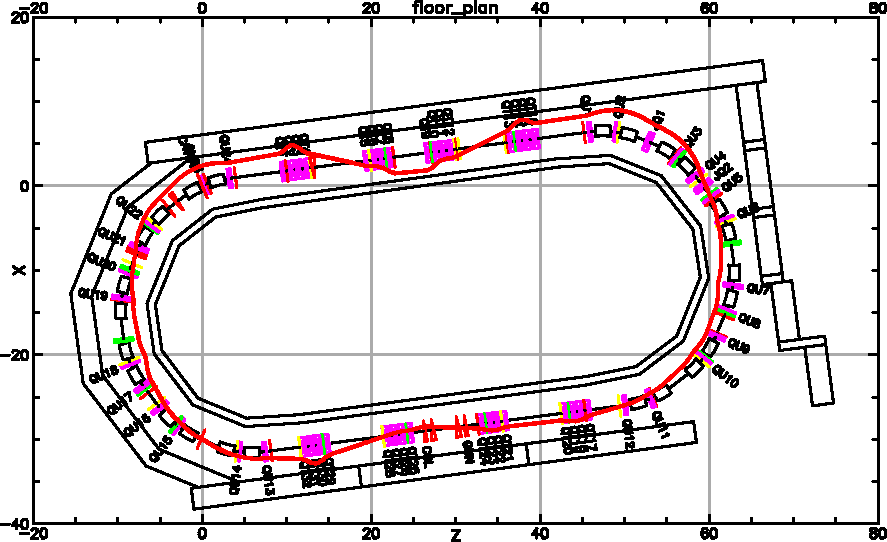
\includegraphics[width=5in]{floor-plan-orbit.pdf}
  \caption[Floor plan with orbit and building walls.]{Example Floor plan drawing with the closed orbit 
(red line) and building walls included.}
  \label{f:floor.orbit}
\end{figure}
%----------------

If element labels are to be drawn, on which side the labels are drawn can be flipped by setting 
\vn{graph%floor_plan%flip_label_side} to True.

The \vn{size_is_absolute} logical is combined with the \vn{<size>} setting for a shape to determine the
size transverse to the center line curve of the drawn shape (\sref{s:shapes}).
If \vn{size_is_absolute} is False (the default), \vn{<size>} is taken to be the size of
the shape in points (72 points is approximately 1 inch). If \vn{size_is_absolute} is True,
\vn{<size>} is taken to be the size in meters. That is, if \vn{size_is_absolute} is
False, zooming in or out will not affect the size of an element shape while if
\vn{size_is_absolute} is True, the size of an element will scale when zooming.

An overall rotation of the floor plan can be controlled by setting \vn{rotation} parameter. A
setting of 1.0 corresponds to 360$^\circ$. Positive values correspond to counter-clockwise
rotations.  Alternatively, the global coordinates at the start of the lattice can be defined in the
lattice file and this can rotate the floor plan.  Unless there is an offset specified in the lattice
file, a lattice will start at $(x, y) = (0, 0)$. Assuming that the machine lies in the horizontal
plane with no negative bends, the reference orbit will start out pointing in the negative $x$
direction and will circle clockwise in the $(x, y)$ plane.

The \vn{draw_only_first_pass} logical, if set True, suppresses drawing of \vn{multipass_slave}
lattice elements that are associated with the second and higher passes. This logical defaults to
False. Setting to True is only useful in some extreme circumstances where the plotting of additional
passes leads to large pdf/ps file sizes.

Note: If \vn{graph%ix_universe} is set to -1 the current viewed universe is used. If
\vn{graph%ix_universe} is set to -2, all universes are plotted.

Example Floor Plan template:
\begin{example}
  &tao_template_plot
    plot%name = "floor"
    plot%x%min = -12  
    plot%x%max = 0    
    plot%x%major_div_nominal = 4
    plot%x%minor_div = 3
    plot%n_graph = 1
  /

  &tao_template_graph
    graph_index = 1
    graph%name = "1"
    graph%type = "floor_plan"
    graph%box = 1, 1, 1, 1
    graph%margin = 0.10, 0.10, 0.10, 0.10, "%BOX"
    graph%ix_universe = -2   ! Draw all universes.
    graph%x%label = "SMART LABEL"
    graph%y%label = "SMART LABEL"
    graph%y%max = 2  
    graph%y%min = -1 
    graph%floor_plan%correct__distortion = T
    graph%floor_plan%size_is_absolute = T
    graph%floor_plan%view = "xz"  ! Looking from beneath
    graph%floor_plan%orbit_scale = 100
  /
\end{example}

Having \vn{graph%x%label} and \vn{graph%y%label} set to ``\vn{SMART LABEL}'' means that the actual axis labels will be 
picked appropriately based upon the setting of \vn{graph%floor_plan%view}.

To prevent the drawing of the axes set \vn{graph%draw_axes} to False.  To prevent the drawing of a
grid at the major division points set \vn{graph%draw_grid} to False.

By default, the horizontal or vertical margins of the graph will be increased so that the horizontal
scale (meters per plotting inch) is equal to the vertical scale.  If
\vn{graph%floor_plan%correct_distortion} is set to \vn{False}, this scaling will not be done.

Note: The \vn{show ele -floor} command (\sref{s:show}) can be used to view an element's global
coordinates.

%-----------------------------------------------------------------
\subsection{Defining Shapes for Lat_layout and Floor_plan Drawings}
\label{s:shapes}
\index{lat_layout drawings}
\index{floor_plan drawings}

\vn{Floor plan} (\sref{s:floor.plan}) and \vn{lattice layout} drawings use various shapes, sizes,
and colors to represent lattice elements. The association of a particular element with a given shape
is determined via two namelists: \vn{lat_layout_drawing} for the lattice layout and
\vn{floor_plan_drawing} for floor plan drawings.  Two different namelists are used since, for
example, a size that is good for a layout will not necessarily be good for a floor plan.

The file that \tao looks in to find these two namelists is set by the first file specified in the
\vn{plot_file} array set in the \vn{tao_start} namelist (\sref{s:init.global}). The default, if
\vn{plot_file} is not set, is the root initialization file.

The namelist syntax is the same for both:
\begin{example}
  &lat_layout_drawing
    include_default_shapes = <logical>
    ele_shape(i) = "<ele_id>" "<shape>" "<color>" "<size>" "<label>" <draw> 
                                                                <multi> <line_width>
  /

  &floor_plan_drawing
    ... same as lat_layout_drawing ...
  /
\end{example}
For Example:
\begin{example}
  &floor_plan_drawing
    include_default_shapes = T
    !               ele_id                  Shape        Color     Size  Label  ..etc..
    ele_shape(1) = "quadrupole::q*"         "box"        "red"     0.75  "name"  
    ele_shape(2) = "quadrupole::*"          "xbox"       "red"     0.75  "none" 
    ele_shape(3) = "sbend::sb*"             "box"        "blue"    0.37  "none"
    ele_shape(4) = "sbend::*"               "box"        "blue"    0.37  "none"  
    ele_shape(5) = "wiggler::*"             "xbox"       "green"   0.50  "name"
    ele_shape(6) = "var::quad_k1"           "circle"     "purple"  0.25  "name"
    ele_shape(7) = "data::orbit.x|design"   "vvar:box"   "orange"  0.25  "name"
    ele_shape(8) = "building_wall::*"       "solid_line" "black"    0    "none"
    ele_shape(3)%multi = T
    ele_shape(5:6)%line_width = 5, 6
  /
\end{example}
A figure is drawn for each lattice element in the lattice that matches the \vn{<ele_id>} field
(\sref{s:ele.list.format}). Thus, in the example above, \vn{ele_shape(1)} will match to all
quadrupoles whose name begins with ``q'' and \vn{ele_shape(2)} will match all quadrupoles.

Besides the usual element class prefixes (\vn{quadrupole::}, \vn{sbend::}, etc.), other prefixes
that can be used with an \vn{<ele_id>} are
\begin{example}
  data::            ! Match to \tao datum name.
  var::             ! Match to \tao variable name.
  alias::           ! Match to lattice element alias parameter.
  type::            ! Match to lattice element type parameter.
  building_wall::   ! Used in floor_plan plots.
\end{example}
The \vn{data::} prefix is used to match to data that will be used in an optimization. Thus, in the
above example, \vn{ele_shape(7)} specifies that an ``x'' will be drawn at points where there is
valid \vn{orbit.x} data. For this to work, an \vn{orbit.x} data array must be defined
(\sref{s:init.data}).

The \vn{var::} prefix is used for drawing variable locations for variables used in an
optimization. In the above example, it is assumed that a \vn{quad_k1} variable array has been
setup. A circle will be drawn at each element under control of a \vn{quad_k1} variable.

For \vn{floor_plan} drawings, the building wall (\sref{s:building.wall}) can be drawn by specifying
an \vn{ele_shape} whose name is \vn{"building_wall::<name>"} where \vn{<name>} is used to match to
the building wall section name. Use ``\vn{*}'' for \vn{<name>} to match to all names. For the
building wall, the only attribute that is relevant is the \vn{<color>} attribute.

The \vn{alias::} and \vn{type::} prefixes for \vn{<ele_id>} are used to match to the \vn{alias} and
\vn{type} string parameters of that can be set in the lattice file for each individual element.

If an element matches more than one shape,
what is drawn depends upon the setting of \vn{<multi>}. If \vn{<multi>} is False (the default) for
the first shape matched in the list of shapes, only this shape will be used.  If \vn{<multi>} is
True, \tao will draw this shape and then look for additional matches. Each time an additional match
is found, the shape is drawn and the setting of \vn{<multi>} for that shape will be used to
determine whether additional shapes are searched for. Thus \vn{<multi>} can be use to draw, for
example, a \vn{circle} shape superimposed upon a \vn{bow_tie} shape.

\tao defines a set of default shapes in case no shapes are defined in the plot file. If the
optional \vn{include_default_shapes} logical, which can be set for either \vn{floor_plan} and/or
\vn{lat_layout} shape namelists, is set to False (the default), the default shapes are not used.
If \vn{include_default_shapes} is set to True, the default shapes are appended to the list of 
shapes.

Use the \vn{show plot -floor_plan} and \vn{show plot -lat_layout} commands to see the defined
shapes. Use the \vn{set floor_plan} and \vn{set lat_layout} commands (\sref{s:set})) to set shape
parameters on the command line.

The width of a drawn shape is the width of the associated element. The exception is the \vn{"x"}
shape whose width is always the same as the height determined by the \vn{<size>} setting.

\vn{<size>} is the half height of the shape. That is, the size transverse to the longitudinal
dimension. For \vn{lat_layout} drawings, \vn{<size>} = 1.0 corresponds to full scale if the default
\vn{graph%y%min} = -1 and \vn{graph%y%max} = 1 are used. For {floor_plan} drawings, the drawn size
is also affected by the setting of \vn{graph%floor_plan%size_is_absolute} See \sref{s:floor.plan}
for more details.

The overall size of all the shapes can be scaled using the \vn{plot_page} (\sref{s:init.plot})
parameters
\begin{example}
  floor_plan_shape_scale     ! For floor_plan drawings. Default = 1
  lat_layout_shape_scale     ! For lat_layout drawings. Default = 1
\end{example}

The text size in both \vn{floor_plan} and \vn{lat_layout}
plots can be scaled by using the \vn{plot_page} parameter
\begin{example}
  legend_text_scale          ! Default = 1
\end{example}
Use the \vn{show plot} command to view these parameters. Use the
\vn{set plot_page} command to set these parameters.

\vn{<color>} is the color of the shape. Good colors to use are:
\index{element shape!color}
\begin{example}
  "black"
  "blue"
  "cyan"
  "green"
  "magenta"
  "orange"
  "purple"
  "red"
  "yellow"
\end{example}

The \vn{<line_width>} parameter is an integer that specifies the width of the lines drawn. The
default is 1.

The \vn{<label>} indicates what type of label to print next to the corresponding
element glyph. Possibilities are:
\begin{example}
  name            -- The element name (default).
  none            -- No label is drawn.
  s               -- Draw longitudinal s position.
\end{example}
The default is \vn{"name"}

The \vn{<draw>} field determines if a shape is drawn or not. The default is \vn{T}. This can be
useful for toggling on and off the drawing of shapes using the \vn{set shape} command
(\sref{s:set}).

Note: There is an old, deprecated syntax where both the lattice layout and floor plan drawings are
specified via one \vn{element_shapes} namelist.

The \vn{<shape>} parameter is the shape of the figure drawn. The \vn{<shape>} string will have the
form:
\begin{example}
  <shape-name>  or
  <prefix>:<shape-name>  
\end{example}
Valid \vn{shape-name}s are: 
\index{box}\index{xbox}
\begin{example}
  "box"            -- Rectangular box
  "bow_tie"        -- Bow-tie shape.
  "circle"         -- Circle centered at center of element.
  "diamond"        -- Diamond shape.
  <pattern_name>   -- Custom shape specified by <name>. Used with "pattern" prefix.
  "rbow_tie"       -- Bow-tie shape rotated 90 degrees.
  "d_triangle"     -- Triangle pointing ``down''.
  "l_triangle"     -- Triangle pointing ``left'' (upstream).
  "r_triangle"     -- Triangle pointing ``right'' (downstream).
  "u_triangle"     -- Triangle pointing ``up''. 
  "x"              -- "X" centered at center of element
  "xbox"           -- Rectangular box with an x through it.
  "dashed_line"    -- Only used with ele_id set to "building_wall".
  "dash_dot_line"  -- Only used with ele_id set to "building_wall".
  "dotted_line"    -- Only used with ele_id set to "building_wall".
  "solid_line"     -- Only used with ele_id set to "building_wall".
\end{example}
Valid prefixes are:
\begin{example}
  "asym_var"   -- Like "var" prefix but is not symmetric about the center line.
  "asym_vvar"  -- Like asym_var except scaled to associated variable or datum.
  "pattern"    -- Custom shape. <shape-name> here is a pattern name.
  "var"        -- Shape with variable height. 
                       The shape size is symmetric about the center line.
  "vvar"       -- Like "var" prefix except scaled to associated variable or datum.
\end{example}

For example, if an element's shape is set to \vn{var:box} or \vn{asym_var:box}, the drawn size of the
element is proportional to the element's magnetic or electric strength. The associated
\vn{<size>} setting is the multiplier used to scale from element strength to height. For
example, for a quadrupole the height is proportional to the \vn{K1} focusing strength. The
difference between \vn{var:box} or \vn{asym_var:box} is that with \vn{var:box} the drawn
box is symmetric with respect to the centerline with a size independent of the sign of the
element strength. On the other hand, with \vn{asym_var:box}, the drawn box will terminate
with one side on the centerline and the side on which it is drawn will depend upon the the
sign of the element strength. Note: Not all lattice elements can be used with a
\vn{var:box} or \vn{asym_var:box}.

A \vn{vvar:box} shape is like a \vn{var:box} and a \vn{asym_vvar:box} is like a
\vn{asym_var:box}. The difference is that \vn{vvar:box} and \vn{asym_vvar:box} shapes may only be
used when the \vn{<ele_id>} is associated with data or variables. That is, when the \vn{<ele_id>}
string starts with ``\vn{data::}'' or ``\vn{var::}''. In this case, the height of the box, instead
of being proportional to the strength of the element, is proportional to the value of the associated
datum or variable. If no datum or variable component is specified in the \vn{ele_id}, the model
value will be used. Thus, in the above example, where \vn{<ele_id>} was set to
\vn{"data::orbit.x|design"}, the design value is used.

The \vn{solid_line}, \vn{dashed_line}, \vn{dash_dot_line}, and \vn{solid_line} settings for
\vn{<shape>} is used when \vn{<ele_id>} is set to \vn{building_wall} to indicate what type of line
is to be drawn.

The \vn{pattern:<pattern_name>} shape allows for a custom pattern to be specified. Custom
patterns are specified by a \vn{shape_pattern} namelist:
\begin{example}
  &shape_pattern
    name = "<curve_name>"
    line%width = <line_width>
    pt(1) = <s>, <x>
    pt(2) = <s>, <x>
    pt(3) = ...
  /
\end{example}
Example:
\begin{example}
  &floor_plan_drawing
    ...
    ele_shape(2) = "quadrupole::*"     "pattern:q_pat"     "red"     0.75     "none" 
    ...
  /

  &shape_pattern
    name = "q_pat"
    pt(1) = 0, -1
    pt(2) = 1, -1
    pt(3) = 0.9, 1
    pt(4) = 0.1, 1
    pt(5) = 0, -1
  /
\end{example}
The \vn{name} of the \vn{shape_pattern} namelist (in this example it is "q_pat") must match the name
given by \vn{"pattern:<pattern_name>"}. The pattern is specified by a number of points. Between the
points, a line segment is drawn. In the above example, the pattern is an isosceles trapezoid.  When
drawn, the \vn{s} coordinate is scaled so that $s = 0$ corresponds to the entrance end of the
element and $s = 1$ corresponds to the exit end. The \vn{x} coordinate is scaled by the \vn{size}
attribute of the \vn{ele_shape}. The color of the line segments is set by the definition and the width
of the line segments is set by the pattern definition.

%-----------------------------------------------------------------
\subsection{Drawing Apertures}
\index{aperture drawing}
\label{s:draw.ap}

\begin{figure}
  \centering
  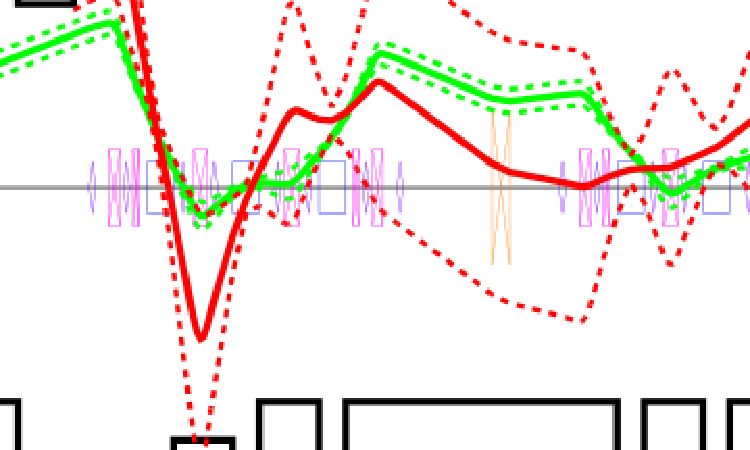
\includegraphics[width=6in]{aperture-plot.pdf}
  \caption[Example beam aperture plot.]
{Example plot of the beam aperture. In this drawing, two turns of three injected particles are drawn. The
particles start at different positions and illustrate what the size of an injected beam would be. Also drawn
(a bit faint) is a \vn{lat_layout} showing lattice element positions.}
  \label{f:aperture}
\end{figure}

Beam apertures can be defined in the \bmad lattice file. Apertures can be defined in one of three
ways. The most common is to set limit or aperture parameters for an element. Another possibility 
is to use a \vn{mask} element (which can be used to define an aperture of arbitrary shape). The
third possibility involves defining a continuous three-dimensional wall. This third possibility 
is only used with Runge-Kutta type tracking. 

To simplify things, the drawing of the beam aperture ignores any \vn{mask} elements (since the
geometry can be very complicated here) and ignores any three-dimensional walls (which are only
used for Runge-Kutta type tracking). \fig{f:aperture} shows an example of a aperture drawing.

To draw an aperture, a curve's \vn{data_source} parameter must be set to \vn{"aperture"} and the \vn{data_type} parameter is set to one of
\begin{example}
  "+x"     ! Aperture in +X direction
  "-x"     ! Aperture in -X direction
  "+y"     ! Aperture in +Y direction
  "-y"     ! Aperture in -Y direction
\end{example}
The apertures in the $+x$ and $+y$ directions will have positive values and the apertures in the
$-x$ and $-y$ directions will have negative values. Set the curve's \vn{y_axis_scale_factor} to scale
tye aperture curve if needed.

The following example will graphs the horizontal orbit along with the horizontal apertures.
\begin{example}
  &tao_template_plot
    plot%name        = "x_orbit"
    plot%x_axis_type = "s"
    plot%n_graph     = 1
  /

  &tao_template_graph
    graph%name    = "x"
    graph_index   = 1
    graph%n_curve = 3

    curve(1)%data_source  = "aperture"
    curve(1)%data_type    = "+x"
    curve(1)%draw_symbols = T
    curve(1)%draw_line    = F
    curve(1)%data_source  = "aperture"
    curve(2)%data_type    = "-x"
    curve(2)%draw_symbols = T
    curve(2)%draw_line    = F
    curve(3)%data_type = "orbit.x"
  /
\end{example}
Note: Aperture curves will ignore the \vn{curve%component} parameter.

%-----------------------------------------------------------------
\subsection{Drawing Dynamic Aperture Curves}
\index{dynamic aperture drawing}
\label{s:dynamic.ap.plot}

A \vn{dynamic_aperture} drawing displays the results of the dynamic aperture
calculation (\sref{s:dynamicaperture}). Example plot setup:
\begin{example}
&tao_template_plot
  plot%name = "da"
  plot%x%min = -20
  plot%x%max =  20
  plot%x%major_div_nominal = 10
  plot%x%label = "x (mm)"
  plot%x_axis_type = "phase_space"
  plot%n_graph = 1
/

&tao_template_graph
  graph%name = "g1"
  graph%type = "dynamic_aperture"
  graph_index = 1
  graph%title = "dynamic aperture"
  graph%margin =  0.15, 0.06, 0.12, 0.12, "%BOX"
  graph%x_axis_scale_factor = 1000
  graph%y%label = "y (mm)"
  graph%y%label_offset = .2
  graph%y%major_div = 4
  graph%n_curve = 3
  curve(1:3)%y_axis_scale_factor = 3*1000
  curve(1:3)%draw_symbols = 3*F
  curve(3)%data_type = "physical_aperture"
  curve(3)%line%color = "red"
  curve(3)%line%width = 5 
/
\end{example}
This produces Fig.~\ref{f:da-plot}.  Each curve represents a single momentum
calculation.  If there are more momenta than curves (as in this case), additional curves will
automatically be created using the styles of the previous curves. Note that apertures are calculated
at element 0.

\begin{figure}
  \centering
  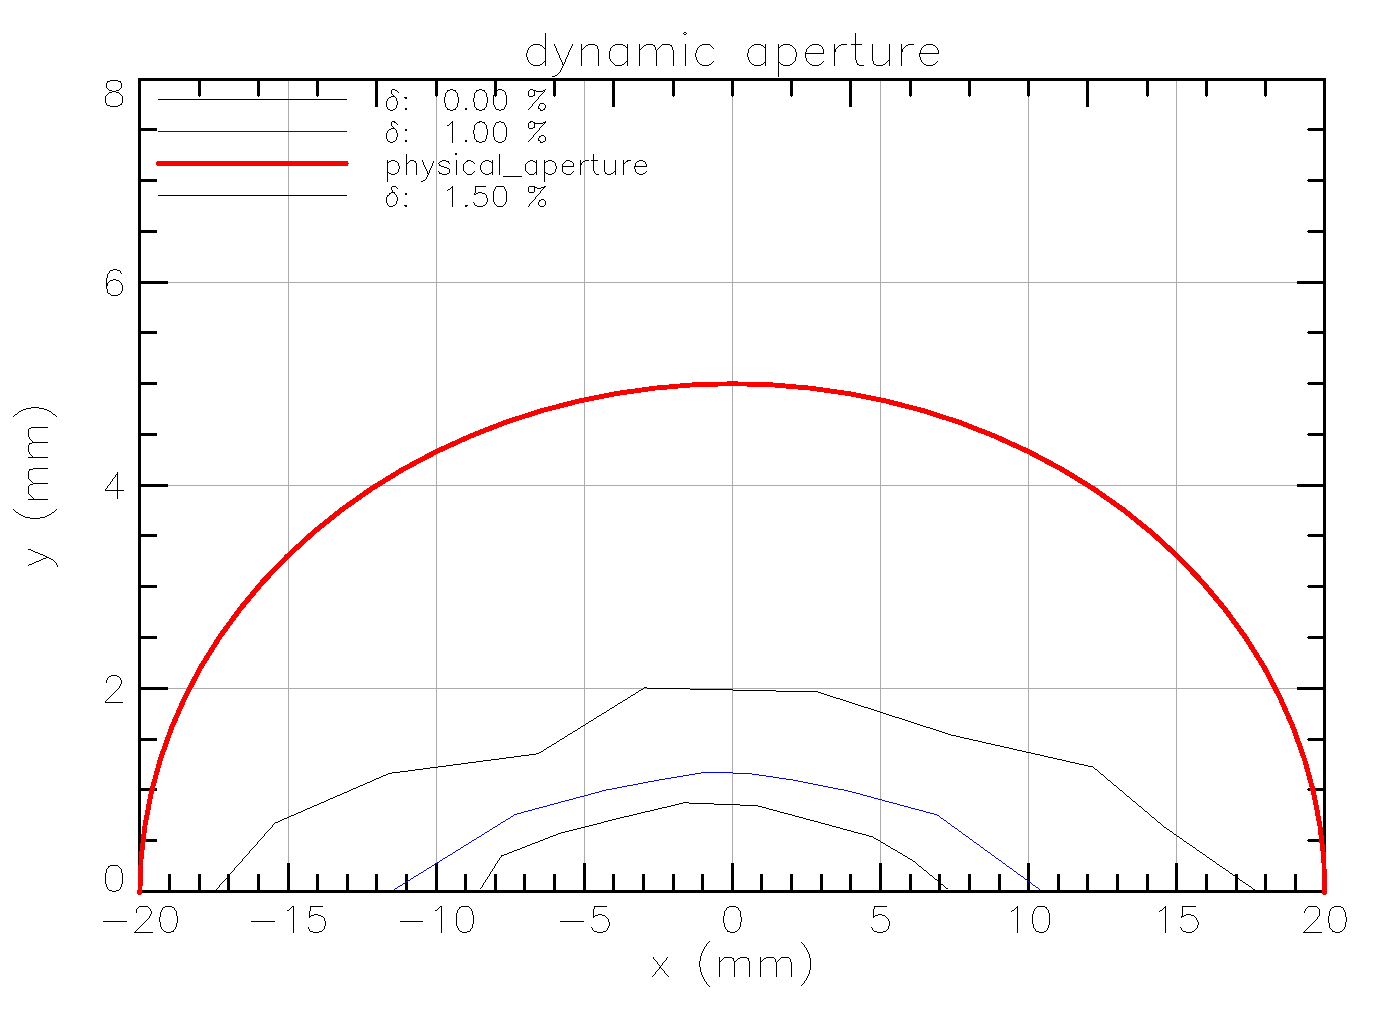
\includegraphics[width=5in]{dynamic-aperture.pdf}
  \caption{Example dynamic aperture plot.}
  \label{f:da-plot}
\end{figure}

If there is a curve with \vn{%data_type} set to \vn{"physical_aperture"}, and if there is a lattice
element at $s = 0$ that has an aperture set, this physical aperture will be drawn. Example: In the
\bmad lattice file define a marker element with an aperture and superimpose the marker at the
beginning of the lattice:
\begin{example}
  m: marker, x_limit = 0.045, y_limit = 0.025, superimpose
\end{example}

Dynamic aperture curves can have the following \vn{%data_type}:
\begin{example}
  "dynamic_aperture" or ""    ! (default) points include the reference orbit
  "dynamic_aperture_centered" ! points are centered (relative to) the reference orbit
  "physical_aperture"         ! draws the physical aperture based on x1_limit, etc. 
\end{example}

%-----------------------------------------------------------------
\subsection{Drawing a Histogram}
\index{histogram drawing}
\label{s:histogram}

A \vn{histogram} drawing displays a histogram of phase space beam density. Histogram plotting is
associated with a \vn{graph} by setting \vn{graph%type} equal to \vn{"histogram"}. The concepts here
are similar to \vn{phase space} plotting (\sref{s:phase.space}). An example is shown in
Fig.~\ref{f:histogram}, using the example histogram template:
\begin{example}
&tao_template_plot
  plot%name = "zhist"
  plot%x%min = -6
  plot%x%max =  6
  plot%x%label = "z (mm)"
  plot%n_graph = 1
/

&tao_template_graph
  graph_index = 1
  graph%name = "z"
  graph%type = "histogram"
  graph%box = 1, 1, 1, 1
  graph%title = "Bunch Histogram: Z"
  graph%margin =  0.15, 0.06, 0.12, 0.12, "%BOX"
  graph%y%label = "Current (A)"
  graph%n_curve = 1
  graph%y%label_offset = .1
  graph%x_axis_scale_factor = 1000.00 !m->mm

  curve(1)%hist%density_normalized = T
  curve(1)%hist%weight_by_charge = T
  curve(1)%hist%number = 100
  curve(1)%line%color = "blue"
  curve(1)%line%pattern = "dashed"
  curve(1)%y_axis_scale_factor = 299792458  !Q/m * c_light
  curve(1)%data_type = "z" 
  curve(1)%data_source = "beam_tracking"
  curve(1)%ele_ref_name = "BEGINNING"
  curve(1)%symbol%type = "dot"
/
\end{example}

\begin{figure}
  \centering
  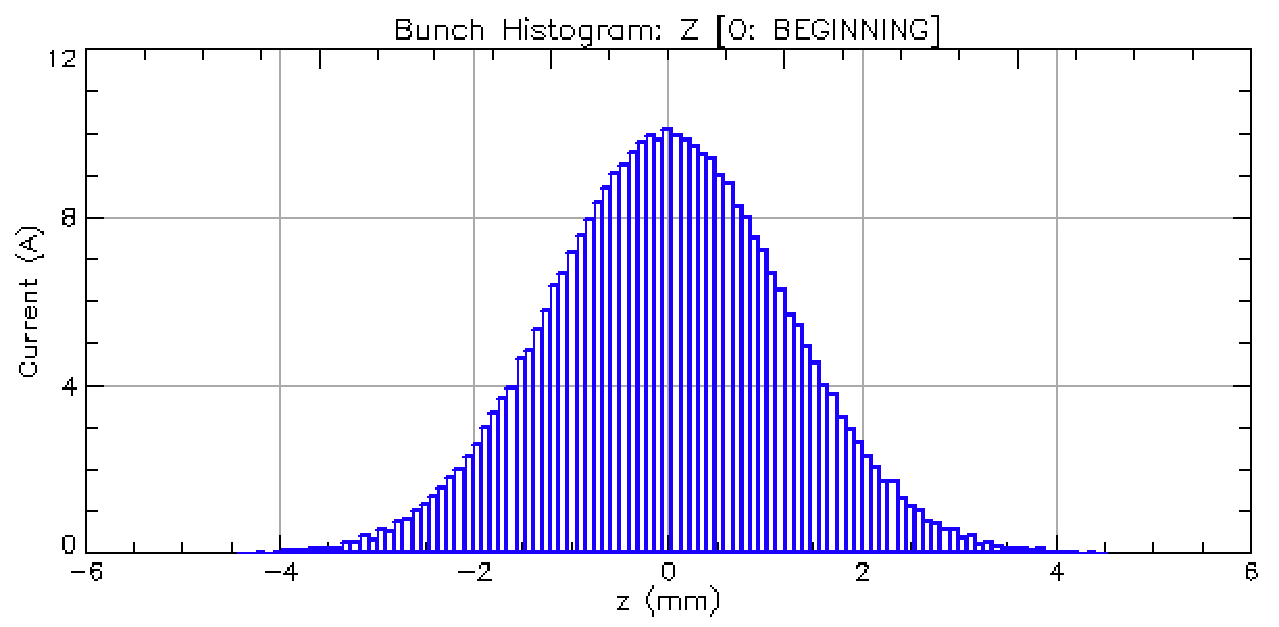
\includegraphics[width=5in]{histogram.pdf}
  \caption{Example histogram plot.}
  \label{f:histogram}
\end{figure}

For a \vn{"histogram"} type graph, \vn{curve%data_type} determines what coordinate is plotted along
the x-axis.  Valid \vn{curve%data_type} values are:
\index{x}\index{px}\index{y}\index{py}\index{z}\index{pz}
\begin{example}
  "x"
  "px"
  "y"
  "py"
  "z"
  "pz"
  "intensity"       -- Photon total intensity 
  "intensity_x"     -- Photon intensity along x-axis 
  "intensity_y"     -- Photon intensity along y-axis
  "phase_x"         -- Photon phase along x-axis
  "phase_y"         -- Photon phase along y-axis
\end{example}
In this example above, the $x$-axis of the plot will correspond to the $z$ phase space coordinate.

The maximum and minimum of the bins is set automatically to fit the data.  The
\vn{curve%hist%number} establishes the number of bins. Alternatively, if \vn{curve%hist%number = 0},
then \vn{curve%hist%width} establishes
 the width of the histogram bins and sets the number automatically. 

If \vn{curve%hist%density_normalized = T}, then the height of a bin will be divided by its width. If
\vn{curve%hist%weight_by_charge = T}, then the particle charge will be used to bin, otherwise the
particle count will be used to bin.

The \vn{curve%hist%center} will insure that a bin will be centered at this location.

\index{curve!ele_ref_name}
To change the place in the lattice where the data for the \vn{histogram} is evaluated, use the
\vn{set curve ele_ref_name} command.

If \vn{graph%type} is \vn{"histogram"} then \vn{curve%data_source} 
must be either:
\begin{example}
  "beam"
  "multi_turn_orbit"
\end{example} 
\vn{"beam"} indicates that the points of the histogram plot will be obtained correspond to the
positions of the particles within a tracked beam. \vn{multi_turn_orbit"} is used for rings where a
single particle is tracked multiple turns and the position of this particle is recorded each
turn. In this case, a \vn{d2_data} structure must have been set up to hold the turn--by--turn
orbit. This \vn{d2_data} structure must be called \vn{multi_turn_orbit} and must have \vn{d1_data}
data arrays for the histogram planes to be plotted. For example, if the histogram plot is \vn{x}
versus \vn{px}, then there must be \vn{d1_data} arrays named \vn{"x"} and \vn{"px"}. The number of
turns is determined by the setting of \vn{ix_max_data} in the \vn{tao_d1_data} namelist
(\sref{s:init.data}).

%%-----------------------------------------------------------------
%\subsection{Drawing the Beam Chamber Wall}
%\index{beam chamber wall}
%\label{s:beam.wall.draw}
%
%If a beam chamber wall has been defined in the lattice file, This wall can be drawn in a \vn{curve}
%by setting \vn{curve%type} to \vn{"beam_chamber_wall"}.
%
%Beam chamber walls are drawn, like a \vn{lat_layout}, on a one dimensional line as a function of
%longitudinal position along the machine centerline.
%
%Note: Use the command \vn{show ele -wall} to print information about the beam chamber wall for a
%particular element.

%%-----------------------------------------------------------------
%\subsection{Drawing Controller Element Curves}
%\index{drawing controller element curves}
%\label{s:draw.control}
%
%A controller element is a \bmad lattice element that controls the parameters of other elements.
%There are three types of controller elements: \vn{groups}, \vn{overlays}, and \vn{rampers}. See 
%the Bmad manual for more details. A controller has one or more independent variables that control
%parameters of other elements. The response of a controlled parameter as a function of any one of 
%controller variables may be plotted.

%% Put under graph%type:
%%  "control_curve"      ! Plot slave response for a controller lattice element (\sref{s:draw.control})


%-----------------------------------------------------------------
\subsection{Drawing a Key Table}
\index{key table}
\label{s:key.table}

The \vn{key table} is explained more fully in Section~\sref{s:key.bind}.  An example is shown in
Figure~\ref{f:layout.table}. A template to create a key table looks like:
\begin{example}
  &tao_template_plot
    plot%name = "table" 
    plot%n_graph = 1
  /

  &tao_template_graph
    graph%type = "key_table" 
    graph_index = 1
    graph%n_curve = 0
  /
\end{example}

The number in the upper left corner, to the left of the first column, (\vn{1} in
Fig.~\ref{f:layout.table}) shows the active \vn{key bank}. The columns in the Key Table are:
\begin{example}
  Ix         ! Key index.
  Name       ! Element name whose attribute is bound.
  Attrib     ! Name of the element attribute that is bound.
  Value      ! Current value of bound attribute.
  Value0     ! Initial value of bound attribute.
  Delta      ! Change in value when the appropriate key is pressed.
  Uni        ! Universe that contains the element.
  Opt        ! Shows if bound attribute is used in an optimization.
\end{example}

Note that in a \vn{Lattice Layout}, if a displayed element has a bound attribute, then the key index
number will be displayed just above the element's glyph.

The \vn{key_table} is drawn with respect to the upper left hand corner of the region in which it is
placed.

%-----------------------------------------------------------------
\subsection{Phase Space Plotting}
\index{phase space plotting}
\label{s:phase.space}

\begin{figure}
  \centering
  \begin{subfigure}[b]{0.45\textwidth}
    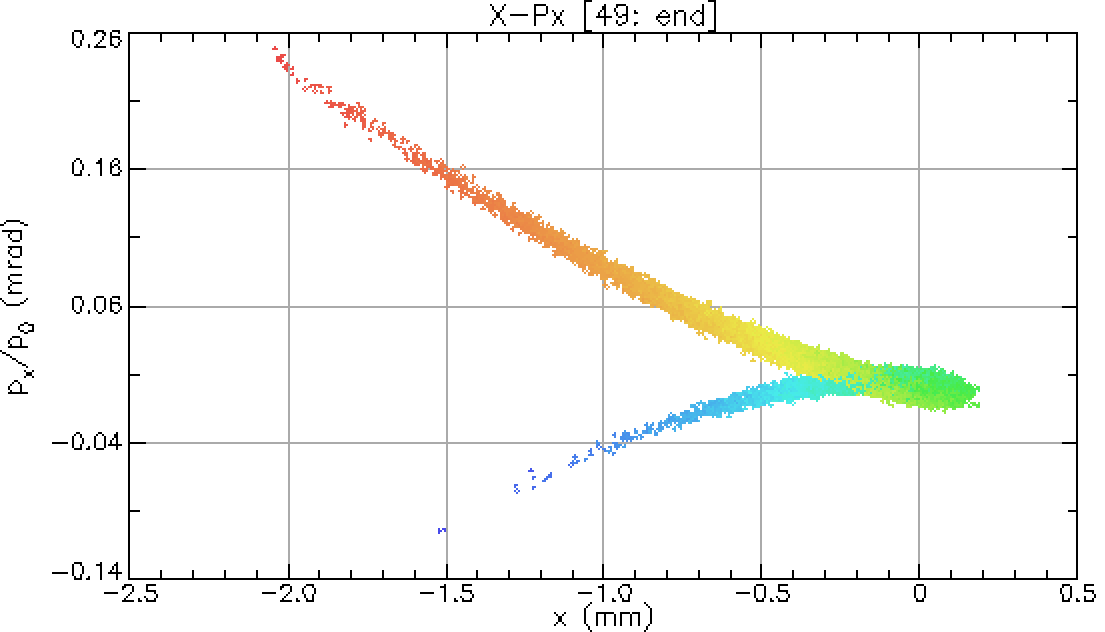
\includegraphics[width=\textwidth]{plot-color-xpx}
    \caption{Horizontal phase space}
  \end{subfigure}
  \begin{subfigure}[b]{0.45\textwidth}
    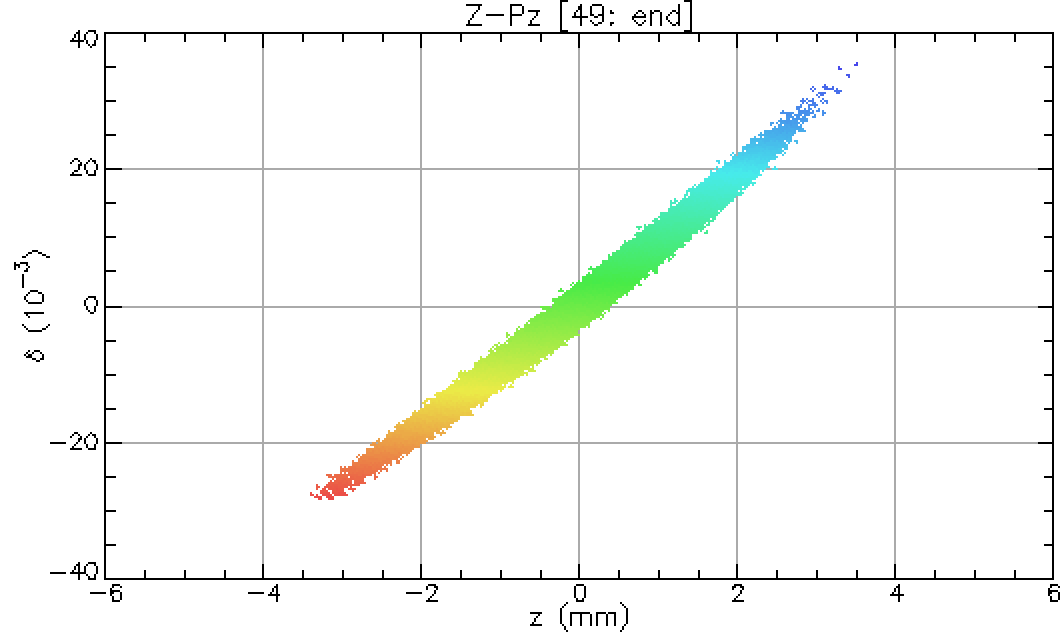
\includegraphics[width=\textwidth]{plot-color-zpz}
    \caption{Longitudinal phase space}
  \end{subfigure}  
  \caption{Example Phase Space plot, with points colored by the \vn{pz} coordinate.}
  \label{f:phase.space}
\end{figure}

A \vn{phase space} plot displays a particle or particles phase space coordinates at a given
location. Phase space plotting is associated with a \vn{graph} by setting \vn{graph%type} equal to
\vn{"phase_space"}. The concepts here are similar to data plotting (\sref{s:plot.data}). An example
is show in Figure~\ref{f:phase.space}.  Example Phase Space template:
\begin{example}
&tao_template_plot
  plot%name = "xphase"
  plot%x%min =   -2.5
  plot%x%max = 0.5
  plot%x%label = "x (mm)"
  plot%n_graph = 1
/

&tao_template_graph
  graph_index = 1
  graph%name = "x"
  graph%type = "phase_space"
  graph%box = 1, 1, 1, 1
  graph%title = "X-Px"
  graph%margin =  0.15, 0.06, 0.12, 0.12, "%BOX"
  graph%x_axis_scale_factor = 1000.00 !m->mm
  graph%y%label =  "p\textbackslash{}dx\textbackslash{}u/p\textbackslash{}d0\textbackslash{}u (mrad)"
  graph%y%major_div = 4
  graph%n_curve = 1
  graph%y%label_offset=.4
  curve(1)%data_type = "x-px" 
  curve(1)%y_axis_scale_factor = 1000 !rad->mrad
  curve(1)%data_source = "beam_tracking"
  curve(1)%ele_ref_name = "END"
  curve(1)%symbol%type = 1
  curve(1)%data_type_z = "pz"
  curve(1)%use_z_color = T
  /
\end{example}

For a \vn{"phase_space"} type graph, \vn{curve%data_type_x} determines what phase space coordinate
is plotted along the x-axis and \vn{curve%data_type} determines what phase space coordinate is
plotted along the y-axis. The phase space coordinates are:
\index{x}\index{px}\index{y}\index{py}\index{z}\index{pz}
\begin{example}
  "x"
  "px"
  "y"
  "py"
  "z"
  "pz"
  "intensity"       -- Photon total intensity 
  "intensity_x"     -- Photon intensity along x-axis 
  "intensity_y"     -- Photon intensity along y-axis
  "phase_x"         -- Photon phase along x-axis
  "phase_y"         -- Photon phase along y-axis
\end{example}
In this example above, the $x$-axis of the plot will correspond to the $z$ phase space coordinate
and the $pz$-axis will correspond to the $px$ coordinate.

\index{curve!ele_ref_name}
To change the place in the lattice where the data for the \vn{phase_space} curve is evaluated, use
the \vn{set curve ele_ref_name} command.

Points can be colored by another phase space coordinate by activating \vn{use_z_color = T}.  The
available curve options and defaults are:
\begin{example}
  use_z_color = F
  data_type_z = "" 
  z_color0 = 0
  z_color1 = 0
  autoscale_z_color = T
\end{example}
These can be the init file, or in Tao using the \vn{set curve} command.  The \vn{data_type_z} can be
set to any of the available phase space coordinates.  \vn{z_color0} and \vn{z_color1} specify the
minimum and maximum of this coordinate to be used in the color range. Values above or below this
range will be colored Black or Grey, respectively.  If \vn{autoscale_z_color=T}, then these will be
set automatically based on the limits of the \vn{data_type_z} coordinate.

If \vn{graph%type} is \vn{"phase_space"} then \vn{curve%data_source} 
must be either:
\begin{example}
  "beam"
  "multi_turn_orbit"
  "twiss"
\end{example} 
\vn{"beam"} indicates that the points of the phase space plot will be obtained correspond to the
positions of the particles within a tracked beam. \vn{multi_turn_orbit"} is used for rings where a
single particle is tracked multiple turns and the position of this particle is recorded each
turn. In this case, a \vn{d2_data} structure must have been set up to hold the turn--by--turn
orbit. This \vn{d2_data} structure must be called \vn{multi_turn_orbit} and must have \vn{d1_data}
data arrays for the phase space planes to be plotted. For example, if the phase space plot is \vn{x}
versus \vn{px}, then there must be \vn{d1_data} arrays named \vn{"x"} and \vn{"px"}. The number of
turns is determined by the setting of \vn{ix_max_data} in the \vn{tao_d1_data} namelist
(\sref{s:init.data}). Using \vn{"twiss"} as the \vn{curve%data_source} indicates that the phase
space plot will be an ellipse whose shape is based upon the Twiss and coupling parameters, and the
normal mode emittances. If the normal mode emittances have not been computed then a nominal value of
1e-6~m-rad is used.

%-----------------------------------------------------------------
\subsection{Parametric Plotting}
\label{s:param.plot}

With parametric plotting, both the $x$ and the $y$ values of the points on a curve are dependent
upon an independent parameter. An example could be plotting $\alpha_a(s)$ versus $\sqrt{\beta_b(s)}$ over
some range of the independent parameter $s$. One way to do parametric plotting is to use data slices
as discussed in section~\sref{s:graph.data.slice}. Another way to do parametric plotting, which is
discussed in this section, is to setup two plot curves whose $y$ values are the desired dependent
parameters ($\alpha_x(s)$ and $\beta_y(s)$ say) and then define a parametric curve which uses the
data from these curves.

The two curves from which the data is to be taken must be in the same graph. The $y$ values from the
first curve will be taken to define the $x$ coordinate of the parametric curve and the $y$ values
from the second curve will be taken to define the $y$ coordinate of the parametric curve. The plot
that holds these curves will be called the ``\vn{source}'' plot. Example:
\begin{example}
  &tao_template_plot
   plot%name = "src"
   plot%x_axis_type = "s"
   plot%n_graph = 1
  /

  &tao_template_graph
   graph_index = 1
   graph%name = "g"
   graph%n_curve = 2
   curve(1)%data_source = "lat"
   curve(1)%data_type = "alpha.a"
   curve(2)%data_source = "lat"
   curve(2)%data_type = "expression: sqrt(beta.b)"
\end{example}
This defines a source plot called \vn{src} with two curves which will be used in the parametric plot. 

The parametric plot curve references the source curves by setting the parametric curve's
\vn{data_source} parameter equal to \vn{"curve"} and the parametric curve's \vn{data_type} to the
graph in the source plot which contains the source curves. For example:
\begin{example}
  &tao_template_plot
    plot%name = "parametric"
    plot%n_graph = 1
    plot%x_axis_type = "curve"
  /

  &tao_template_graph
    graph_index = 1
    graph%name = "g1"
    graph%n_curve = 1
    curve(1)%data_source = "curve"
    curve(1)%data_type = "src.g"
  /
\end{example}
The parametric plot's \vn{x_axis_type} needs to be set to \vn{"curve"} along with the parametric
curve's \vn{data_source}.

When the parametric plot is \vn{placed} in the plot window, \tao will look for a suitable source
plot to connect with. If \tao does not find a suitable source plot, \tao will place a source plot in
an unused plot \vn{region} and set the plot to be invisible. The region name will be set to
\begin{example}
  <source-plot-name>_<parametric-plot-region>
\end{example}
where \vn{<source-plot-name>} is the name of the source plot and \vn{<parametric-plot-region>} is
the name of the region where the parametric plot has been placed. For example, if the above
parametric plot is placed in a region called ``\vn{r12}'', the name of the region where the source
plot is placed will be named ``\vn{src_r12}''. Note: The \vn{show plot} command will show if a plot
in a given region is visible. The \vn{set plot} (\sref{s:set.plot}) command can be used to toggle 
plot visibility.

%-----------------------------------------------------------------
\subsection{QuickPlot Plotting}
\label{s:line.symb}

\vn{QuickPlot} is an interface library developed for \bmad for graphics plotting. QuickPlot uses
the following concepts:
\begin{example}
  PAGE  -- The entire drawing surface.
  BOX   -- The area that the graph with axes, titles, etc. is placed into.
  GRAPH -- The actual plotting area within the bounds of the axes.
\end{example}

For text that has an associated \vn{justify} parameter, the \vn{justify} parameter is a two
character string.  The first character gives the horizontal justification:
\begin{example}
   "L" -- Left justify
   "C" -- Center justify
   "R" -- Right justify
\end{example}
The second character gives the vertical justification
\begin{example}
   "B" -- Bottom justify
   "C" -- Center justify
   "T" -- Top justify
\end{example}

For text that has an associated \vn{units} parameter, the \vn{units} parameter is a character string
which is divided up into three parts. The syntax of the \vn{units} parameter is:
\begin{example}
   "unit_type/ref_object/corner"
\end{example}
Where \vn{unit_type} is the type of units:
\begin{example}
   "%"       - Percent.
   "DATA"    - Data units.
   "MM"      - millimeters.
   "INCH"    - Inches.
   "POINTS"  - Printers points (72 points = 1 inch, 1 pt ~ 1 pixel).
\end{example}
\vn{ref_object} is a reference object (optional except if \vn{unit_type} = "\%").
\begin{example}
   "PAGE"  -- Relative to the page.
   "BOX"   -- Relative to the box.
   "GRAPH" -- Relative to the graph.
\end{example}
And \vn{corner} is the origin location (optional):
\begin{example}
   "LB" -- Left Bottom.
   "LT" -- Left Top.
   "RB" -- Right Bottom.
   "RT" -- Right Top.
\end{example}

\vn{QuickPlot} defines a number of structures to parameterize such things like line and symbol
properties. The structures that \tao uses are as follows.

The \vn{qp_axis_struct} structure defines the properties of a graph axis
\begin{example}
  type qp_axis_struct
    label             = "<string>" ! Axis label string.
    min               = <real>     ! Min is the left or bottom axis number.
    max               = <real>     ! Max is the right or top axis number.
    number_offset     = <real>     ! Offset from axis line in inches.
    label_offset      = <real>     ! Offset from numbers in inches.
    major_tick_len    = <real>     ! Major tick length in inches.
    minor_tick_len    = <real>     ! Minor tick length in inches.
    label_color       = <string>   ! Color of the label string
    major_div         = <integer>  ! Number of major divisions
    major_div_nominal = <integer>  ! Major divisions nominal value.
    minor_div         = <integer>  ! Minor divisions. 0 = Tao will choose.
    minor_div_max     = <integer>  ! Max minor div number if Tao chooses.
    places            = <integer>  ! Number of digits to print
    type              = <string>   ! Axis type: "LINEAR" or "LOG".
    bounds            = <string>   ! Axis bounds: "GENERAL", "ZERO_AT_END", etc.
    tick_side         = <integer>  ! 1 = draw to the inside, 0 = both, -1 = outside.
    number_side       = <integer>  ! 1 = draw to the inside, -1 = outside.
    draw_label        = <logical>  ! Draw the label string
    draw_numbers      = <logical>  ! Draw the numbers.
  end type
\end{example}

The \vn{%bounds} parameter sets how the axes min and max values are calculated.
Possible settings are:
\begin{example}
  "ZERO_AT_END"      ! Min or max value is set to zero.
  "ZERO_SYMMETRIC"   ! Min and max chosen so that max = -min.
  "GENERAL"          ! No restrictions.
  "EXACT"            ! The User min/max is used.
\end{example}
Example \tao session:
\begin{example}
Tao> set graph r13 y%bounds = "zero_at_end"
Tao> scale r13 200 280   ! Graph bounds set to [0, 300]

Tao> set graph r13 y%bounds = "zero_symmetric"
Tao> scale r13 200 280   ! Graph bounds set to [-300, 300]

Tao> set graph r13 y%bounds = "general"
Tao> scale r13 20 190    ! Graph bounds set to [0, 200]

Tao> set graph r13 y%bounds = "exact"
Tao> scale r13 20 190    ! Graph bounds set to [20, 190]
\end{example}

\begin{table}
\begin{tabular}{ll} \toprule
{\B}u       & Start a superscript or end a subscript \\[0.3ex]
{\B}d       & Start a subscript or end a superscript.
              {\B}u and {\B}d must always be used in pairs \\[0.3ex]
{\B}b       & Backspace (i.e., do not advance text pointer  
               after plotting the previous character) \\[0.3ex]
{\B}fn      & Switch to Normal font (1)       \\[0.3ex]
{\B}fr      & Switch to Roman font (2)        \\[0.3ex]
{\B}fi      & Switch to Italic font (3)       \\[0.3ex]
{\B}fs      & Switch to Script font (4)       \\[0.3ex]
{\B}{\B}    & Backslash character (\B)        \\[0.3ex]
{\B}x       & Multiplication sign ($\times$)  \\[0.3ex]
{\B}.       & Centered dot ($\cdot$)          \\[0.3ex]
{\B}A       & Angstrom symbol (\AA)         \\[0.3ex]
{\B}gx      & Greek letter corresponding to roman letter x. See Table~\ref{t:greek}. \\[0.3ex]
{\B}mN {\B}mNN & Graph marker number \vn{N} or \vn{NN} (1-31) \\[1ex]
{\B}(NNNN)  & 
\parbox{5.2in} {Character number NNNN (1 to 4 decimal digits) from the Hershey character set which
includes a number of special characters including mathematical, musical, astronomical, and
cartographical symbols.} \\ \bottomrule
\end{tabular}
\caption{Escape Sequences for Labels.}
\label{t:plot.escape}
\end{table}

The \vn{major_div} parameter is not settable directly. Rather, \vn{major_div_nominal} may be set by
the user and then \tao will calculate the value of \vn{major_div} such that the value of
\vn{major_div} is ``close'' to the value of \vn{major_div_nominal} with the constraint that the value
of \vn{major_div} ``nicely'' divides the range from given by the values for \vn{min} and \vn{max}.

The \vn{places} parameter set the number of places to display a number. \tao will automatically
calculate this number and it is not user settable.

The \vn{label} parameter may include Greek letters, subscripts, superscripts, and special characters.
Encoding for these are given in Table~\ref{t:plot.escape}. 

The \vn{label_color} parameter sets the color of the label string. Possible settings for the color are:
\begin{example}
  White   (actually the background color)       Orange          
  Black   (actually the foreground color)       Yellow_Green    
  Red                                           Light_Green         
  Green                                         Navy_Blue       
  Blue                                          Purple          
  Cyan                                          Reddish_Purple  
  Magenta                                       Dark_Grey        
  Yellow                                        Light_Grey       
\end{example}
Color names are case insensitive.

Table~\ref{t:greek} shows how the character string \vn{"{\B}g<r>"}, where \vn{"<r>"} 
is a Roman letter, map onto the Greek character set.
\begin{table}
  \centering
  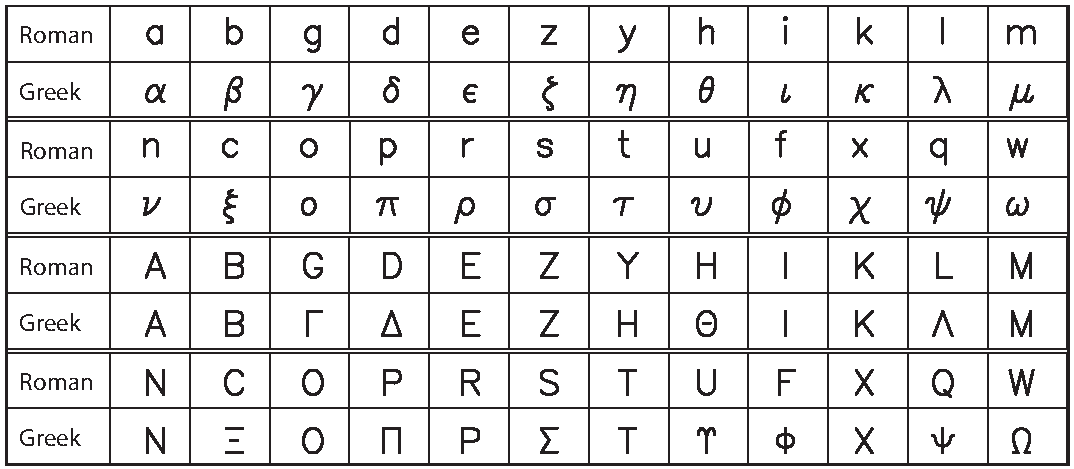
\includegraphics[width=5.0in]{greek.pdf}
  \caption[Roman to Greek Character Conversion]{Conversion for the string 
\vn{"{\B}g<r>"} where \vn{"<r>"} is a Roman character to the corresponding 
Greek character.}
\label{t:greek}
\end{table}

The parameters associated with data lines drawn in a graph are contained in the \vn{qp_line_struct}:
\begin{example}
  type qp_line_struct
    width          = <integer>  ! Default = 1
    color          = <string>   ! Default = "black"
    pattern        = <string>   ! Default = "solid"
  end type
\end{example}

The possible colors for a line are given above. The \vn{pattern} parameter sets how the line is
drawn. Possible settings are:
\begin{example}
  solid      ! Solid line                 dotted     ! Dotted line             
  dashed     ! Dashed line                dash_dot3  ! Dash--dot--dot--dot line
  dash_dot   ! Dash--dot line
\end{example}
Pattern names are case insensitive.

The parameters associated with symbols that are drawn are contained in the \vn{qp_symbol_struct}:
\begin{example}
  type qp_symbol_struct
    type          = <string>  ! Default = "dot"
    height        = <real>    ! Size in points. Default = 10
    color         = <string>  ! Default = "black"
    fill_pattern  = <string>  ! Default = "solid_fill"
    line_width    = <integer> ! Default = 1.
  end type
\end{example}

Possible \vn{fill_pattern} settings are:
\begin{example}
  solid_fill                    hatched           
  no_fill                       cross_hatched     
\end{example}
Fill pattern names are case insensitive.

The symbol types are:
\begin{example}
  square                 triangle                    square_concave              
  dot                    circle_plus                 diamond                     
  plus                   circle_dot                  star5                       
  times                  square_filled               triangle_filled           
  circle                 circle_filled               red_cross                 
  x                      star5_filled                star_of_david             
\end{example}
These symbols are illustrated in Table~\ref{t:plot.syms}. Symbol type names are case insensitive.

\begin{table}
  \centering
  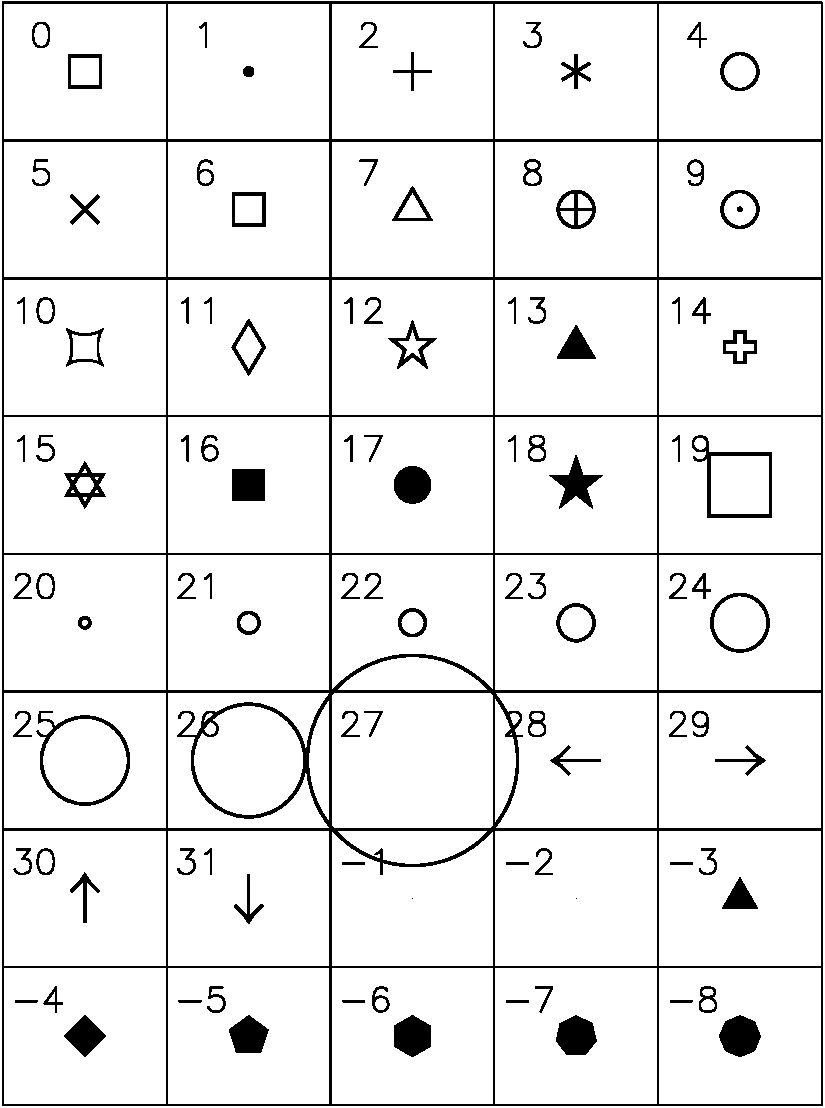
\includegraphics[width=5in]{plot-syms.pdf}
  \caption{Plotting Symbols.}
  \label{t:plot.syms}
\end{table}

\chapter{Tao Line Mode Commands}
\label{c:command}

This chapter gives a description of the commands that \tao knows about
in \vn{line mode}. Commands are case sensitive. The list of commands
is shown in Table~\ref{t:commands}.\index{Commands!Command List}

%%  ---------------------------------------------------------------------
Multiple commands may be entered
on one line using the ``;'' character as a separator.


\begin{table}[h]
\centering {\tt
\begin{tabular}{|l|l||l|l|} \hline
  {\it Command} & {\it Section}  & {\it Command} & {\it Section} \\ \hline
  alias      & \ref{s:alias}    &  restore      & \ref{s:restore} \\ \hline
  call       & \ref{s:call}     &  reinitialize & \ref{s:reinit}  \\ \hline
  change     & \ref{s:change}   &  run          & \ref{s:run}     \\ \hline
  clip       & \ref{s:clip}     &  scale        & \ref{s:scale}   \\ \hline
  derivative & \ref{s:deriv}    &  set          & \ref{s:set}     \\ \hline
  exit       & \ref{s:exit}     &  show         & \ref{s:show}    \\ \hline 
  flatten    & \ref{s:flatten}  &  single-mode  & \ref{s:sing}    \\ \hline
  help       & \ref{s:help}     &  spawn        & \ref{s:spawn}   \\ \hline
  history    & \ref{s:history}  &  use          & \ref{s:use}     \\ \hline
  output     & \ref{s:output}   &  veto         & \ref{s:veto}    \\ \hline
  place      & \ref{s:place}    &  view         & \ref{s:view}    \\ \hline
  plot       & \ref{s:plot}     &  x-axis       & \ref{s:x-axis}  \\ \hline
  quit       & \ref{s:quit}     &  x-scale      & \ref{s:x-scale} \\ \hline
\end{tabular}}
\caption{Table of \tao commands.}
\label{t:commands}
\end{table}

%%Don't display anything after this by default!!! ---------------------

\index{Arithmetic expressions} 
The \tao command prompt parser can handle arithmetic expressions. 
Arithmetic expressions can be used in a place where a real value is required.
The standard operators are defined: \hfil\break
\hspace*{0.15in}
\begin{tabular}{ll}
  $a + b$           & Addition        \\
  $a - b$           & Subtraction     \\
  $a \, \ast \, b$  & Multiplication  \\
  $a \; / \; b$     & Division        \\
  $a \, \land \, b$ & Exponentiation  \\
\end{tabular} \newline
The following intrinsic functions are also recognized: \hfil\break
\index{Intrinsic functions}
\hspace*{0.15in}
\begin{tabular}{ll}
  \vn{sqrt}(x)      & Square Root    \\
  \vn{log}(x)       & Logarithm      \\
  \vn{exp}(x)       & Exponential    \\
  \vn{sin}(x)       & Sine           \\
  \vn{cos}(x)       & Cosine         \\
  \vn{tan}(x)       & Tangent        \\
  \vn{asin}(x)      & Arc sine       \\
  \vn{acos}(x)      & Arc cosine     \\
  \vn{atan}(x)      & Arc Tangent    \\
  \vn{abs}(x)       & Absolute Value \\
  \vn{ran}()        & Random number between 0 and 1 \\
  \vn{ran_gauss}()  & Gaussian distributed random number with unit RMS \\
\end{tabular} \newline
Both \vn{ran} and \vn{ran_gauss} use a seeded random number generator. 
Setting the seed is described in Section~\ref{s:globals}.

For a description of \vn{single mode} commands see
Chapter~\ref{c:single}. To put \tao into \vn{single mode} use the
\vn{single_mode} command. 

\vfil
\break

%% alias --------------------------------------------------------------
\section{Alias}\index{Commands!alias}
\label{s:alias}

Format: 
\begin{example}
  alias \{<alias_name> <string>\}
\end{example}

\vskip 0.2in

\vn{Alias} is like Unix aliases and allows the defining of alias
commands. Using the \vn{alias} command without any arguments results
in a printout of the aliases that have been defined. When using an
alias up to 9 arguments may be substituted in the \vn{<string>}. The
i\Th argument is substituted in place of the sub-string ``[[i]]''.
arguments that do not have a corresponding ``[[i]]'' are placed at the end
of \vn{<string>}

Examples:
\begin{example}
    alias xyzzy plot [[1]] model  ! Define xyzzy
    alias                         ! Show all aliases
    xyzzy top                     ! Use an alias
    plot top model                ! Equivalent to "xyzzy top"
    xyzzy top abc                 ! Equivalent to "plot top model abc"
\end{example}
In the above example ``xyzzy'' is the alias for the string ``plot [[1]]
model''.  When the command xyzzy is used ``top'' is substituted
for ``[[1]]'' in the string.

%% call --------------------------------------------------------------
\section{Call}\index{Commands!call}
\label{s:call}

Format: 
\begin{example}
  call <filename> \{<arg_list>\}  \Strut
\end{example}

\vskip 0.2in 
\vn{call} opens a command file and executes the commands
in it.  \tao first looks in the current directory for the file. If not
found \tao will look in the directory pointed to by the
\vn{TAO_COMMAND_DIR} directory.  Up to 9 arguments may be passed to
the command file. The i\Th argument is substituted in place of the
string ``[i]'' in the file. Nesting of command files (command files
calling other command files) is allowed. There is no limit to the
number of nestings, however, only one argument list is allowed. This
argument list is specified by the call to the first command file. Any
nested command files can use this argument list.

Do loops are allowed with the following syntax:
\begin{example}
  do <var> <begin> <end> <step> 
    ...
    tao command [<var>]
    ...
  enddo
\end{example}
\vn{<var>} can be any character string up to 10 characters long.
The \vn{<var>} can be used as a variable in the loop body but must be
bracketed.  The step size can be any integer positive or negative but not zero.
Nested loops are allowed. Command files can be called within do loops.

Examples:
\begin{example}
    call my_cmd_file abc def 
\end{example}
In the above example the argument ``abc'' is substituted for any
``[[1]]'' appearing the file and ``def'' is substituted for any
``[[2]]''.
\Newline

\begin{example}
  do i 1 100
    call set_quad_misalignemnt [[i]] ! command file to misalign quadrupoles
    zero_quad 1e-5*2^([[i]]-1) ! Some user supplied command to zero quad number [[i]]
  enddo
\end{example}

%% change --------------------------------------------------------------
\section{Change}\index{Commands!change}
\label{s:change}

Format:
\begin{example}
  change ele <name_or_number> <attribute> <number>
  change var <name> <locations> <number>
  change bunch_start <coordinate> <number>
\end{example}

\vskip 0.2in \vn{change} changes element attribute values or variable
values in the \vn{model} lattice. To set, say, datum values, etc. use
the \vn{set} command.

Generally \vn{<number>} is added to the existing value of the
attribute or variable. That is:
\begin{example}
  final_value = initial_value + <number>
\end{example}
If "@" is prepended to \vn{<number>} then just the value of
\vn{<number>} is used to set the value
\begin{example}
  final_value = <number>
\end{example}
If "d" is prepended to \vn{<number>} then the value relative to the design
value is used:
\begin{example}
  final_value = design_value + <number>
\end{example}

For linear lattices, \vn{change bunch_start <coordinate> <number>} 
can be use to vary the starting coordinates where \vn{<coordinate>} is one of: 
\begin{example}
  (x, p_x, y, p_y, z, p_z)
\end{example}
For circular lattices only the \vn{p_z} component is applicable. 
Also for linear lattices, \vn{change ele beginning <twiss>} can be used to
vary the starting Twiss parameters where \vn{<twiss>} is one of:  
\begin{example}
  beta_x, beta_y, alpha_x, alpha_y 
  eta_x, eta_y,etap_x, etap_y    
\end{example}

Examples:
\begin{example}
  change ele 124 x_offset  0.1     ! Offset element #124 by 0.1
  change ele q02w k1 d 1.2e-2      ! set the k1 strength of q02w relative to the design
  change var steering[34:36] @1e-3 ! set the steering strength #34-36 to 0.001
  change var steering[*] @0.0      ! set all steering strengths to 0.0
  change bunch_start x @0.001      ! set beginning x position to 1 mm
\end{example}


%% clip --------------------------------------------------------------
\section{Clip}\index{Commands!clip}
\label{s:clip}

Format:
\begin{example}
  clip \{<where> <limit1> <limit2>\}
\end{example}

\vskip 0.2in \vn{clip} vetoes data points for optimizing. If points are vetoed
and either measured or reference data is being plotted then the points clipped
will no longer be plotted. The points vetoed are those points whose $y$ values
are outside a certain range defined by \vn{<limit1>} \vn{<limit2>}. If neither
\vn{<limit1>} nor \vn{<limit2>} is present then the clip range is taken to be
outside the graph minimum and maximum $y$--axis values. If only \vn{<limit1>} is
present then the clip range is outside the range from -\vn{<limit1>} to
+\vn{<limit1>}. If both are present than the range is from \vn{<limit1>} to
\vn{<limit2>}.  The graphs that are clipped is determined by the \vn{<where>}
switch.  If \vn{<where>} is not present all graphs are scaled.

Examples
\begin{example}
  clip top.x -3  7  ! clip the x graph in the top region
  clip bottom       ! clip the graphs in the bottom region
\end{example}

%% exit --------------------------------------------------------------
\section{Exit}\index{Commands!exit}
\label{s:exit}

Format:
\begin{example}
  exit
\end{example}

\vskip 0.2in
\vn{Exit} exits the program. Same as \vn{Quit}.

%% derivative --------------------------------------------------------------
\section{Derivative}\index{Commands!derivative}
\label{s:deriv}

Format:
\begin{example}
  derivative
\end{example}

\vskip 0.2in \vn{Derivative} calculates the \vn{dModel/dVariable}
matrix needed for the \vn{lm} optimizer.

%% flatten --------------------------------------------------------------
\section{Flatten}\index{Commands!flatten}
\label{s:flatten}

Format:
\begin{example}
  flatten <optimizer>
\end{example}

\vskip 0.2in
\vn{Flatten} runs the optimizer to minimize the merit function. This is the 
same as \vn{run}. See the \vn{run} command for more details.

%% help --------------------------------------------------------------
\section{Help}\index{Commands!help}
\label{s:help}

Format:
\begin{example}
  help <command>
\end{example}

\vskip 0.2in 
\vn{Help} gives help on \tao commands. The environmental
variable \vn{TAO_DIR} must be defined so \tao can find any help files.

Examples:
\begin{example}
  help run   ! Gives help on the run command
\end{example}

%% history --------------------------------------------------------------
\section{History}\index{Commands!history}
\label{s:history}

Format:
\begin{example}
  history           ! Print the command history.
  history <number>  ! Reinvoke a command by number.
  history <string>  ! Reinvoke last command that begins with <string>.
\end{example}

\vskip 0.2in
Every \tao command entered is recorded in a ``history stack'' and
these commands can be viewed and reinvoked as needed. 

Examples
\begin{example}
  history 34   ! Reinvoke command number 34.
  history set  ! Reinvoke last set command.  
\end{example}

%% output --------------------------------------------------------------
\section{Output}\index{Commands!ouput}
\label{s:output}

Format:
\begin{example}
  output curve <curve_name> \{<file_name>\} ! Write the curve data
  output digested \{<file_name>\}  ! Write a digested Bmad lattice file of the model.
  output gif \{<file_name>\}       ! create a gif file of the plot window.
  output hard                    ! print the plot window to a printer.
  output lattice \{<file_name>\}   ! Write a Bmad lattice file of the model
  output ps \{<file_name>\}        ! create a postscript file of the plot window.
  output var \{<file_name>\}       ! Write a Bmad file of variable values.
\end{example}

\vskip 0.2in The \vn{output} command creates various files. If \vn{<file_name>} is
not given then the defaults are:
\begin{example}
  curve.dat                       ! output curve
  digested8_lat_universe_#.bmad   ! output digested
  quick_plot.gif                  ! output gif
  lat_universe_#.bmad             ! output lattice
  quick_plot.ps                   ! output ps
  global%var_out_file             ! optput var
\end{example}
where \vn{\#} is replaced by the universe number. 

Note: PGPLOT does a poor job producing gif files so consider
making a postscript file instead and using the pstogif unix command to
convert.

%% place --------------------------------------------------------------
\section{Place}\index{Commands!place}
\label{s:place}

Format:
\begin{example}
  place <region> <template>
  place <region> none
\end{example}

\vskip 0.2in 
The \vn{place} command is used to associate a \vn{<template>} plot
with a \vn{<region>} and thus create a visible plot in that region. To
erase a plot from a region use the \vn{none} switch. Notice that by
using multiple \vn{place} commands a \vn{template} can be associated
with more than one region.

Examples:
\begin{example}
  place top orbit  ! place the orbit template in the top region
  place top none   ! erase any plots in the top region
\end{example}

%% plot --------------------------------------------------------------
\section{Plot}\index{Commands!plot}
\label{s:plot}

Format:
\begin{example}
  plot <region> <who>
\end{example}

\vskip 0.2in 
The \vn{plot} command is used to determine who is plotted
in the graphs of a given region. Use a ``-'' for baselines. 

Examples:
\begin{example}
  plot bottom model - design       ! Plot model - design in the bottom region
  plot top meas - model + design - ref 
\end{example}

%% quit --------------------------------------------------------------
\section{Quit}\index{Commands!quit}
\label{s:quit}

Format:
\begin{example}
  quit
\end{example}

\vskip 0.2in
\vn{Quit} exits the program. Same as \vn{exit}.

%% restore --------------------------------------------------------------
\section{Restore}\index{Commands!restore}
\label{s:restore}

Format:
\begin{example}
  restore data  <data_name> <locations>
  restore var <var_name> <locations>
\end{example}

\vskip 0.2in 
The \vn{restore} command cancels data or variable
vetoes. See also the \vn{use}
and \vn{veto} commands.

Examples:
\begin{example}
  restore data orbit.x[23,34:56]   ! unveto orbit.x data.
  restore data orbit.x[23,34:56:2] ! unveto orbit.x 23 and even datums between 34 and 56
  restore data *@orbit[34]         ! unveto orbit data in all universes.
  restore var quad_k1[67]          ! unveto variable
\end{example}

%% reinitialize -------------------------------------------------------
\section{Reinitialize}\index{Commands!reinitialize}
\label{s:reinit}

Format:
\begin{example}
  reinitialize \{<init_file>\}
\end{example}

\vskip 0.2in Reinitializes \tao. This can be useful to reset everything to
initial conditions or to perform analysis with more than one initialization file.
If \vn{<init_file>} is not given then 
the current initialization file is used. If \vn{init_file} = \vn{default} then
the default initialization file \vn{tao.init} is used.

Examples:
\begin{example}
  reinitialize 
  reinit tao_special.init !reinitializes \tao with the initialization file 
                           \vn{tao_special.init}
\end{example}


%% run --------------------------------------------------------------
\section{Run}\index{Commands!run}
\label{s:run}

Format:
\begin{example}
  run \{<optimizer>\}
\end{example}

\index{de!optimizer}\index{lm!optimizer}
\vskip 0.2in The \vn{run} command runs an optimizer. If
\vn{<optimizer>} is not given then the default optimizer is used. To
stop the optimizer before it is finished press the period ``.''
key. If you want the optimizer to run forever run the optimizer in
\vn{single mode}. Valid optimizers are:
\begin{example}
  lm            ! Levenburg-Marquardt
  de            ! Differential Evolution
\end{example}

Examples:
\begin{example}
  run 
  run de
\end{example}

%% scale --------------------------------------------------------------
\section{Scale}\index{Commands!scale}
\label{s:scale}

Format:
\begin{example}
  scale \{<where> <value1> <value2>\}
\end{example}

\vskip 0.2in 
\vn{scale} adjusts the vertical scale of graphs. If neither
\vn{<value1>} nor \vn{<value2>} is present then the scale is adjusted
so that all the data points are within the graph region.  If only
\vn{<value1>} is present then the scale is taken to be from
-\vn{<value1>} to +\vn{<value1>}. If both are present than the scale
is from \vn{<value1>} to \vn{<value2>}.  The graphs that are scaled is
determined by the \vn{<where>} switch. If \vn{<where>} is not present
or \vn{<where>} is ``all'' then all graphs are scaled.

Examples:
\begin{example}
  scale top.x -3  7  ! scale the x graph in the top region
  scale bottom       ! scale the graphs in the bottom region
  scale              ! scale everything
\end{example}


%% set --------------------------------------------------------------
\section{Set}\index{Commands!set}
\label{s:set}

Format:
\begin{example}
  set curve <curve> <component> = <value>
  set data <data_name>|<component> = <value>
  set global <component> = <value>
  set graph <graph> <component> = <value>
  set lattice <component> = <value>
  set plot_page <component> = <value1> \{<value2>\}
  set universe <universe> <on/off> <recalculate>
  set var <var_name>|<component> = <value>
\end{example}

\vskip 0.2in 
The \vn{set} command is used to set values for datums,
variables, etc.  For setting element attributes in the \vn{model}
lattice use the \vn{change} command.

To apply a set to all data or variable classes use ``*''
in place of \vn{<data_name>} or \vn{var_name}.

For \vn{set curve}, the \vn{<component>}s that can be set are:
\begin{example}
  ele_ref_name   ! Name of reference element
  ix_ele_ref     ! Index of reference element
\end{example}

For \vn{set data}, the \vn{<component>}s that can be set are:
\begin{example}
  base        ! Base model value
  design      ! Design model value
  meas        ! Measured data value.
  ref         ! Reference data value.
  weight      ! Weight for the merit function.
  exists      ! Valid datum for computations?
  good_meas   ! A valid measurement has been taken?
  good_ref    ! A valid reference measurement has been taken?
  good_opt    ! Good for using in the merit function for optimization?
  good_plot   ! Good for using in a plot?
  good_user   ! This is what is set by the use, veto, and restore commands.
\end{example}
Besides a numeric value \vn{<value>} can be any of the above along with:
\begin{example}
  meas        ! Measured data value.
\end{example}
\vskip 0.2in

For \vn{set graph}, the \vn{component}s that can be set are:
\begin{example}
  who(<n>)    = <string>
  who(<n>)    = <string>, <integer>
  clip        = <logical>
  ix_universe = <number>
\end{example}
\vskip 0.2in

For \vn{set global}, the \vn{<component>}s that can be set are:
\begin{example}
  y_axis_plot_dmin  = <number> ! Minimum y_max-y_min allowed for a graph.
  n_opti_cycles     = <number> ! Number of optimization cycles
  lun_command_file  = <number> ! unit number for a command file.
                               !  0 -> no command file.
  bunch_to_plot     = <number> ! View data for this bunch
  prompt_string     = <string> ! Prompt String
  optimizer         = <string> ! optimizer to use. 'de', 'lm' etc...
  var_limits_on     = T/F      ! Respect the variable limits?
  plot_on           = T/F      ! Update plot window?
  opt_with_ref      = T/F      ! use reference data in optimization?
  opt_with_base     = T/F      ! use base data in optimization?
  label_lattice_elements = T/F ! For lat_layout plots
  label_keys        = T/F      ! For lat_layout plots
  derivative_recalc = T/F      ! Recalc before each optimizer run?
  lattice_recalc    = T/F      ! recalculate the lattice?
  print_command     = <string> ! Command used to print plot page
  default_init_file = <string> ! When reinitializing use this init file
  var_out_file      = <string> ! variable output data in this file
  opt_var_out_file  = <string> ! optimizer output data in this file
\end{example}
\vskip 0.2in

For \vn{set lattice}, the \vn{<component>}s that can be set are:
\begin{example}
  model      ! Model lattice value.
  base       ! Base lattice value
\end{example}
\vn{<value>} can be:
\begin{example}
  model       ! model lattice value.
  base        ! base lattice value.
  design      ! design lattice value
\end{example}
\vskip 0.2in

For \vn{set plot_page}, the \vn{<component>}s that can be set are:
\begin{example}
  title        = <string>          ! Set the plot title text
  subtitle     = <string>          ! Set the subtitle text
  subtitle_loc = <number> <number> ! Set the subtitle location (\%PAGE)
\end{example}
The \vn{subtitle_loc} component can be used to place the subtitle anywhere on
the plot page. This can be useful for referencing a noteworthy part of a graph
data.
\vskip 0.2in

For \vn{set var}, the \vn{<component>}s that can be set are:
\begin{example}
  model       ! Model lattice value.
  base        ! Base model value
  design      ! Design model value
  meas        ! Value at the time of a measurement.
  ref         ! Value at the time of a reference measurement.
  weight      ! Weight for the merit function.
  exists      ! Does this variable actually correspond to something?
  good_var    ! The optimizer can be allowed to vary it
  good_opt    ! Good for using in the merit function for optimization?
  good_plot   ! Good for using in a plot?
  good_user   ! This is what is set by the use, veto, and restore commands.
  step       ! Sets what a "small" variation of the variable is.
\end{example}
\vskip 0.2in

\vn{set universe} will turn the specified universe on or off. Turning
a universe off is useful to speed up lattice calculations when this
universe is not being used. Or, if many changes are to be performed to
a universe and there is no need to do any lattice calculations between
commands then turning off all universes will speed things up. To turn off 
the currently viewed universe use the command \vn{set universe 0 off}. 
To turn off all universes use the command \vn{set universe * off}. 
This flag only affects the lattice calculation. 
Issueing \vn{change, use, veto,} etc...  commands to a turned off uinverse
will still affect the
universe, however any lattice calculations will not be performed until
the universe is turned back on.  To recalculate the turned on lattices
when issueing a \vn{set universe} command then use \vn{set universe
<universe> <on/off> recalc}. Otherwise, no lattice calculation will
be performed until an appropriate command is called afterwards.  If
optimizing while one or more universes are turned off then the
variables associated with that universe will still be included in the
merit function but not the data for that universe. The variables will
still vary in the turned off universe.

Examples:
\begin{example}
  set data *|ref = *|meas                   ! Set all ref data = measured data in current universe.
  set data 2@orbit.x|base = 2@orbit.x|model ! Set the ref orbit.x data in universe 2 to meas
  set graph orbit.x who(1) = model          ! Plot the model orbit in the graph
  set graph orbit.x who(2) = design, -1     ! With the previous line: Plot model - design 
  set var quad\_k1 weight = 0.1             ! Set quad\_k1 weights. 
  set lattice *&|model = *&|design          ! Resets model lattice to the design in all universes
\end{example}

%% show --------------------------------------------------------------
\section{Show}\index{Commands!show}
\label{s:show}

Format:
\begin{example}
  show alias                     
  show constraints
  show data \{<data_name>\} 
  show ele <ele_name>
  show global
  show hom
  show lattice <locations>
  show optimizer
  show opt_vars
  show plot \{<template_plot_name>\}
  show plot \{<plot_region_name>\}
  show plot <graph_name>
  show plot <curve_name>
  show top10
  show var \{<var_name> <locations>\}
  show var <universe_number>@
  show write ...
\end{example}

\vskip 0.2in \vn{Show} is used to display various information about
the state of \tao.  \vn{Show write} writes to a file as well as
printing the information at the terminal. The file name is set by
\vn{global%write_file} which has the default value of
\vn{tao_show.dat}. Results are appended to the output file whan
\vn{show write} is used multiple times. If separate files are desired
then if \vn{global%write_file} has a \vn{*} character in it, a three
digit number is substituted for the \vn{*}. The value of the number
starts at \vn{001} and increases by 1 each time \vn{show write} is
used.

\begin{description}
  \item[show alias]
Shows a list of defined aliases. See the \vn{alias} command for more
details.

  \item[show constraints]
Lists data and variable constraints.

  \item[show data]
Shows data information. If \vn{<data_name>} and \vn{<locations>} are not
present shown is a list of d2\_data names.

  \item[show ele]
This shows information on lattice elements. \vn{<ele_name>} can
contain wild--card characters ``\%'' and ``*''. ``\%'' matches to any
single character and ``*'' matches to any number of characters. If
\vn{<ele_name>} contains a wild card then a list of elements that
match the name are shown. If no wild--card is present then information
about the element whose name matches \vn{<ele_name>} is shown. All
data types associated with the element will also be
listed. \vn{<ele_name>} is a number $n$ then the $n$\Th element in the
lattice list will be shown.

  \item[show global]
Shows global information.

  \item[show hom]
Shows long--rang higher order mode information for linac accelerating cavities.

  \item[show lattice]
Shows Twiss and orbit data for the \vn{model} lattice at the specified
regular element locations. If \vn{<locations>} is \vn{all} then the
entire lattice will be shown. If \vn{<locations>} is not present then
the length of the lattice will be shown.

  \item[show optimizer]
Shows information pertinent to optimization: Data and variables used, etc.

  \item[show opt\_vars]
Shows the settings of the variables used in the optimization using the 
Bmad standard lattice input format.

  \item[show plot]
Shows which templates are being plotted and in which regions and also all
available templates. See \sref{s:plot_overview} for the syntax on plot, graph, and
curve names.

  \item[show top10]
Shows top contributors to the merit function, dMerit/dVariable
derivatives, and Largest changes in variable value.

  \item[show var]
Shows variable information. If \vn{<var_name>} \vn{<locations>} is not
present shown is a list of v1\_var classes. If \vn{<var_name>} is
\vn{*} then the variables will be printed in Bmad lattice format.
To show variables associated with the \vn{n}th universe use
the format: \vn{show var n@}.

\end{description}

Examples:
\begin{example}
  show curve r2.g1.c3         ! Show the attributes of a curve named "c3" which is 
                              !   in the graph "g1" which is plotted in region "r2".
  show data                   ! lists d2_data arrays.
  show write data             ! Same as previous except results are also written
                              !   to a file.
  show data orbit             ! Show orbit data.
  show data orbit.x           ! list all orbit.x data elements
  show data orbit.x[35]       ! show details for orbit.x element 35
  show data orbit.x[35,86:95] ! list orbit.x elements 35 and 86 through 95
  show data orbit.x[1:100:5]  ! list every fifth orbit.x element between 1 and 100  
  show ele q*                 ! list all elements with names beginning with "q".
  show ele q10w               ! show a particular lattice element
  show ele 105                ! show element #105 in the lattice
  show lattice 50:100         ! show lattice elements 50 to 100
  show var *                  ! list variables in Bmad lattice format.
  show var 2@                 ! List all variables that control attributes in universe 2.
\end{example}

%% single-mode --------------------------------------------------------------
\section{Single-mode}\index{Commands!single-mode}
\label{s:sing}

Format:
\begin{example}
  single-mode
\end{example}

\vskip 0.2in 
This command puts \tao into \vn{single mode}. 

%% spawn --------------------------------------------------------------
\section{Spawn}\index{Commands!spawn}
\label{s:spawn}

Format:
\begin{example}
  spawn <shell_command>
\end{example}

\vskip 0.2in
Use the \vn{spawn} command to pass a command to the command shell.  The users
default shell is used. \vn{spawn} only works in Linux and Unix environments.

Examples:
\begin{example}
  spawn gv quick_plot.ps &      ! view a postcript file with ghostview
                                ! (and return to the TAO prompt)
  spawn tcsh                    ! launch a new tcsh shell 
                                ! (type 'exit' to return to TAO)
\end{example}

%% use --------------------------------------------------------------
\section{Use}\index{Commands!use}
\label{s:use}

Format:
\begin{example}
  use data  <data_name>
  use var <var_name>
\end{example}

\vskip 0.2in 
The \vn{use} command unvetoes data or variables and sets a veto for
the rest of the data. See also the \vn{restore} and \vn{veto}
commands.

Examples:
\begin{example}
  use data orbit.x             ! use orbit.x data in the viewed universe.
  use data *@orbit[34]         ! use element 34 orbit data in all universes.
  use var quad_k1[67]          ! use variable.
  use var quad_k1[30:60:10]    ! use variables 30, 40, 50 and 60.
  use data *                   ! use all data in the viewed universe.
  use data *@*                 ! use all data in all universes.
\end{example}


%% veto --------------------------------------------------------------
\section{Veto}\index{Commands!veto}
\label{s:veto}

Format:
\begin{example}
  veto data <data_name> <locations>
  veto var <var_name> <locations>
\end{example}

\vskip 0.2in 
The \vn{veto} command vetoes data or variables. See also the
\vn{restore} and \vn{use} commands.

Examples:
\begin{example}
  veto data orbit.x[23,34:56]  ! veto orbit.x data.
  veto data *@orbit.*[34]      ! veto orbit data in all universes.
  veto var quad_k1[67]         ! veto variable
  veto var quad_k1[30:60:10]   ! veto variables 30, 40, 50 and 60
  veto data *                  ! veto all data
  veto data *[10:20]           ! veto all data from index 10 to 20 (see note)
\end{example}

Note: The command `\cmd{veto data *.*[10:20]}' will veto all d1\_data elements
within the range 10:20 \textit{using the index convention for each d1\_data
structure separately}. This may produce curious results if the
indexes for the d1\_data structures do not all point to the same lattice
elements. 

%% view --------------------------------------------------------------
\section{View}\index{Commands!view}
\label{s:view}

Format:
\begin{example}
  view <number>
\end{example}

\vskip 0.2in 
The \vn{view} command changes which universe data is taken from from
plotting.  This also sets the default universe that commands are
applied to in the absence of a star prefix.

Examples:
\begin{example}
  view 2   ! Make universe #2 the default.
\end{example}

%% x-axis --------------------------------------------------------------
\section{X-Axis}\index{Commands!x-axis}
\label{s:x-axis}

Format:
\begin{example}
  x-axis <where> <axis_type> ! Sets horizontal data type
\end{example}

\vskip 0.2in 
\vn{X-Axis} sets the \vn{plot%x_axis_type}. This determines 
what data is used for the horizontal axis. Possibilities
for \vn{<axis_type>} are:
\begin{example}
  index     -- Use data index
  ele_index -- Use data element index
  s         -- Use longitudinal position.
\end{example}
Note that \vn{index} only makes sense for data that has an index
associated with it. Also, if a data point has more that one element associated
with it \vn{ele_index} will plot the first element index (\vn{ix_ele} not
\vn{ix_ele0}).

Examples:
\begin{example}
  x-axis all s
  x-axis top index
\end{example}

%% x-scale --------------------------------------------------------------
\section{X-Scale}\index{Commands!x-scale}
\label{s:x-scale}

Format:
\begin{example}
  x-scale \{<where>\} \{<bound1>\} \{<bound2>\}  ! sets horizontal axis bounds.
\end{example}

\vskip 0.2in 
\vn{x-scale} sets the lower and upper bounds for the horizontal axis.
If both \vn{<bound1>} and \vn{<bound2>} are present then \vn{<bound1>}
is taken to be the lower (left) bound and \vn{<bound2>} is the upper
(right) bound. If only \vn{<bound1>} is present then the bounds will
be from -\vn{<bound1>} to \vn{<bound1>}. If neither is present then
autoscale will be invoked to give the largest bounds comensurate with
the data.

Example:
\begin{example}
  x-scale            ! Autoscale all x-axes.
  x-scale all 0 100  ! scale all x-axes to go from 0 to 100.
\end{example}

%% xy-scale --------------------------------------------------------------
\section{XY-Scale}\index{Commands!xy-scale}
\label{s:xy-scale}

Format:
\begin{example}
  xy-scale \{<where>\} \{<bound1>\} \{<bound2>\}  ! sets horizontal and vertical axis bounds.
\end{example}

\vskip 0.2in \vn{xy-scale} sets the lower and upper bounds for both
the horizontal vertical axes.  This is just a shortcut for doing an
\vn{x-scale} followed by a \vn{y-scale}.  If both \vn{<bound1>} and
\vn{<bound2>} are present then \vn{<bound1>} is taken to be the lower
(left) bound and \vn{<bound2>} is the upper (right) bound. If only
\vn{<bound1>} is present then the bounds will be from -\vn{<bound1>}
to \vn{<bound1>}. If neither is present then autoscale will be invoked
to give the largest bounds comensurate with the data.

Example:
\begin{example}
  xy-scale            ! Autoscale all axes.
  xy-scale all -1 1  ! scale all axes to go from -1 to 1.
\end{example}


\chapter{Single Mode}\index{Single mode}
\label{c:single}

\tao has two \vn{modes} for entering commands. In \vn{Single Mode},
described in this chapter, each keystroke represents a command.  That
is, the user does not have to press the carriage control key to signal
the end of a command (there are a few exceptions which are noted
below). Conversely, in \vn{Line Mode}, which is described in
Chapter~\sref{c:command}, \tao waits until the \vn{return} key is
depressed to execute a command. That is, in Line Mode a command
consists of a single line of input.  Single Mode is useful for quickly
varying parameters to see how they affect a lattice but the number of
commands in Single Mode is limited.

From \vn{line mode} use the \vn{single-mode} command (\sref{s:sing})
to get into \vn{single mode}. To go back to \vn{line mode} type
"\vn{Z}".

%% key_table ------------------------------------------------------------------------
\section{Key Bindings}\index{Key Bindings}
\label{s:key_bind}

The main purpose of Single Mode is to associate certain keys with
certain variables so that the pressing of these keys will change their
associated variable. This is called a \vn{key binding}.  Key bindings
are established via the \vn{key_bindings} initialization namelist (See
Section~\sref{s:init_key_bind}). The variables are divided into banks of
10. The 0\Th bank uses variables \vn{key(1)} through \vn{key(10)} from
the \vn{key_bindings} namelist, the 1\St bank uses variables
\vn{key(11)} through \vn{key(20)}, etc.  

At any one time, only one bank is active. To see the status of this
bank, a \vn{key table} plot can be setup as shown in
Figure~\ref{f:key_table}. The relationship between the keys and a
change in a variable is:
\begin{example}
                 Change by factor of:          
     Variable    -10  -1    1     10
   ----------    ---  ---  ---  -------
    1 + 10*ib     Q    q    1   shift-1   ("!")
    2 + 10*ib     W    w    2   shift-2   ("@")
    3 + 10*ib     E    e    3   shift-3   ("\#")
    4 + 10*ib     R    r    4   shift-4   ("\$")
    5 + 10*ib     T    t    5   shift-5   ("%")
    6 + 10*ib     Y    y    6   shift-6   ("^")
    7 + 10*ib     U    u    7   shift-7   ("\&")
    8 + 10*ib     I    i    8   shift-8   ("*")
    9 + 10*ib     O    o    9   shift-9   ("(")
   10 + 10*ib     P    p    0   shift-0   (")")
\end{example}
In the above table ib is the bank number (0 for the 0\Th bank, etc.),
and the change is in multiples of the \vn{step} for a variable as
specified in the \vn{key_bindings} namelist. 

Initially the 0Th bank is active. The left arrow and right arrow are
used to decrease or increase the bank number.  Additionally the
"\vn{<}" and "$>$" keys can be used to change the deltas for the
variables.

For example, looking at Figure~\ref{f:key_table}, the \vn{"1:"} in
the upper left corner of the \vn{Key Table} shows that the 1\St bank
is active which corresponds to keys \vn{key(11)} through \vn{key(20)}
from the \vn{key_bindings} namelist.  Since, in this case, keys
\vn{key(19)} and \vn{key(20)} have not been defined, the corresponding
rows in the \vn{Key Table} are blank.

\vn{key(14)} is associated with the \vn{"4"} key and from the \vn{Key
Table} it is seen that the bound attribute is the \vn{b1_gradient} of
the element named \vn{Q15_2}.  Thus, if the \vn{"4"} key is depressed
in single mode, the value of the \vn{b1_gradient} of element
\vn{Q15_2} will be increased by the given Delta (0.1000 in this
case). Pressing the \vn{"r"} key (which is just below the \vn{"4"}
key) will decrease the value of the \vn{b1_gradient} by 0.1000. Using
the shift key, which is shift-4 (\vn{"\$"}) will increase
\vn{b1_gradient} by 10 times the given delta (1.000 in this case) and
\vn{"R"} will decrease by 10 time the given delta.

Since element \vn{Q15_2} is also displayed in the \vn{Lattice Layout},
there is a \vn{"4"} drawn above this element that reflects the fact
that the element contains a bound attribute. Since, in this case, the
Lattice Layout only shows part of the lattice, not all key indexes are
present.

%------------------------------------------------------------------------

\begin{figure}
  \centering
  \includegraphics[width=5in]{layout_graph_table.eps}
  \caption[Example key table with a lattice layout and data plots.]
{A lattice layout plot (top) above a data plot (middle) 
which in turn is above a key table plot (bottom). The points on the
curves in the data plot mark the edges of the elements displayed in
the lattice layout. Elements that have attributes that are varied as
shown in the key table have the corresponding key table number printed
above the element's glyph in the lattice layout.}
  \label{f:key_table}
\end{figure}

%% keys ------------------------------------------------------------------------
\section{List of Key Strokes}\index{Single Mode!List of Key Strokes}
\label{s:keys}

In the following list, certain commands use multiple key strokes. For
example, the \vn{"/v"} command is invoked by first pressing the slash
(\vn{"/"}) key followed by the \vn{"v"} key. \vn{"a $<$left\_arrow$>$"}
represents pressing the \vn{"a"} key followed by the left-arrow key.

\begin{description}
\item[?]
Type a short help message.

\item[a $<$left\_arrow$>$]
Pan plots left by half the plot width.

\item[a $<$right\_arrow$>$]
Pan plots right by half the plot width.

\item[a $<$up\_arrow$>$]
Pan plots up by half the plot height.

\item[a $<$down\_arrow$>$]
Pan plots down by half the plot height.

\item[s $<$left\_arrow$>$]
Scale x-axis of plots by a factor of 2.0.

\item[s $<$right\_arrow$>$]
Scale x-axis of plots by a factor of 0.5

\item[s $<$up\_arrow$>$]
Scale y-axis of plots by a factor of 2.0.

\item[s $<$down\_arrow$>$]
Scale y-axis of plots by a factor of 0.5


\item[z $<$left\_arrow$>$]
Zoom x-axis of plots by a factor of 2.0.

\item[z $<$right\_arrow$>$]
Zoom x-axis of plots by a factor of 0.5

\item[z $<$up\_arrow$>$]
Zoom y-axis of plots by a factor of 2.0.

\item[z $<$down\_arrow$>$]
Zoom y-axis of plots by a factor of 0.5

\item[c]  
Show constraints.

\item[g]
Go run the default optimizer. The optimizer will run until you type a
'.' (a period).  Periodically during the optimization the variable
values will be written to files, one for each universe, whose name is
\vn{tao_opt_vars\#.dat}. where \vn{\#} is the universe number.

\item[v]
Show variable values in bmad compatible lattice format. See also the
\vn{/v} and \vn{\W v} commands.

\item[V] 
Same an \vn{v} except only only variables used in the optimization are printed.

\item[Z] 
Go back to \vn{line mode}

\item[$<$]
Reduce the deltas (the amount that a variable is changed when you use
the keys 0 through 9) of all the variables by a factor of 2.

\item[$>$]
Increase the deltas (the amount that a variable is changed when you
use the keys 0 through 9) of all the variables by a factor of 2.

\item[$<$left\_arrow$>$]
Shift the active key bank down by 1: ib -$>$ ib - 1

\item[$<$right\_arrow$>$]
Shift the active key bank up by 1: ib -$>$ ib + 1

\item[/$<$up\_arrow$>$]
Increase all key deltas by a factor of 10.

\item[/$<$down\_arrow$>$]
Decrease all key deltas by a factor of 10.

\item[$<$CR$>$]
Do nothing but replot.

\item[-p]
Toggle plotting. Whether to plot or not to plot is initially
determined by plot%enable.

\item['$<$command$>$]
Accept a Line Mode (\sref{c:command}) command.

\item[/e $<$Index or Name$>$]
Prints info on a lattice element. If there are two lattices being used
and only the information of an element from one particular lattice is
wanted then prepent with "n@" where n is the lattice
index.

\item[/l]
Print a list of the lattice elements with Twiss parameters.

\item[/s $<$min$>$ $<$max$>$]
Set the scale min and max values for all the plots. This is the same
as setting p%y%min and p%y%max in the \tao input file. If \vn{min} and
\vn{max} are not given then an autoscale will be done.

\item[/u $<$Universe Index$>$]
Switch the viewed universe.

\item[/v]
Write variable values to the default output file.  The default output
file name is set by \vn{global%var_out}. This file is in BMAD
format. See also the \vn{V} command.

\item[/x $<$min$>$ $<$max$>$]
Set the horizontal scale (longitudinal position) min and max values
for all the plots. This is the same as setting p%x%min and p%x%max in
the \tao input file. If \vn{min} and \vn{max} are not given then the scale
will be choisen to include the entire lattice. 

\item[=v $<$digit$>$ $<$value$>$]
Set variable value. \vn{<digit>} is between 0 and 9 corresponding to a
variable of the current bank. \vn{<value>} is the value to set the
variable to.

\item[=$<$right\_arrow$>$]
Set saved ("value0") values to variable values to saved values. The
saved values (the value0 column in the display) are initially set to
the initial value on startup. There are saved values for both the
manual and automatic variables. Note that reading in a TOAD input file
will reset the saved values. If you want to save the values of the
variables in this case use "/w" to save to a file. Use the
"\vn{/$<$left\_arrow$>$}" command to go in the reverse direction.

\item[=$<$left\_arrow$>$]
Paste saved ("value0") values back to the variable values.  The saved
values (the value0 column in the display) are initially set to the
initial value on startup. Use the "\vn{/$<$right\_arrow$>$}" command to go in
the reverse direction.

\end{description}


%----------------------------------------------------------------
\part{Programmer's Guide}

\chapter{Customizing Tao}
\index{Customizing}
\label{c:custom_tao}

%----------------------------------------------------------------
\section{It's all a matter of Hooks}
\index{Customizing!Hooks}

The golden rule when extending \tao is that you are only allowed to
replace routines or redefine structures that have the name ``hook'' in
them.  If you have the source code then it's within your power to
modify any routine in \tao as much as you like. However, as time goes
by, and revisions are made to the \tao routines to extend the
usefulness of \tao and to eliminate bugs, only modifying the ``hook''
routines will ensure that custom changes will have a minimum impact on
the specialized routines that will be written by various people.

\tao is written in Fortran 95 and a knowledge of Fortran is
required. However, if you know C then Fortran can be learned in a
couple of days. Because of the interoperability between C and Fortran
once the wrapper routines are written to interface with \tao the rest
of your coding can, in principle all be done in C.

\tao relies on extensive use of pointers and logical flags. However,
all of the structures you will need to use are contained in the
\vn{tao_struct.f90} module. This module is heavily documented and
provides all the information needed to use the intrinsic \tao
structures on your customizations. It is also a very good idea to have
a copy of \vn{bmad_struct.f90} handy as this contains most of the
structures used by \bmad.

%----------------------------------------------------------------
\section{Compiling your custom Tao}
\index{Customizing!Compiling}

The \tao libraries can be compiled without compiling an
executable. Here is where this comes in handy. Since the standard \tao
subroutines have already been made into libraries, all you need to do
is compile and link your custom routines with the standard \tao
subroutines into an executable.

There are 11 ``hook'' files located in the \cmd{ROOT/tao/hook}
directory. These are the files you can customize. There are two
options here.
\begin{enumerate}
  \item Change the files directly in \cmd{ROOT/tao/hook}, adding any extra
    files you may need, then recompile from the \cmd{ROOT/tao} directory with
  \cmd{gmake -f M.tao}.  \label{cust_option_one}
  \item Copy the hook files to a separate directory say \cmd{ROOT/my_tao},
    adding any extra files you may need, then write a Makefile to 
    compile and link these
    routines to the main \tao library. \label{cust_option_two}
\end{enumerate}
Option~\ref{cust_option_two} is HIGHLY recommended because it keeps
the \tao distribution tree undisturbed and reserves the possibility to
create multiple custom \tao programs using the same vanilla \tao
library. This option is used in the following example.

%----------------------------------------------------------------
\section{An Example}
\index{Customizing!Example}

As an example let's include a new data type called
\vn{particle_emittance}. This will be the non-normalized x and y
emittance as found from the Courant-Snyder invariant. This data type
will behave just like any other data type (i.e.  \vn{orbit},
\vn{phase} etc...). First, we should copy all the hook files to a
separate directory, call it \cmd{ROOT/my_tao}. Also include the main
program file from the \cmd{ROOT/tao/program} directory.  (replace
\vn{ROOT} with whatever top directory you placed the \vn{tao}
directory.)
\begin{example}
  mkdir ROOT/my_tao
  cp ROOT/tao/hook/*.f90 ROOT/my_tao
  cp ROOT/tao/program/tao_cl.f90 ROOT/my_tao/my_tao_cl.f90
\end{example}
Next we need a Makefile. The \cmd{ROOT/tao/M.tao} 
Makefile is a great starting point.
\begin{example}
  cp ROOT/tao/M.tao ROOT/my_tao/Makefile
\end{example}
Now change the following lines in your Makefile
\begin{example}
  LIB\_SRC\_DIRS := ./code ./hook
  OBJ\_SRC\_DIRS := ./program
\end{example}
to
\begin{example}
  LIB\_SRC\_DIRS :=
  OBJ\_SRC\_DIRS := ./
\end{example}
This Makefile will tell gmake to use the tao library that has already
been created (from \cmd{../tao/code} but the actual library is located
at \cmd{../lib/libtao.a})
 and then to compile
all of the hook files, including the main program file
(\cmd{my_tao_cl.f90}) into object files (everything in \cmd{./}, the
current directory).  Routines and declarations in object files always
override similarly named code in the \tao libraries so this allows for
your local hook files to override the dummy hook files in the \tao
library. The only downside to this method is it clutters your
\cmd{my_tao} directory with object files. You can always remove these
object files with \cmd{gmake clean}.

There are two more lines to alter. change
\begin{example}
  MAIN\_FILE :=
\end{example}
to
\begin{example}
  MAIN\_FILE := ./my\_tao_cl.f90
\end{example}
and finally,
\begin{example}
  MAKEFILE := M.tao
\end{example}
to
\begin{example}
  #MAKEFILE := M.tao !using default name for Makefile
\end{example}
Notice that this line is just being commented out with a `\#'. You are
now ready to make your customizations to the hook routines.

This example will only require the modification of one file:
\vn{tao_hook_evaluate_a_datum.f90}. The formula for single particle
emittance is
\Begineq
  \epsilon = \gamma x^{2} + 2 \alpha x x' + \beta x'^{2}
  \label{e:emittance}
\Endeq
Place the following code in \vn{tao_hook_evaluate_a_datum.f90} in the
\cmd{case select} construct (also add the necessary type declarations)
\begin{verbatim}
  case ('particle_emittance.x') 

    datum_value =  ( ele%x%gamma * tao_lat%orb(ix1)%vec(1)**2 + &
		     2 * ele%x%alpha * tao_lat%orb(ix1)%vec(1) * tao_lat%orb(ix1)%vec(2) + &
		     ele%x%beta * tao_lat%orb(ix1)%vec(2)**2)
    
  case ('particle_emittance.y')

    datum_value = ( ele%y%gamma * tao_lat%orb(ix1)%vec(3)**2 + &
		     2 * ele%y%alpha * tao_lat%orb(ix1)%vec(3) * tao_lat%orb(ix1)%vec(4) + &
		     ele%y%beta * tao_lat%orb(ix1)%vec(4)**2)
\end{verbatim}
This defines what is to be calculated for each \vn{particle_emittance}
datum.  There are two transverse coordinates, so two definitions need
to be made, one for each dimension.

Now you just need to declare the data types in the \cmd{tao.init} and
\cmd{tao_plot.init} files. For the sake of this example, modify the
initialization files used for this tutorial.
\begin{example}
  cp ROOT/tao/program/*.init ROOT/my_tao
  cp ROOT/tao/program/*.lat ROOT/my_tao
\end{example}

In \cmd{ROOT/my_tao/tao.init} add the following lines to the data
declarations section
\begin{example}
  &tao_d2_data
    d2_data%name = "particle_emittance" 
    universe = 0 
    n_d1_data = 2
  /

  &tao_d1_data
    ix_d1_data = 1
    d1_data%name = "x"  
    default_weight = 1
    use_same_lat_eles_as = 'orbit.x"
  /

  &tao_d1_data
    ix_d1_data = 2
    d1_data%name = "y"  
    default_weight = 1
    use_same_lat_eles_as = 'orbit.x"
  /
\end{example}

In \cmd{ROOT/my_tao/tao_plot.init} add the following lines to the end
of the file
\begin{example}
  &tao_template_plot
    plot%name = 'particle_emittance'
    plot%x%min =   0
    plot%x%max = 100
    plot%x%major_div = 10
    plot%x%label = ' '
    plot%x_axis_type = 'index'
    plot%n_graph = 2
  /
  
  &tao_template_graph
    graph%name = 'x'
    graph_index = 1
    graph%box = 1, 2, 1, 2
    graph%title = 'Horizontal Emittance (microns)'
    graph%margin =  0.15, 0.06, 0.12, 0.12, '%BOX'
    graph%y%label = 'x'
    graph%y%max =  15
    graph%y%min =  0.0
    graph%y%major_div = 4
    graph%n_curve = 1
    curve(1)%data_source = 'data_array'
    curve(1)%data_type   = 'particle_emittance.x'
    curve(1)%y_axis_scale_factor = 1e6 !convert from meters to microns
  /

  &tao_template_graph
    graph%name = 'y'
    graph_index = 2
    graph%box = 1, 1, 1, 2
    graph%title = 'Vertical Emittance (microns)'
    graph%margin =  0.15, 0.06, 0.12, 0.12, '%BOX'
    graph%y%label = 'Y'
    graph%y%max =  15
    graph%y%min =  0.0
    graph%y%major_div = 4
    graph%n_curve = 1
    curve(1)%data_source = 'data_array'
    curve(1)%data_type = 'particle_emittance.y'
    curve(1)%units_factor = 1e6 !convert from meters to microns
  /
\end{example}
These namelists are described in detail in Chapter~\ref{c:init}.

We are now ready to compile and then run the program. The \tao library
should have already been created so all you need to do is
\begin{example}
  cd ROOT/my_tao
  gmake
  ../bin/my_tao
\end{example}
Notice that the name of the custom \tao program is \cmd{my_tao}. If you run 
`\cmd{../bin/tao}' then you will run ``vanilla'' \tao.

After your custom \tao initializes type
\begin{example}
  place bottom particle_emittance
  scale
\end{example}
Your plot should look like Figure~\ref{f:plot_emittance}.

The emittance (as calculated) is not constant. This is due to
dispersion and coupling throughout the ring. \bmad provides a routine
to find the particle emittance from the twiss parameters that includes
dispersion and coupling called \vn{orbit_amplitude_calc}.

\begin{figure}
  \centering
  \includegraphics[width=5in]{plot_emittance.eps}
  \caption{Custom data type: non-normalized emittance}
  \label{f:plot_emittance}
\end{figure}

\Section{Other Customizations}

The above example just illustrates one of the customizations you can
perform on \tao.  Part III, Programmer's Guide lays out all of the
hook files and provides pointers for various customizations.


\chapter{Bmad Programming Overview}
\label{c:programming}

%-----------------------------------------------------------------------------
\section{Manual Notation}
\label{s:component}

\bmad defines a number of structures and these structures may contain
components which are structures, etc. In order to keep the text in
this manual succinct when referring to components, the enclosing
structure name may be dropped. For example, the \vn{lat_struct}
structure looks like
\begin{example}
  type lat_struct
    character(40) name               
    type (mode_info_struct) a, b, z  
    type (lat_param_struct) param    
    type (ele_struct), pointer ::  ele(:)
    type (branch_struct), allocatable :: branch(:)  
    ... etc. ...
  end type
\end{example}
In this example, ``\vn{%a}'' could be used to refer to, the \vn{a}
component of the \vn{lat_struct}.  To make it explicit that this is a
component of a \vn{lat_struct}, ``\vn{lat_struct%a}'' is an alternate
possibility. Since the vast majority of structures have the
``_struct'' suffix, this may be shortened to ``\vn{lat%a}''. A similar
notation works for subcomponents. For example, a \vn{branch_struct}
looks like
\begin{example}
  type branch_struct
    character(40) name
    integer ix_from_ele                  ! Index of branching element
    integer, pointer :: n_ele_track      ! Number of tracking elements
    integer, pointer :: n_ele_max
    type (ele_struct), pointer :: ele(:) ! Element array
    ... etc. ...
  end type
\end{example}
The \vn{ele} component of the \vn{branch} component of the
\vn{lat_struct} can be referred to using ``\vn{lat%branch%ele}'',
``\vn{%branch%ele}'', or ``\vn{%ele}''. Potentially, the last of these
could be confused with the ``\vn{lat%ele}'' component so ``\vn{%ele}''
would only be used if the meaning is unambiguous in the context.
%-----------------------------------------------------------------------
\section {The Bmad Libraries}
\label{s:libs}
\index{Bmad!distribution}

The code that goes into a program based upon \bmad is divided up into a number of libraries. The
\bmad web site has general information on the organization of these libraries including information
on obtaining and compiling programs. The \bmad web site is at:
\hfill\break
\hspace*{0.3in}
\url{https://www.classe.cornell.edu/bmad}

The \bmad libraries are divided into two groups. One group of
libraries contains ``in-house'' developed code. The other
\vn{``package''} libraries consist of ``external'' code that \bmad
relies upon.

The in-house developed code libraries are:
\begin{description}
  \index{sim_utils library}
  \item[bmad] \Newline
The \vn{bmad} library contains the routines for relativistic charged
particle simulation including particle tracking, Twiss calculations,
symplectic integration, etc., etc.
  \item[cpp_bmad_interface]
The \vn{cpp_bmad_interface} library is for interfacing \bmad with C++.  This library
defines a set of C++ classes corresponding to the major \bmad structures. Along
with this, the library contains conversion routines to move information between 
the C++ classes and the corresponding \bmad structures.
  \item[sim_utils] \Newline
The \vn{sim_utils} library contains a set of miscellaneous helper routines. 
Included are routines for string manipulation, file manipulation,
matrix manipulation, spline fitting, Gaussian random number generation, etc. 
\end{description}
%  
The \vn{package} libraries are:
\begin{description}
  \index{PTC/FPP!library}
  \item[forest] \Newline
This is the PTC/FPP (Polymorphic Tracking Code / Fully Polymorphic
Package) library of \'Etienne Forest that handles Taylor maps to any
arbitrary order (this is also known as Truncated Power Series Algebra
(TPSA)). See Chapter~\ref{c:ptc} for more details.  FPP/PTC is a
very general package and \bmad only makes use of a small part of its
features.  For more inform
ation see the FPP/PTC
manual\cite{b:ptc}. The core Differential Algebra (DA) package used
by PTC was developed by Martin Berz\cite{b:berz}.
%
  \index{fftw!library}
  \item[fftw] \Newline
FFTW is a C subroutine library for computing the discrete Fourier
transform in one or more dimensions. FFTW has a Fortran 2003 API.
%
  \index{gsl!library}
  \index{fgsl!library}
  \item[gsl / fgsl] \Newline
The Gnu Scientific Library (GSL), written in C, provides a wide range of mathematical
routines such as random number generators, special functions and least-squares
fitting. There are over 1000 functions in total. The FGSL library provides a Fortran
interface to the GSL library.
%
  \index{hdf5!library}
  \item[hdf5] \Newline
\vn{hdf5} is a library for for storing and managing data\cite{b:hdf5}. In particular, \bmad uses
this library for storing particle position data and field grid data.
%
  \index{lapack!library}
  \index{lapack95!library}
  \item[lapack / lapack95] \Newline
\vn{lapack} is a widely used package of linear algebra routines written in Fortran77. The
\vn{lapack95} library provides a Fortran95 interface to \vn{lapack}.
%
  \index{mad_tpsa!library}
  \item[mad_tpsa] \Newline
\vn{mad_tpsa} is a subset of the MAD-NG (Next Generation MAD) code\cite{b:mad.ng}. Specifically, the
\vn{mad_tpsa} library implements TPSA (Truncated Power Series Algebra). This is similar to the
\vn{FPP} code (see above). There are several advantages to using \vn{mad_tpsa} over \vn{FPP}. For one, using
\vn{mad_tpsa} is independent of \vn{PTC} so \vn{mad_tpsa} can be used along side \vn{PTC}. Another
reason is that \vn{mad_tpsa} is more flexible and better structured.
%
  \index{numerical recipes!library}
  \item[recipes] \Newline
Numerical Recipes is a set of subroutines for doing scientific computing including Runge--Kutta
integration, FFTs, interpolation and extrapolation, etc., etc. The documentation for this library is
the books ``Numerical Recipes, in Fortran, The Art of Scientific Computing'' and ``Numerical Recipes
in Fortran90, the Art of Parallel Scientific Computing''\cite{b:nr}.  The first book explains how
the subroutines work and the second book explains what the argument lists for the Fortran90 version
of the subroutines are. You do need both books if you want to use Numerical Recipes. For \bmad, this
library has been modified to handle double precision reals which is the standard for the other
libraries (See \sref{s:precision}). Additionally, some routines have been modified so that Numerical
Recipes can be built as a shared object library. If you get a compiler complaint about a call to a
Numerical Recipes routine missing a required argument, look in the code for that routine for
documentation.
%
  \index{open_spacecharge!library}
  \item[open_spacecharge] \Newline
The \vn{open_spacecharge} library provides low energy tracking with space charge effects.
%
  \index{pgplot!library}
  \item[PGPLOT] \Newline
The \vn{pgplot} Graphics Subroutine Library is a Fortran or C-callable, device-independent graphics
package for making simple scientific graphs. Documentation including a user's manual may be obtained
from the \vn{pgplot} web site at
\begin{verbatim}
    www.astro.caltech.edu/~tjp/pgplot.
\end{verbatim} 
One disadvantage of \vn{pgplot} for the programmer is that it is not the most user friendly. To
remedy this, there is a set of Fortran90 wrapper subroutines called \vn{quick_plot}.  The
\vn{quick_plot} suite is part of the \vn{sim_utils} library and is documented in
Chapter~\ref{c:quick.plot}.
%
  \index{plplot!library}
  \item[plplot] \Newline
The \vn{plplot} library is an updated version of \vn{pgplot}. The \vn{plplot} library can be used as
a replacement for \vn{pgplot}. The \vn{quick_plot} suite, which is part of the \vn{sim_utils}
library and is documented in Chapter~\ref{c:quick.plot}, provides wrapper routines for \vn{plplot}
to make things more programmer friendly.
%
  \index{xraylib!library}
  \item[xraylib] \Newline
The xraylib library provides routines for obtaining parameters pertinent to the X-ray interaction
with matter. xraylib is developed by Tom Schoonj and is hosted on github\cite{b:xraylib}

\end{description}

%-----------------------------------------------------------------------------
\section{Using getf and listf for Viewing Routine and Structure Documentation}
\label{s:getf}
\index{getf}
\index{listf}

As can be seen from the program example in Chapter~\ref{c:program.info}
there is a lot going on behind the scenes even for this
simple program. This shows that programming with \bmad can be both easy
and hard. Easy in the sense that a lot can be done with just a few
lines. The hard part comes about since there are many details that
have to be kept in mind in order to make sure that the subroutines
are calculating what you really want them to calculate.

To help with the details, all \bmad routines have in their source
files a comment block that explains the arguments needed by the
subroutines and explains what the subroutine does. To help quickly
access these comments, there are two Python scripts that are supplied
with the \bmad distribution that are invoked with the commands
\vn{listf} (``list function'') and \vn{getf} (``get function'').

The \vn{getf} command is used to locate routines and structures, and
to type out information on them.  The form of the command is
\begin{verbatim}
    getf <name>
\end{verbatim}
This searches for any routine or structure with the name
\vn{<name>}. \vn{<name>} may contain the wild--cards ``*'' and ``.'' where
``*'' matches to any number of characters and ``.'' matches to any
single character. For example:
\begin{example}
    getf bmad_parser
    getf lat_struct
    getf twiss_at_.
\end{example}
The third line in this example will match to the routine
\vn{twiss_at_s} but not the routine \vn{twiss_at_start}. You may or
may not have to put quotation marks if you use wild card characters.
As an example, the command \vn{getf twiss_struct} produces:
\begin{example}
  /home/cesrulib/cesr_libs/devel/cvssrc/bmad/modules/twiss_mod.f90
    type twiss_struct
      real(rp) beta, alpha, gamma, phi, eta, etap
      real(rp) sigma, emit
    end type
\end{example}
The first line shows the file where the structure is located (This is
system and user dependent so don't be surprised if you get a different
directory when you use \vn{getf}). The rest of the output shows the
definition of the \vn{twiss_struct} structure.  The result of issuing
the command \vn{getf relative_tracking_charge} is:
\begin{example}
  File: ../../bmad/modules/bmad_utils_mod.f90
  !+
  ! Function relative_tracking_charge (orbit, param) result (rel_charge)
  !
  ! Routine to determine the relative charge/mass of the particle being
  ! tracked relative to the charge of the reference particle.
  !
  ! Input:
  !   orbit -- coord_struct: Particle position structure.
  !   param -- lat_param_struct: Structure holding the reference particle id.
  !
  ! Output:
  !   rel_charge -- real(rp): Relative charge/mass
  !-
  function relative_tracking_charge (orbit, param) result (rel_charge)
\end{example}
The first line again shows in what file the subroutine is located. The rest of the output explains
what the routine does and how it can be called.

The \vn{getf} command can also be used to search for global integer and real parameter constants. For example
\begin{example}
  getf c_light
\end{example}
will give the result:
\begin{example}
  File: ../sim_utils/interfaces/physical_constants.f90
      real(rp), parameter :: c_light = 2.99792458d8              ! speed of light
\end{example}
[Global constants are contants defined in a module that have global scope (defined before the
\vn{contains} statement).] For parameters whose name ends with a dollar sign ``\vn{\$}'' character
(\sref{s:prog.conventions}, the dollar sign suffix may be omitted in the search string. For example
the search
\begin{example}
  getf quadrupole
\end{example}
will give the result
\begin{example}
  File: ../../bmad/modules/bmad_struct.f90
      integer, parameter :: drift$ = 1, sbend$ = 2, quadrupole$ = 3, group$ = 4, ...
\end{example}
Since the dollar sign is a special character for the Python regexp module used by \vn{getf}, to
include a dollar sign in the search string the dollar sign must be prefixed by three back
slashes. Thus the search
\begin{example}
  getf quadrupole\B\B\B$
\end{example}
will also locate the value of \vn{quadrupole\$}.

The \vn{listf} command is like the \vn{getf} command except that only
the file name where a routine or structure is found is printed.
The \vn{listf} command is useful if you
want to just find out where a routine or structure definition lives.
For example, the \vn{listf relative*} command would produce
\begin{example}
  File: ../../bmad/code/relative_mode_flip.f90
      function relative_mode_flip (ele1, ele2) result (rel_mode)

  File: ../../bmad/modules/bmad_utils_mod.f90
      function relative_tracking_charge (orbit, param) result (rel_charge)
\end{example}

The way \vn{getf} and \vn{listf} work is that they search a list of
directories to find the \vn{bmad}, \vn{sim_utils}, and \vn{tao}
libraries. Currently the libraries in the \bmad distribution that were
not developed at Cornell are not searched. This is primarily due to
the fact that, to save time, \vn{getf} and \vn{listf} make assumptions
about how documentation is arranged in a file and the non--Cornell libraries 
do not follow this format.

%-----------------------------------------------------------------------
\section{Precision of Real Variables}
\label{s:precision}
\index{programming!precision (rp)}
\index{rp}


Historically, \bmad come in two flavors: One version where the real
numbers are single precision and a second version with double
precision reals. Which version you are working with is controlled by
the kind parameter \vn{rp}\ (Real Precision) which is defined in the
\vn{precision_def} module. On most platforms, single precision
translates to \vn{rp}\ = 4 and double precision to \vn{rp}\ = 8. The
double precision version is used by default since round-off errors can
be significant in some calculations. Long--term tracking is an example
where the single precision version is not adequate. Changing the
precision means recompiling all the libraries except \vn{PTC} and
\vn{pgplot}.  You cannot mix and match. Either you are using the
single precision version or you are using the double precision
version. Currently, \bmad is always compiled double precision and it
is a near certainty that there would have to be some fixes if there
was ever a need for compiling single precision.

To define floating point variables in Fortran with the correct precision,
 use the syntax {\tt ``real(rp)''}. For example:
\begin{example}
    real(rp) var1, var2, var3
\end{example}
When you want to define a literal constant, for example to pass an
argument to a subroutine, add the suffix \vn{_rp} to the end of the
constant. For example
\begin{example}
   var1 =  2.0_rp * var2
   call my_sub (var1, 1.0e6_rp)
\end{example}
Note that \vn{2_rp} is different from \vn{2.0_rp}. \vn{2_rp} is an
integer of kind \vn{rp}, not a real.

Independent of the setting of \vn{rp}, the parameters \vn{sp} and
\vn{dp} are defined to give single and double precision numbers
respectively.

%-----------------------------------------------------------------------------
\section{Programming Conventions}
\label{s:prog.conventions}
\index{programming!conventions}

\bmad subroutines follow the following conventions:

\begin{description}

\index{\$!character to denote a parameter}
\item[A ``\$'' suffix denotes a parameter:] 
A dollar sign ``\$'' at the end of a name denotes an 
parameter. For example, in the above program, to check
whether an element is a quadrupole one would write:
\begin{verbatim}
  if (lat%ele(i)%key == quadrupole$) ...
\end{verbatim}
Checking the source code one would find in the module \vn{bmad_struct}
\begin{verbatim}
  integer, parameter :: drift$ = 1, sbend$ = 2, quadrupole$ = 3, group$ = 4
\end{verbatim}
One should always use the parameter name instead of the integer it represents.
That is, one should never write
\begin{verbatim}
  if (lat%ele(i)%key == 3) ...  ! DO NOT DO THIS!
\end{verbatim}
For one, using the name makes the code clearer. However, more
importantly, the integer value of the parameters may at times be
shuffled for practical internal reasons. The use of the integer value
could thus lead to disastrous results. 

By convention all names ending in ``\$'' are parameters. And most ``dollar sign'' parameters are
integers but there are exceptions. For example, the parameter \vn{real_garbage\$} is a real number.
To find the value of a dollar sign parameter, the \vn{getf} or \vn{listf} (\sref{s:getf}) commands
can be used.

\index{structures}
\item[Structure names have a ``_struct'' suffix:]
For example: \vn{lat_struct}, \vn{ele_struct}, etc. Structures without a 
\vn{_struct} are usually part of \'Etienne's PTC/FPP package.

\end{description}

%-----------------------------------------------------------------------
%\section {Using Modules}
%\label{s:modules}
%\index{modules}





%----------------------------------------------------------------
\begin{thebibliography}{XXXXXXX99}

\bibitem[Abell06]{b:rf.abell}
Dan Abell, ``Numerical computation of high-order transfer maps for rf cavities'',
Phys. Rev. ST Accel. Beams, vol. 9 (5) pp. 052001, (2006).

\bibitem[AML]{b:aml}
The Accelerator Markup Language / Universal Accelerator Project web page:
\hfill\break
\hspace*{0.3in}
\url{http://www.lepp.cornell.edu/~dcs/aml/}

\bibitem[Bater64]{b:batterman}
B.~Batterman, and H.~Cole,
``Dynamical Diffraction of X Rays by Perfect Crystals'',
Rev.\ Mod.\ Phys.,{\bf 36}, 3, pp.~ 681--717, (1964).

\bibitem[Berz89]{b:berz}
M. Berz, 
``Differential Algebraic Description of Beam Dynamics to Very High Orders,''
Particle Accelerators, Vol. 24, pp. 109-124, (1989).

\bibitem[Blas94]{b:blasdell}
R.~C.~Blasdell and A.~T.~Macrander, ``Modifications to the 1989 SHADOW
 ray-tracing code for general asymmetric perfect-crystal optics,''
Nuc.\ Instr.\ \& Meth. A {\bf 347}, 320 (1994).

\bibitem[Bmad]{b:bmad.web}
The Bmad web site:
\hfill\break
\hspace*{0.3in} \url{http://www.lepp.cornell.edu/~dcs/bmad}

\bibitem[Rio98]{b:del.rio}
Manuel Sanchez del Rio, ``Ray tracing simulations for crystal optics,''
Proc. SPIE 3448, Crystal and Multilayer Optics, {\bf 230} (1998). 

\bibitem[Brown77]{b:transport.appendix} 
K. L. Brown, F. Rothacker, D. C. Carey, and Ch. Iselin, ``TRANSPORT
Appendix,'' Fermilab, unpublished, (December 1977).

\bibitem[Chao93]{b:chao} 
Alexander Chao, {\em Physics of Collective Beam
Instabilities in High Energy Accelerators}, Wiley, New York (1993). 

\bibitem[Corbett99]{b:corbett}
J. Corbett and Y. Nosochkov, ``Effect of Insertion Devices in SPEAR--3,''
Proc. 1999 Part.\ Acc.\ Conf., p.~238, (1999).

\bibitem[Duff87]{b:leduff}
  J. Le Duff, \emph{Single and Multiple Touschek Effects}.
  Proc. CAS Berlin 1987,
  CERN 89-01,
  1987.

\bibitem[Forest02]{b:ptc}
E. Forest, F. Schmidt, E. McIntosh, 
{\it Introduction to the Polymorphic Tracking Code}, 
CERN–SL–2002–044 (AP), and KEK-Report 2002-3 (2002). 
Can be obtained at:
\hfill\break
\hspace*{0.3in}
\url{http://frs.web.cern.ch/frs/report/sl-2002-044.pdf}

\bibitem[Forest06]{b:geo.int}
`Etienne Forest, `Geometric integration for particle accelerators,''
J. Phys. A: Math. Gen. {\bf 39} (2006) 5321–5377.

\bibitem[Forest88]{b:quad.fringe}
E. Forest, J. Milutinovic, 
``Leading Order Hard Edge Fringe Fields Effects Exact in ($1+\delta$) and 
Consistent with Maxwell's Equations for Rectilinear Magnets,''
Nuc. Instrum. and Methods in Phys. Research A {\bf 269}, pp 474-482, (1988).

\bibitem[Forest98]{b:forest}
E. Forest, {\em Beam Dynamics: A New Attitude and Framework},
Harwood Academic Publishers, Amsterdam (1998).


\bibitem[Grote96]{b:maduser}
H. Grote, F. C. Iselin, {\it The MAD Program User's Reference Manual},
Version 8.19, CERN/SL/90-13 (AP) (REV. 5) (1996). 
Can be obtained at:
\hfill\break
\hspace*{0.3in}
\url{http://mad.home.cern.ch/mad} 

\bibitem[Healy86]{b:healy}
L. M. Healy, {\it Lie Algebraic Methods for Treating Lattice Parameter
Errors in Particle Accelerators}. Doctoral thesis, University of
Maryland, unpublished, (1986).

\bibitem[Helm73]{b:helm}
R. H. Helm, M. J. Lee, P. L. Morton, and M. Sands, ``Evaluation of Synchrotron
Radiation Integrals,'' IEEE Trans.~Nucl.~Sci. NS-20, 900 (1973).

\bibitem[Hoff06]{b:spin}
G.~Hoffstaetter, {\it Hight-Energy Polarized Proton Beams, A Modern View}, 
Springer. Springer Tracks in Modern Physics Vol~218, (2006).

\bibitem[Iselin94]{b:madphysics}
F. C. Iselin, {\it The MAD program Physical Methods Manual}, 
unpublished, (1994).  Can be obtained at: 
\hfill\break
\hspace*{0.3in}
\url{http://mad.home.cern.ch/mad}

\bibitem[Jowett87]{b:jowett} 
J. M. Jowett, ``Introductory Statistical Mechanics
for Electron Storage Rings,'' AIP Conf. Proc. 153, Physics of Part.\ Acc.,
M. Month and M. Dienes Eds., pp.~864, (1987).

\bibitem[Kohn95]{b:kohn}
V.~G.~Kohn, 
``On the Thcory of Reflectivitlby an X-Ray Multilaler Mirror''
physica status solidi (b), {\bf 187}, 61, (1995).

\bibitem[Press92]{b:nr}
W. Press, B. Flannery, S. Teukolsky, and W. Wetterling, {\em Numerical
Recipes in Fortran, the Art of Scientific Computing}, Second Edition,
Cambridge University Press, New York, (1992). \hfill \break
W. Press, B. Flannery, S. Teukolsky, and W. Wetterling, {\em Numerical
Recipes in Fortran90, the Art of Parallel Scientific Computing}, 
Cambridge University Press, New York, (1996).

\bibitem[Piwin98]{b:piwinski}
Anton Piwinski, \emph{The Touschek Effect in Strong Focusing Storage Rings}.
DESY 98-179, 1998.

\bibitem[Rosen94]{b:rosenzweig}
J. Rosenzweig and L. Serafini, ``Transverse Particle Motion in
Radio--Frequency Linear Accelerators,'' Phys Rev E, Vol. 49, p. 1599,
(1994).

\bibitem[Ruth87]{b:ruth} R. D. Ruth, ``Single-Particle Dynamics in
Circular Accelerators,'' in AIP Conference Proceedings {\bf 153}, {\em
Physics of Particle Accelerators}, pp.~152--235, M. Month and M. Dienes editors,
American Institute of Physics, New York (1987).

\bibitem[SAD]{b:sad} 
D.~Zhou and K.~Oide, ``Maps Used in SAD'' (unpublished).
Also see:
\hfill\break
\hspace*{0.3in} \url{http://acc-physics.kek.jp/SAD/}

\bibitem[Sagan03]{b:wiggler}
D. Sagan, J. Crittenden, and D. Rubin.
``A Symplectic Model for Wigglers,'' Part.\ Acc.\ Conf. (2003).

\bibitem[Sagan99]{b:coupling}
D. Sagan and D. Rubin ``Linear Analysis of Coupled Lattices,''
Phys.\ Rev.\ ST Accel.\ Beams {\bf 2}, 074001 (1999).
\hfill\break
\hspace*{20pt} 
\url{http://link.aps.org/doi/10.1103/PhysRevSTAB.2.074001}

\bibitem[Sagan06]{b:csr}
D. Sagan, ``An Efficient Formalism for Simulating the Longitudinal Kick from Coherent 
Synchrotron Radiation,'' Proc. Europ.\ Part.\ Accel.\ Conf. p. 2829 --- 31 (2006).

\bibitem[Storn96]{b:de}
R.~Storn, and K.~V.~Price, ``Minimizing the real function of the
ICEC'96 contest by differential evolution'' IEEE conf. on Evolutionary
Computation, 842-844 (1996).

\bibitem[Stoltz02]{b:boris}
P. H. Stoltz and J. R. Cary, ``Efficiency of a Boris--like Integration
Scheme with Spatial Stepping,'' Phys.\ Rev.\ Special Topics ---
Accel. \& Beams {\bf 5}, 094001 (2002).

\bibitem[Talman87]{b:talman} R. Talman, ``Multiparticle Phenomena and
Landau Damping,'' in AIP Conf.\ Proc.  {\bf 153}, {\em Physics of
Particle Accelerators}, pp.~789--834, M. Month and M. Dienes editors,
American Institute of Physics, New York (1987).

\bibitem[Tao]{b:tao}
D. Sagan, J. Smith, {\it The Tao Manual}.
Can be obtained at: \hfill\break
\hspace*{0.3in}
\url{http://www.lepp.cornell.edu/~dcs/bmad/tao_entry_point.html}

\bibitem[Rauben91]{b:tol}
T. Raubenheimer,
``Tolerances to Limit the Vertical Emittance in Future Storage Rings'', 
Particle Accelerators, 1991, {\bf 36}, pp.75-119. 
SLAC-PUB-4937 Rev., (1991).

\bibitem[Wiede99]{b:wiedemann}
H. Wiedemann, {\em Particle Accelerator Physics}, Springer, New York, 3rd Edition (2007). 

\bibitem[Wolski06]{b:wolski.coupling}
A.~Wolski,  ``Alternative approach to general coupled linear optics,''
Phys. Rev. ST Accel. Beams 9, 024001 (2006).

\bibitem[Wyckoff65]{b:wyckoff}
R. W. G. Wyckoff, {\em Crystal Structures}, Interscience Publ. (1965).

\bibitem[Schoon11]{b:xraylib} 
T. Schoonjans et al. ``The xraylib library for X-ray-matter
interactions. Recent developments,'' Spectrochimica Acta Part B: Atomic
Spectroscopy {\bf 66}, pp. 776-784 (2011).

\index{XSIF!reference}
\bibitem[Tenen01]{b:xsif}
P. Tenenbaum, ``LIBXSIF, A Stand alone Library for Parsing the Standard 
Input Format,'' Proc.\ 2001 Part.\ Acc.\ Conf.\ p. 3093 --- 95 (2001).
Documentation at
\hfill\break
\hspace*{0.3in} \url{http://www-project.slac.stanford.edu/lc/ilc/TechNotes/LCCNotes/PDF/LCC-0060%20rev.1.pdf}

\end{thebibliography}


\printindex

\end{document}
